\documentclass{article}
\usepackage{tikz}
\usepackage{booktabs}
\begin{document}
taille des requetes : 5
\begin{center}
\begin{tabular}{c c c c c c}
\toprule 
Noeuds & Requête & Noeuds & Requête & Noeuds & Requête \\
\midrule 
1, 2, 3, 4, 5 & 0 & 1, 2, 3, 4, 6 & 0 & 1, 2, 3, 5, 6 & 0 \\
1, 2, 4, 5, 6 & 0 & 1, 3, 4, 5, 6 & 0 & 2, 3, 4, 5, 6 & 0 \\
\bottomrule 
\end{tabular}
\end{center}
\\
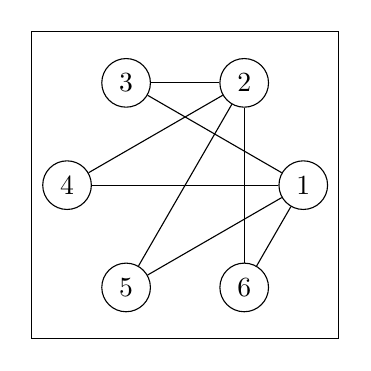
\begin{tikzpicture}
\tikzset{tinoeud/.style={draw, circle, minimum height=0.01cm}}
\clip (-2, -2) rectangle (2, 2);
\draw (-1.95, -1.95) rectangle (1.95, 1.95);
\node[tinoeud] (V1) at (0:1.5cm) {1};
\node[tinoeud] (V2) at (60:1.5cm) {2};
\node[tinoeud] (V3) at (120:1.5cm) {3};
\node[tinoeud] (V4) at (180:1.5cm) {4};
\node[tinoeud] (V5) at (240:1.5cm) {5};
\node[tinoeud] (V6) at (300:1.5cm) {6};
\draw (V1) -- (V3);
\draw (V1) -- (V4);
\draw (V1) -- (V5);
\draw (V1) -- (V6);
\draw (V2) -- (V3);
\draw (V2) -- (V4);
\draw (V2) -- (V5);
\draw (V2) -- (V6);
\end{tikzpicture}
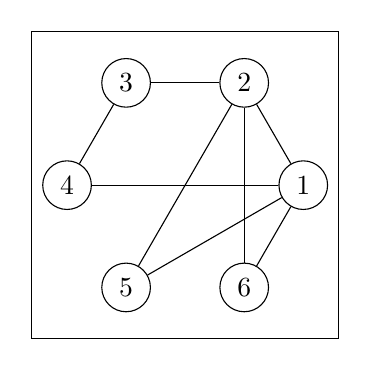
\begin{tikzpicture}
\tikzset{tinoeud/.style={draw, circle, minimum height=0.01cm}}
\clip (-2, -2) rectangle (2, 2);
\draw (-1.95, -1.95) rectangle (1.95, 1.95);
\node[tinoeud] (V1) at (0:1.5cm) {1};
\node[tinoeud] (V2) at (60:1.5cm) {2};
\node[tinoeud] (V3) at (120:1.5cm) {3};
\node[tinoeud] (V4) at (180:1.5cm) {4};
\node[tinoeud] (V5) at (240:1.5cm) {5};
\node[tinoeud] (V6) at (300:1.5cm) {6};
\draw (V1) -- (V2);
\draw (V1) -- (V4);
\draw (V1) -- (V5);
\draw (V1) -- (V6);
\draw (V2) -- (V3);
\draw (V2) -- (V5);
\draw (V2) -- (V6);
\draw (V3) -- (V4);
\end{tikzpicture}
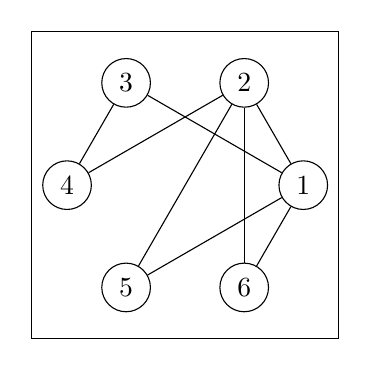
\begin{tikzpicture}
\tikzset{tinoeud/.style={draw, circle, minimum height=0.01cm}}
\clip (-2, -2) rectangle (2, 2);
\draw (-1.95, -1.95) rectangle (1.95, 1.95);
\node[tinoeud] (V1) at (0:1.5cm) {1};
\node[tinoeud] (V2) at (60:1.5cm) {2};
\node[tinoeud] (V3) at (120:1.5cm) {3};
\node[tinoeud] (V4) at (180:1.5cm) {4};
\node[tinoeud] (V5) at (240:1.5cm) {5};
\node[tinoeud] (V6) at (300:1.5cm) {6};
\draw (V1) -- (V2);
\draw (V1) -- (V3);
\draw (V1) -- (V5);
\draw (V1) -- (V6);
\draw (V2) -- (V4);
\draw (V2) -- (V5);
\draw (V2) -- (V6);
\draw (V3) -- (V4);
\end{tikzpicture}
\\
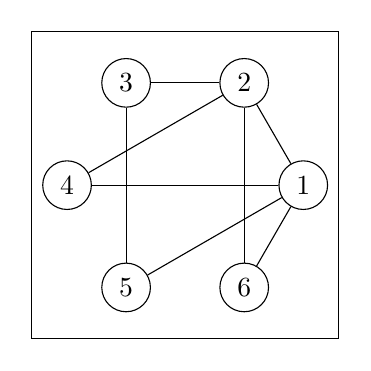
\begin{tikzpicture}
\tikzset{tinoeud/.style={draw, circle, minimum height=0.01cm}}
\clip (-2, -2) rectangle (2, 2);
\draw (-1.95, -1.95) rectangle (1.95, 1.95);
\node[tinoeud] (V1) at (0:1.5cm) {1};
\node[tinoeud] (V2) at (60:1.5cm) {2};
\node[tinoeud] (V3) at (120:1.5cm) {3};
\node[tinoeud] (V4) at (180:1.5cm) {4};
\node[tinoeud] (V5) at (240:1.5cm) {5};
\node[tinoeud] (V6) at (300:1.5cm) {6};
\draw (V1) -- (V2);
\draw (V1) -- (V4);
\draw (V1) -- (V5);
\draw (V1) -- (V6);
\draw (V2) -- (V3);
\draw (V2) -- (V4);
\draw (V2) -- (V6);
\draw (V3) -- (V5);
\end{tikzpicture}
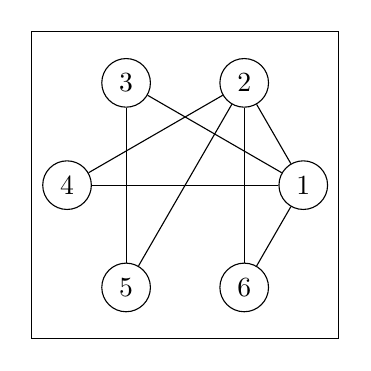
\begin{tikzpicture}
\tikzset{tinoeud/.style={draw, circle, minimum height=0.01cm}}
\clip (-2, -2) rectangle (2, 2);
\draw (-1.95, -1.95) rectangle (1.95, 1.95);
\node[tinoeud] (V1) at (0:1.5cm) {1};
\node[tinoeud] (V2) at (60:1.5cm) {2};
\node[tinoeud] (V3) at (120:1.5cm) {3};
\node[tinoeud] (V4) at (180:1.5cm) {4};
\node[tinoeud] (V5) at (240:1.5cm) {5};
\node[tinoeud] (V6) at (300:1.5cm) {6};
\draw (V1) -- (V2);
\draw (V1) -- (V3);
\draw (V1) -- (V4);
\draw (V1) -- (V6);
\draw (V2) -- (V4);
\draw (V2) -- (V5);
\draw (V2) -- (V6);
\draw (V3) -- (V5);
\end{tikzpicture}
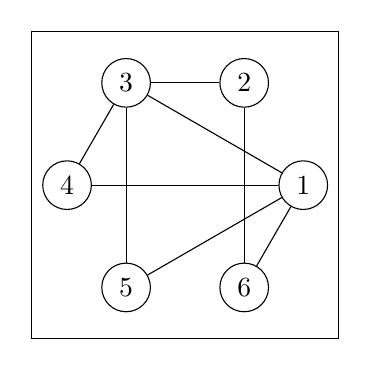
\begin{tikzpicture}
\tikzset{tinoeud/.style={draw, circle, minimum height=0.01cm}}
\clip (-2, -2) rectangle (2, 2);
\draw (-1.95, -1.95) rectangle (1.95, 1.95);
\node[tinoeud] (V1) at (0:1.5cm) {1};
\node[tinoeud] (V2) at (60:1.5cm) {2};
\node[tinoeud] (V3) at (120:1.5cm) {3};
\node[tinoeud] (V4) at (180:1.5cm) {4};
\node[tinoeud] (V5) at (240:1.5cm) {5};
\node[tinoeud] (V6) at (300:1.5cm) {6};
\draw (V1) -- (V3);
\draw (V1) -- (V4);
\draw (V1) -- (V5);
\draw (V1) -- (V6);
\draw (V2) -- (V3);
\draw (V2) -- (V6);
\draw (V3) -- (V4);
\draw (V3) -- (V5);
\end{tikzpicture}
\\
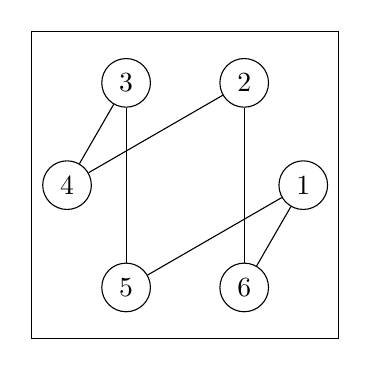
\begin{tikzpicture}
\tikzset{tinoeud/.style={draw, circle, minimum height=0.01cm}}
\clip (-2, -2) rectangle (2, 2);
\draw (-1.95, -1.95) rectangle (1.95, 1.95);
\node[tinoeud] (V1) at (0:1.5cm) {1};
\node[tinoeud] (V2) at (60:1.5cm) {2};
\node[tinoeud] (V3) at (120:1.5cm) {3};
\node[tinoeud] (V4) at (180:1.5cm) {4};
\node[tinoeud] (V5) at (240:1.5cm) {5};
\node[tinoeud] (V6) at (300:1.5cm) {6};
\draw (V1) -- (V5);
\draw (V1) -- (V6);
\draw (V2) -- (V4);
\draw (V2) -- (V6);
\draw (V3) -- (V4);
\draw (V3) -- (V5);
\end{tikzpicture}
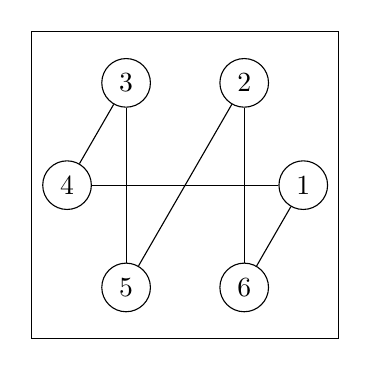
\begin{tikzpicture}
\tikzset{tinoeud/.style={draw, circle, minimum height=0.01cm}}
\clip (-2, -2) rectangle (2, 2);
\draw (-1.95, -1.95) rectangle (1.95, 1.95);
\node[tinoeud] (V1) at (0:1.5cm) {1};
\node[tinoeud] (V2) at (60:1.5cm) {2};
\node[tinoeud] (V3) at (120:1.5cm) {3};
\node[tinoeud] (V4) at (180:1.5cm) {4};
\node[tinoeud] (V5) at (240:1.5cm) {5};
\node[tinoeud] (V6) at (300:1.5cm) {6};
\draw (V1) -- (V4);
\draw (V1) -- (V6);
\draw (V2) -- (V5);
\draw (V2) -- (V6);
\draw (V3) -- (V4);
\draw (V3) -- (V5);
\end{tikzpicture}
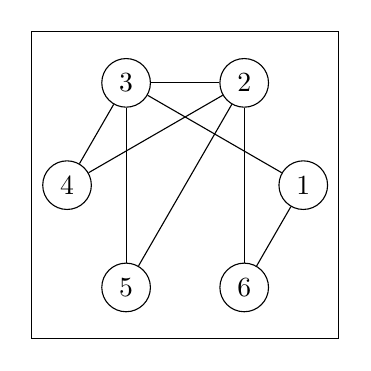
\begin{tikzpicture}
\tikzset{tinoeud/.style={draw, circle, minimum height=0.01cm}}
\clip (-2, -2) rectangle (2, 2);
\draw (-1.95, -1.95) rectangle (1.95, 1.95);
\node[tinoeud] (V1) at (0:1.5cm) {1};
\node[tinoeud] (V2) at (60:1.5cm) {2};
\node[tinoeud] (V3) at (120:1.5cm) {3};
\node[tinoeud] (V4) at (180:1.5cm) {4};
\node[tinoeud] (V5) at (240:1.5cm) {5};
\node[tinoeud] (V6) at (300:1.5cm) {6};
\draw (V1) -- (V3);
\draw (V1) -- (V6);
\draw (V2) -- (V3);
\draw (V2) -- (V4);
\draw (V2) -- (V5);
\draw (V2) -- (V6);
\draw (V3) -- (V4);
\draw (V3) -- (V5);
\end{tikzpicture}
\\
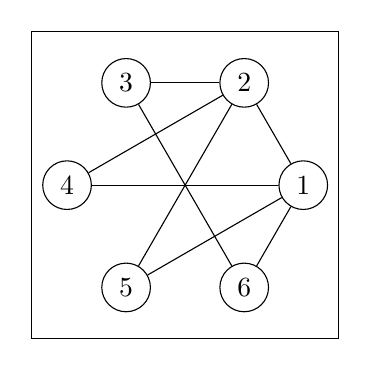
\begin{tikzpicture}
\tikzset{tinoeud/.style={draw, circle, minimum height=0.01cm}}
\clip (-2, -2) rectangle (2, 2);
\draw (-1.95, -1.95) rectangle (1.95, 1.95);
\node[tinoeud] (V1) at (0:1.5cm) {1};
\node[tinoeud] (V2) at (60:1.5cm) {2};
\node[tinoeud] (V3) at (120:1.5cm) {3};
\node[tinoeud] (V4) at (180:1.5cm) {4};
\node[tinoeud] (V5) at (240:1.5cm) {5};
\node[tinoeud] (V6) at (300:1.5cm) {6};
\draw (V1) -- (V2);
\draw (V1) -- (V4);
\draw (V1) -- (V5);
\draw (V1) -- (V6);
\draw (V2) -- (V3);
\draw (V2) -- (V4);
\draw (V2) -- (V5);
\draw (V3) -- (V6);
\end{tikzpicture}
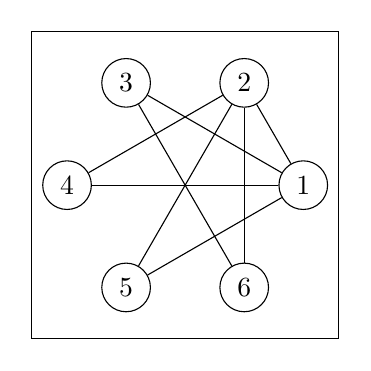
\begin{tikzpicture}
\tikzset{tinoeud/.style={draw, circle, minimum height=0.01cm}}
\clip (-2, -2) rectangle (2, 2);
\draw (-1.95, -1.95) rectangle (1.95, 1.95);
\node[tinoeud] (V1) at (0:1.5cm) {1};
\node[tinoeud] (V2) at (60:1.5cm) {2};
\node[tinoeud] (V3) at (120:1.5cm) {3};
\node[tinoeud] (V4) at (180:1.5cm) {4};
\node[tinoeud] (V5) at (240:1.5cm) {5};
\node[tinoeud] (V6) at (300:1.5cm) {6};
\draw (V1) -- (V2);
\draw (V1) -- (V3);
\draw (V1) -- (V4);
\draw (V1) -- (V5);
\draw (V2) -- (V4);
\draw (V2) -- (V5);
\draw (V2) -- (V6);
\draw (V3) -- (V6);
\end{tikzpicture}
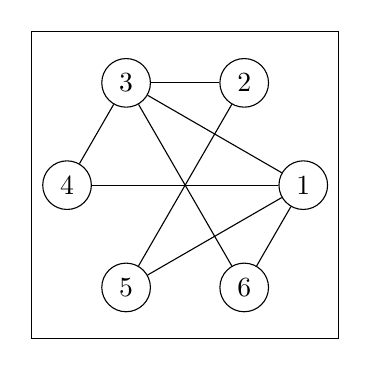
\begin{tikzpicture}
\tikzset{tinoeud/.style={draw, circle, minimum height=0.01cm}}
\clip (-2, -2) rectangle (2, 2);
\draw (-1.95, -1.95) rectangle (1.95, 1.95);
\node[tinoeud] (V1) at (0:1.5cm) {1};
\node[tinoeud] (V2) at (60:1.5cm) {2};
\node[tinoeud] (V3) at (120:1.5cm) {3};
\node[tinoeud] (V4) at (180:1.5cm) {4};
\node[tinoeud] (V5) at (240:1.5cm) {5};
\node[tinoeud] (V6) at (300:1.5cm) {6};
\draw (V1) -- (V3);
\draw (V1) -- (V4);
\draw (V1) -- (V5);
\draw (V1) -- (V6);
\draw (V2) -- (V3);
\draw (V2) -- (V5);
\draw (V3) -- (V4);
\draw (V3) -- (V6);
\end{tikzpicture}
\\
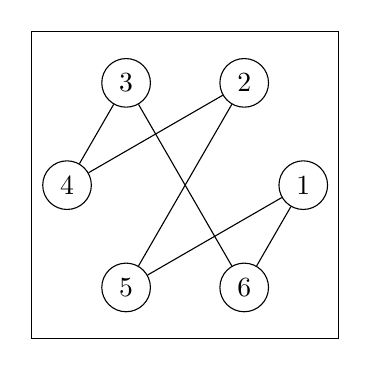
\begin{tikzpicture}
\tikzset{tinoeud/.style={draw, circle, minimum height=0.01cm}}
\clip (-2, -2) rectangle (2, 2);
\draw (-1.95, -1.95) rectangle (1.95, 1.95);
\node[tinoeud] (V1) at (0:1.5cm) {1};
\node[tinoeud] (V2) at (60:1.5cm) {2};
\node[tinoeud] (V3) at (120:1.5cm) {3};
\node[tinoeud] (V4) at (180:1.5cm) {4};
\node[tinoeud] (V5) at (240:1.5cm) {5};
\node[tinoeud] (V6) at (300:1.5cm) {6};
\draw (V1) -- (V5);
\draw (V1) -- (V6);
\draw (V2) -- (V4);
\draw (V2) -- (V5);
\draw (V3) -- (V4);
\draw (V3) -- (V6);
\end{tikzpicture}
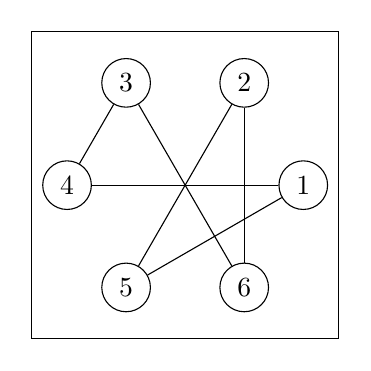
\begin{tikzpicture}
\tikzset{tinoeud/.style={draw, circle, minimum height=0.01cm}}
\clip (-2, -2) rectangle (2, 2);
\draw (-1.95, -1.95) rectangle (1.95, 1.95);
\node[tinoeud] (V1) at (0:1.5cm) {1};
\node[tinoeud] (V2) at (60:1.5cm) {2};
\node[tinoeud] (V3) at (120:1.5cm) {3};
\node[tinoeud] (V4) at (180:1.5cm) {4};
\node[tinoeud] (V5) at (240:1.5cm) {5};
\node[tinoeud] (V6) at (300:1.5cm) {6};
\draw (V1) -- (V4);
\draw (V1) -- (V5);
\draw (V2) -- (V5);
\draw (V2) -- (V6);
\draw (V3) -- (V4);
\draw (V3) -- (V6);
\end{tikzpicture}
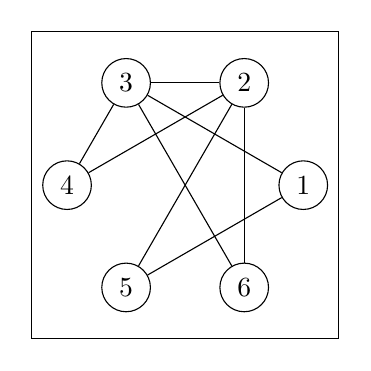
\begin{tikzpicture}
\tikzset{tinoeud/.style={draw, circle, minimum height=0.01cm}}
\clip (-2, -2) rectangle (2, 2);
\draw (-1.95, -1.95) rectangle (1.95, 1.95);
\node[tinoeud] (V1) at (0:1.5cm) {1};
\node[tinoeud] (V2) at (60:1.5cm) {2};
\node[tinoeud] (V3) at (120:1.5cm) {3};
\node[tinoeud] (V4) at (180:1.5cm) {4};
\node[tinoeud] (V5) at (240:1.5cm) {5};
\node[tinoeud] (V6) at (300:1.5cm) {6};
\draw (V1) -- (V3);
\draw (V1) -- (V5);
\draw (V2) -- (V3);
\draw (V2) -- (V4);
\draw (V2) -- (V5);
\draw (V2) -- (V6);
\draw (V3) -- (V4);
\draw (V3) -- (V6);
\end{tikzpicture}
\\
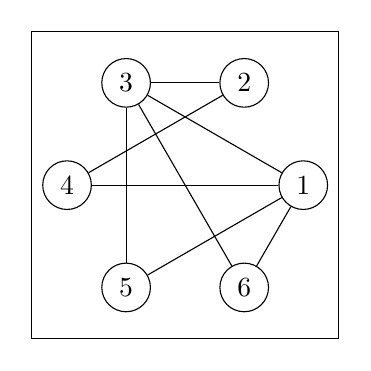
\begin{tikzpicture}
\tikzset{tinoeud/.style={draw, circle, minimum height=0.01cm}}
\clip (-2, -2) rectangle (2, 2);
\draw (-1.95, -1.95) rectangle (1.95, 1.95);
\node[tinoeud] (V1) at (0:1.5cm) {1};
\node[tinoeud] (V2) at (60:1.5cm) {2};
\node[tinoeud] (V3) at (120:1.5cm) {3};
\node[tinoeud] (V4) at (180:1.5cm) {4};
\node[tinoeud] (V5) at (240:1.5cm) {5};
\node[tinoeud] (V6) at (300:1.5cm) {6};
\draw (V1) -- (V3);
\draw (V1) -- (V4);
\draw (V1) -- (V5);
\draw (V1) -- (V6);
\draw (V2) -- (V3);
\draw (V2) -- (V4);
\draw (V3) -- (V5);
\draw (V3) -- (V6);
\end{tikzpicture}
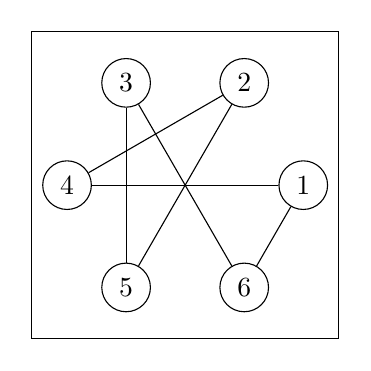
\begin{tikzpicture}
\tikzset{tinoeud/.style={draw, circle, minimum height=0.01cm}}
\clip (-2, -2) rectangle (2, 2);
\draw (-1.95, -1.95) rectangle (1.95, 1.95);
\node[tinoeud] (V1) at (0:1.5cm) {1};
\node[tinoeud] (V2) at (60:1.5cm) {2};
\node[tinoeud] (V3) at (120:1.5cm) {3};
\node[tinoeud] (V4) at (180:1.5cm) {4};
\node[tinoeud] (V5) at (240:1.5cm) {5};
\node[tinoeud] (V6) at (300:1.5cm) {6};
\draw (V1) -- (V4);
\draw (V1) -- (V6);
\draw (V2) -- (V4);
\draw (V2) -- (V5);
\draw (V3) -- (V5);
\draw (V3) -- (V6);
\end{tikzpicture}
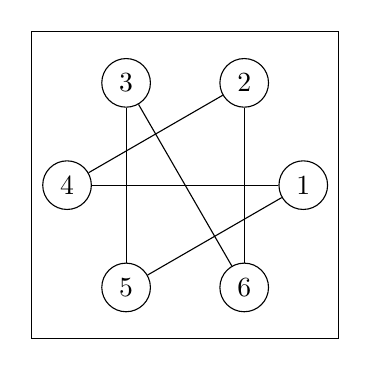
\begin{tikzpicture}
\tikzset{tinoeud/.style={draw, circle, minimum height=0.01cm}}
\clip (-2, -2) rectangle (2, 2);
\draw (-1.95, -1.95) rectangle (1.95, 1.95);
\node[tinoeud] (V1) at (0:1.5cm) {1};
\node[tinoeud] (V2) at (60:1.5cm) {2};
\node[tinoeud] (V3) at (120:1.5cm) {3};
\node[tinoeud] (V4) at (180:1.5cm) {4};
\node[tinoeud] (V5) at (240:1.5cm) {5};
\node[tinoeud] (V6) at (300:1.5cm) {6};
\draw (V1) -- (V4);
\draw (V1) -- (V5);
\draw (V2) -- (V4);
\draw (V2) -- (V6);
\draw (V3) -- (V5);
\draw (V3) -- (V6);
\end{tikzpicture}
\\
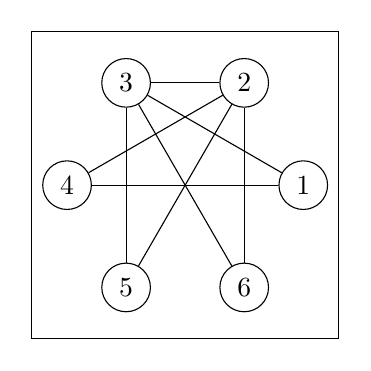
\begin{tikzpicture}
\tikzset{tinoeud/.style={draw, circle, minimum height=0.01cm}}
\clip (-2, -2) rectangle (2, 2);
\draw (-1.95, -1.95) rectangle (1.95, 1.95);
\node[tinoeud] (V1) at (0:1.5cm) {1};
\node[tinoeud] (V2) at (60:1.5cm) {2};
\node[tinoeud] (V3) at (120:1.5cm) {3};
\node[tinoeud] (V4) at (180:1.5cm) {4};
\node[tinoeud] (V5) at (240:1.5cm) {5};
\node[tinoeud] (V6) at (300:1.5cm) {6};
\draw (V1) -- (V3);
\draw (V1) -- (V4);
\draw (V2) -- (V3);
\draw (V2) -- (V4);
\draw (V2) -- (V5);
\draw (V2) -- (V6);
\draw (V3) -- (V5);
\draw (V3) -- (V6);
\end{tikzpicture}
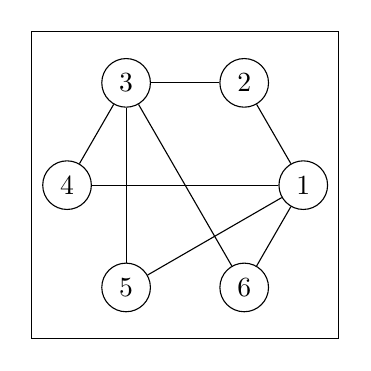
\begin{tikzpicture}
\tikzset{tinoeud/.style={draw, circle, minimum height=0.01cm}}
\clip (-2, -2) rectangle (2, 2);
\draw (-1.95, -1.95) rectangle (1.95, 1.95);
\node[tinoeud] (V1) at (0:1.5cm) {1};
\node[tinoeud] (V2) at (60:1.5cm) {2};
\node[tinoeud] (V3) at (120:1.5cm) {3};
\node[tinoeud] (V4) at (180:1.5cm) {4};
\node[tinoeud] (V5) at (240:1.5cm) {5};
\node[tinoeud] (V6) at (300:1.5cm) {6};
\draw (V1) -- (V2);
\draw (V1) -- (V4);
\draw (V1) -- (V5);
\draw (V1) -- (V6);
\draw (V2) -- (V3);
\draw (V3) -- (V4);
\draw (V3) -- (V5);
\draw (V3) -- (V6);
\end{tikzpicture}
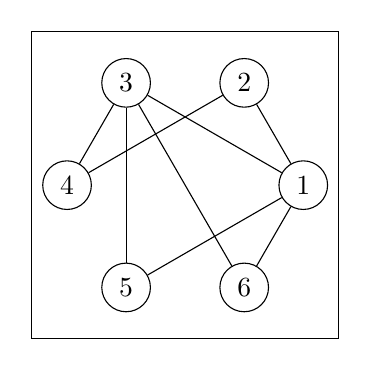
\begin{tikzpicture}
\tikzset{tinoeud/.style={draw, circle, minimum height=0.01cm}}
\clip (-2, -2) rectangle (2, 2);
\draw (-1.95, -1.95) rectangle (1.95, 1.95);
\node[tinoeud] (V1) at (0:1.5cm) {1};
\node[tinoeud] (V2) at (60:1.5cm) {2};
\node[tinoeud] (V3) at (120:1.5cm) {3};
\node[tinoeud] (V4) at (180:1.5cm) {4};
\node[tinoeud] (V5) at (240:1.5cm) {5};
\node[tinoeud] (V6) at (300:1.5cm) {6};
\draw (V1) -- (V2);
\draw (V1) -- (V3);
\draw (V1) -- (V5);
\draw (V1) -- (V6);
\draw (V2) -- (V4);
\draw (V3) -- (V4);
\draw (V3) -- (V5);
\draw (V3) -- (V6);
\end{tikzpicture}
\\
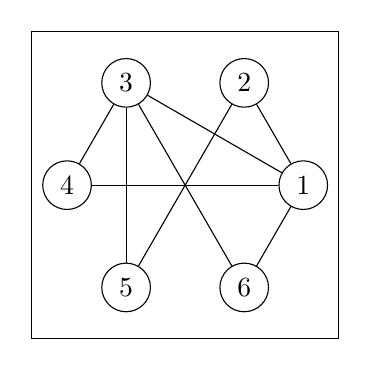
\begin{tikzpicture}
\tikzset{tinoeud/.style={draw, circle, minimum height=0.01cm}}
\clip (-2, -2) rectangle (2, 2);
\draw (-1.95, -1.95) rectangle (1.95, 1.95);
\node[tinoeud] (V1) at (0:1.5cm) {1};
\node[tinoeud] (V2) at (60:1.5cm) {2};
\node[tinoeud] (V3) at (120:1.5cm) {3};
\node[tinoeud] (V4) at (180:1.5cm) {4};
\node[tinoeud] (V5) at (240:1.5cm) {5};
\node[tinoeud] (V6) at (300:1.5cm) {6};
\draw (V1) -- (V2);
\draw (V1) -- (V3);
\draw (V1) -- (V4);
\draw (V1) -- (V6);
\draw (V2) -- (V5);
\draw (V3) -- (V4);
\draw (V3) -- (V5);
\draw (V3) -- (V6);
\end{tikzpicture}
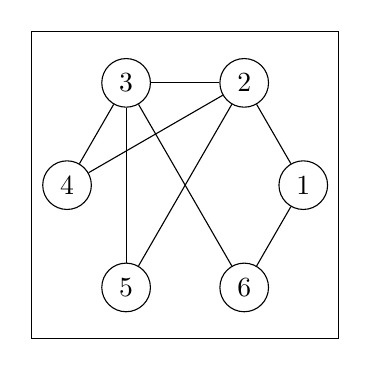
\begin{tikzpicture}
\tikzset{tinoeud/.style={draw, circle, minimum height=0.01cm}}
\clip (-2, -2) rectangle (2, 2);
\draw (-1.95, -1.95) rectangle (1.95, 1.95);
\node[tinoeud] (V1) at (0:1.5cm) {1};
\node[tinoeud] (V2) at (60:1.5cm) {2};
\node[tinoeud] (V3) at (120:1.5cm) {3};
\node[tinoeud] (V4) at (180:1.5cm) {4};
\node[tinoeud] (V5) at (240:1.5cm) {5};
\node[tinoeud] (V6) at (300:1.5cm) {6};
\draw (V1) -- (V2);
\draw (V1) -- (V6);
\draw (V2) -- (V3);
\draw (V2) -- (V4);
\draw (V2) -- (V5);
\draw (V3) -- (V4);
\draw (V3) -- (V5);
\draw (V3) -- (V6);
\end{tikzpicture}
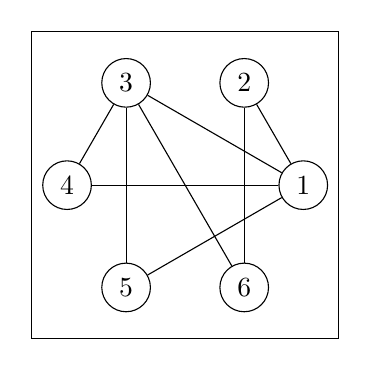
\begin{tikzpicture}
\tikzset{tinoeud/.style={draw, circle, minimum height=0.01cm}}
\clip (-2, -2) rectangle (2, 2);
\draw (-1.95, -1.95) rectangle (1.95, 1.95);
\node[tinoeud] (V1) at (0:1.5cm) {1};
\node[tinoeud] (V2) at (60:1.5cm) {2};
\node[tinoeud] (V3) at (120:1.5cm) {3};
\node[tinoeud] (V4) at (180:1.5cm) {4};
\node[tinoeud] (V5) at (240:1.5cm) {5};
\node[tinoeud] (V6) at (300:1.5cm) {6};
\draw (V1) -- (V2);
\draw (V1) -- (V3);
\draw (V1) -- (V4);
\draw (V1) -- (V5);
\draw (V2) -- (V6);
\draw (V3) -- (V4);
\draw (V3) -- (V5);
\draw (V3) -- (V6);
\end{tikzpicture}
\\
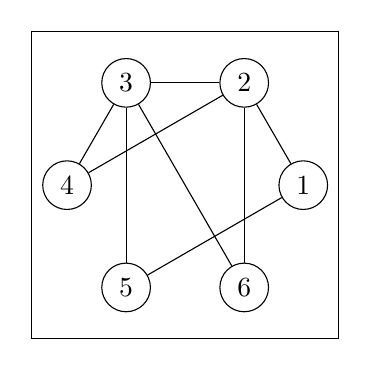
\begin{tikzpicture}
\tikzset{tinoeud/.style={draw, circle, minimum height=0.01cm}}
\clip (-2, -2) rectangle (2, 2);
\draw (-1.95, -1.95) rectangle (1.95, 1.95);
\node[tinoeud] (V1) at (0:1.5cm) {1};
\node[tinoeud] (V2) at (60:1.5cm) {2};
\node[tinoeud] (V3) at (120:1.5cm) {3};
\node[tinoeud] (V4) at (180:1.5cm) {4};
\node[tinoeud] (V5) at (240:1.5cm) {5};
\node[tinoeud] (V6) at (300:1.5cm) {6};
\draw (V1) -- (V2);
\draw (V1) -- (V5);
\draw (V2) -- (V3);
\draw (V2) -- (V4);
\draw (V2) -- (V6);
\draw (V3) -- (V4);
\draw (V3) -- (V5);
\draw (V3) -- (V6);
\end{tikzpicture}
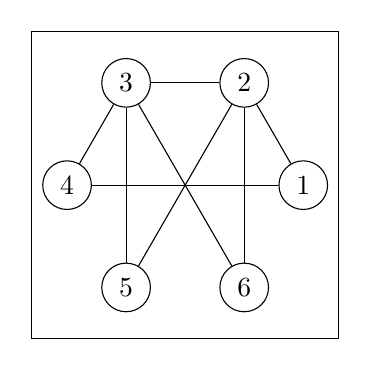
\begin{tikzpicture}
\tikzset{tinoeud/.style={draw, circle, minimum height=0.01cm}}
\clip (-2, -2) rectangle (2, 2);
\draw (-1.95, -1.95) rectangle (1.95, 1.95);
\node[tinoeud] (V1) at (0:1.5cm) {1};
\node[tinoeud] (V2) at (60:1.5cm) {2};
\node[tinoeud] (V3) at (120:1.5cm) {3};
\node[tinoeud] (V4) at (180:1.5cm) {4};
\node[tinoeud] (V5) at (240:1.5cm) {5};
\node[tinoeud] (V6) at (300:1.5cm) {6};
\draw (V1) -- (V2);
\draw (V1) -- (V4);
\draw (V2) -- (V3);
\draw (V2) -- (V5);
\draw (V2) -- (V6);
\draw (V3) -- (V4);
\draw (V3) -- (V5);
\draw (V3) -- (V6);
\end{tikzpicture}
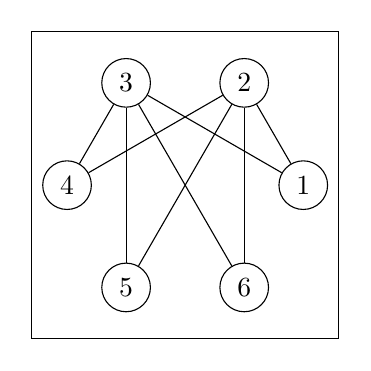
\begin{tikzpicture}
\tikzset{tinoeud/.style={draw, circle, minimum height=0.01cm}}
\clip (-2, -2) rectangle (2, 2);
\draw (-1.95, -1.95) rectangle (1.95, 1.95);
\node[tinoeud] (V1) at (0:1.5cm) {1};
\node[tinoeud] (V2) at (60:1.5cm) {2};
\node[tinoeud] (V3) at (120:1.5cm) {3};
\node[tinoeud] (V4) at (180:1.5cm) {4};
\node[tinoeud] (V5) at (240:1.5cm) {5};
\node[tinoeud] (V6) at (300:1.5cm) {6};
\draw (V1) -- (V2);
\draw (V1) -- (V3);
\draw (V2) -- (V4);
\draw (V2) -- (V5);
\draw (V2) -- (V6);
\draw (V3) -- (V4);
\draw (V3) -- (V5);
\draw (V3) -- (V6);
\end{tikzpicture}
\\
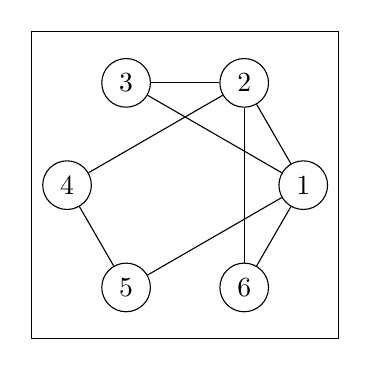
\begin{tikzpicture}
\tikzset{tinoeud/.style={draw, circle, minimum height=0.01cm}}
\clip (-2, -2) rectangle (2, 2);
\draw (-1.95, -1.95) rectangle (1.95, 1.95);
\node[tinoeud] (V1) at (0:1.5cm) {1};
\node[tinoeud] (V2) at (60:1.5cm) {2};
\node[tinoeud] (V3) at (120:1.5cm) {3};
\node[tinoeud] (V4) at (180:1.5cm) {4};
\node[tinoeud] (V5) at (240:1.5cm) {5};
\node[tinoeud] (V6) at (300:1.5cm) {6};
\draw (V1) -- (V2);
\draw (V1) -- (V3);
\draw (V1) -- (V5);
\draw (V1) -- (V6);
\draw (V2) -- (V3);
\draw (V2) -- (V4);
\draw (V2) -- (V6);
\draw (V4) -- (V5);
\end{tikzpicture}
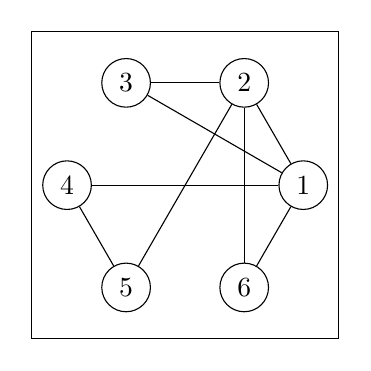
\begin{tikzpicture}
\tikzset{tinoeud/.style={draw, circle, minimum height=0.01cm}}
\clip (-2, -2) rectangle (2, 2);
\draw (-1.95, -1.95) rectangle (1.95, 1.95);
\node[tinoeud] (V1) at (0:1.5cm) {1};
\node[tinoeud] (V2) at (60:1.5cm) {2};
\node[tinoeud] (V3) at (120:1.5cm) {3};
\node[tinoeud] (V4) at (180:1.5cm) {4};
\node[tinoeud] (V5) at (240:1.5cm) {5};
\node[tinoeud] (V6) at (300:1.5cm) {6};
\draw (V1) -- (V2);
\draw (V1) -- (V3);
\draw (V1) -- (V4);
\draw (V1) -- (V6);
\draw (V2) -- (V3);
\draw (V2) -- (V5);
\draw (V2) -- (V6);
\draw (V4) -- (V5);
\end{tikzpicture}
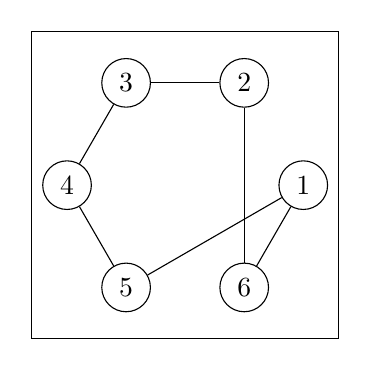
\begin{tikzpicture}
\tikzset{tinoeud/.style={draw, circle, minimum height=0.01cm}}
\clip (-2, -2) rectangle (2, 2);
\draw (-1.95, -1.95) rectangle (1.95, 1.95);
\node[tinoeud] (V1) at (0:1.5cm) {1};
\node[tinoeud] (V2) at (60:1.5cm) {2};
\node[tinoeud] (V3) at (120:1.5cm) {3};
\node[tinoeud] (V4) at (180:1.5cm) {4};
\node[tinoeud] (V5) at (240:1.5cm) {5};
\node[tinoeud] (V6) at (300:1.5cm) {6};
\draw (V1) -- (V5);
\draw (V1) -- (V6);
\draw (V2) -- (V3);
\draw (V2) -- (V6);
\draw (V3) -- (V4);
\draw (V4) -- (V5);
\end{tikzpicture}
\\
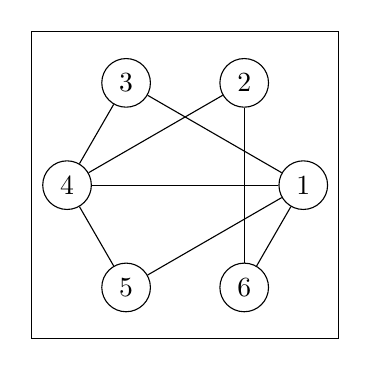
\begin{tikzpicture}
\tikzset{tinoeud/.style={draw, circle, minimum height=0.01cm}}
\clip (-2, -2) rectangle (2, 2);
\draw (-1.95, -1.95) rectangle (1.95, 1.95);
\node[tinoeud] (V1) at (0:1.5cm) {1};
\node[tinoeud] (V2) at (60:1.5cm) {2};
\node[tinoeud] (V3) at (120:1.5cm) {3};
\node[tinoeud] (V4) at (180:1.5cm) {4};
\node[tinoeud] (V5) at (240:1.5cm) {5};
\node[tinoeud] (V6) at (300:1.5cm) {6};
\draw (V1) -- (V3);
\draw (V1) -- (V4);
\draw (V1) -- (V5);
\draw (V1) -- (V6);
\draw (V2) -- (V4);
\draw (V2) -- (V6);
\draw (V3) -- (V4);
\draw (V4) -- (V5);
\end{tikzpicture}
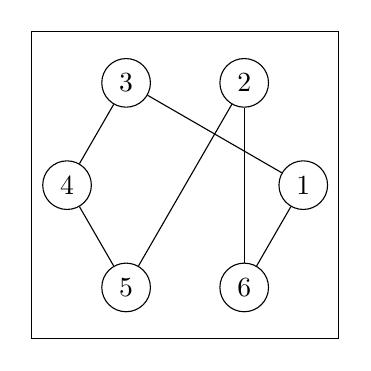
\begin{tikzpicture}
\tikzset{tinoeud/.style={draw, circle, minimum height=0.01cm}}
\clip (-2, -2) rectangle (2, 2);
\draw (-1.95, -1.95) rectangle (1.95, 1.95);
\node[tinoeud] (V1) at (0:1.5cm) {1};
\node[tinoeud] (V2) at (60:1.5cm) {2};
\node[tinoeud] (V3) at (120:1.5cm) {3};
\node[tinoeud] (V4) at (180:1.5cm) {4};
\node[tinoeud] (V5) at (240:1.5cm) {5};
\node[tinoeud] (V6) at (300:1.5cm) {6};
\draw (V1) -- (V3);
\draw (V1) -- (V6);
\draw (V2) -- (V5);
\draw (V2) -- (V6);
\draw (V3) -- (V4);
\draw (V4) -- (V5);
\end{tikzpicture}
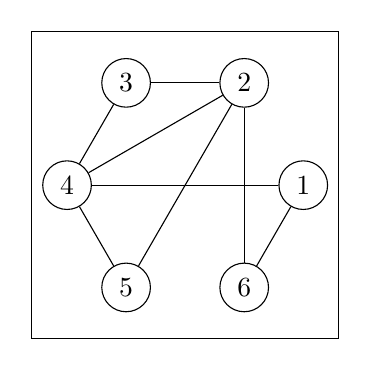
\begin{tikzpicture}
\tikzset{tinoeud/.style={draw, circle, minimum height=0.01cm}}
\clip (-2, -2) rectangle (2, 2);
\draw (-1.95, -1.95) rectangle (1.95, 1.95);
\node[tinoeud] (V1) at (0:1.5cm) {1};
\node[tinoeud] (V2) at (60:1.5cm) {2};
\node[tinoeud] (V3) at (120:1.5cm) {3};
\node[tinoeud] (V4) at (180:1.5cm) {4};
\node[tinoeud] (V5) at (240:1.5cm) {5};
\node[tinoeud] (V6) at (300:1.5cm) {6};
\draw (V1) -- (V4);
\draw (V1) -- (V6);
\draw (V2) -- (V3);
\draw (V2) -- (V4);
\draw (V2) -- (V5);
\draw (V2) -- (V6);
\draw (V3) -- (V4);
\draw (V4) -- (V5);
\end{tikzpicture}
\\
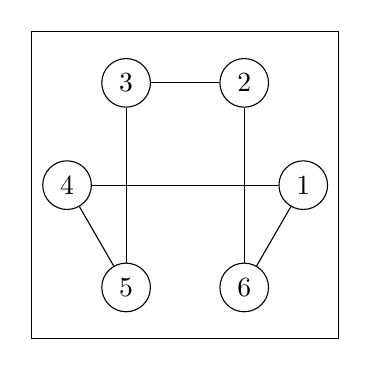
\begin{tikzpicture}
\tikzset{tinoeud/.style={draw, circle, minimum height=0.01cm}}
\clip (-2, -2) rectangle (2, 2);
\draw (-1.95, -1.95) rectangle (1.95, 1.95);
\node[tinoeud] (V1) at (0:1.5cm) {1};
\node[tinoeud] (V2) at (60:1.5cm) {2};
\node[tinoeud] (V3) at (120:1.5cm) {3};
\node[tinoeud] (V4) at (180:1.5cm) {4};
\node[tinoeud] (V5) at (240:1.5cm) {5};
\node[tinoeud] (V6) at (300:1.5cm) {6};
\draw (V1) -- (V4);
\draw (V1) -- (V6);
\draw (V2) -- (V3);
\draw (V2) -- (V6);
\draw (V3) -- (V5);
\draw (V4) -- (V5);
\end{tikzpicture}
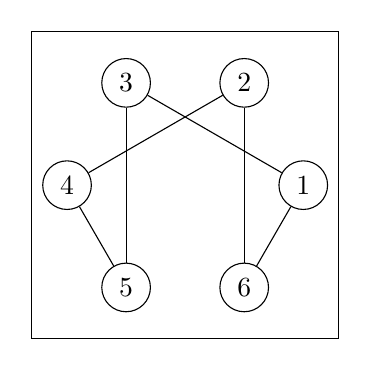
\begin{tikzpicture}
\tikzset{tinoeud/.style={draw, circle, minimum height=0.01cm}}
\clip (-2, -2) rectangle (2, 2);
\draw (-1.95, -1.95) rectangle (1.95, 1.95);
\node[tinoeud] (V1) at (0:1.5cm) {1};
\node[tinoeud] (V2) at (60:1.5cm) {2};
\node[tinoeud] (V3) at (120:1.5cm) {3};
\node[tinoeud] (V4) at (180:1.5cm) {4};
\node[tinoeud] (V5) at (240:1.5cm) {5};
\node[tinoeud] (V6) at (300:1.5cm) {6};
\draw (V1) -- (V3);
\draw (V1) -- (V6);
\draw (V2) -- (V4);
\draw (V2) -- (V6);
\draw (V3) -- (V5);
\draw (V4) -- (V5);
\end{tikzpicture}
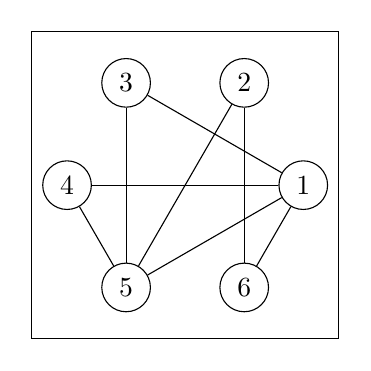
\begin{tikzpicture}
\tikzset{tinoeud/.style={draw, circle, minimum height=0.01cm}}
\clip (-2, -2) rectangle (2, 2);
\draw (-1.95, -1.95) rectangle (1.95, 1.95);
\node[tinoeud] (V1) at (0:1.5cm) {1};
\node[tinoeud] (V2) at (60:1.5cm) {2};
\node[tinoeud] (V3) at (120:1.5cm) {3};
\node[tinoeud] (V4) at (180:1.5cm) {4};
\node[tinoeud] (V5) at (240:1.5cm) {5};
\node[tinoeud] (V6) at (300:1.5cm) {6};
\draw (V1) -- (V3);
\draw (V1) -- (V4);
\draw (V1) -- (V5);
\draw (V1) -- (V6);
\draw (V2) -- (V5);
\draw (V2) -- (V6);
\draw (V3) -- (V5);
\draw (V4) -- (V5);
\end{tikzpicture}
\\
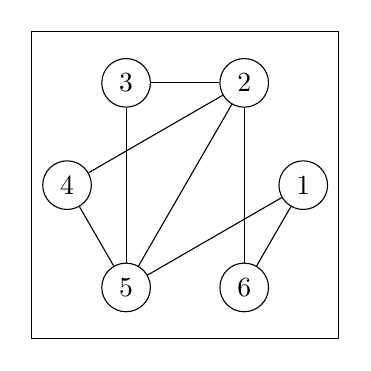
\begin{tikzpicture}
\tikzset{tinoeud/.style={draw, circle, minimum height=0.01cm}}
\clip (-2, -2) rectangle (2, 2);
\draw (-1.95, -1.95) rectangle (1.95, 1.95);
\node[tinoeud] (V1) at (0:1.5cm) {1};
\node[tinoeud] (V2) at (60:1.5cm) {2};
\node[tinoeud] (V3) at (120:1.5cm) {3};
\node[tinoeud] (V4) at (180:1.5cm) {4};
\node[tinoeud] (V5) at (240:1.5cm) {5};
\node[tinoeud] (V6) at (300:1.5cm) {6};
\draw (V1) -- (V5);
\draw (V1) -- (V6);
\draw (V2) -- (V3);
\draw (V2) -- (V4);
\draw (V2) -- (V5);
\draw (V2) -- (V6);
\draw (V3) -- (V5);
\draw (V4) -- (V5);
\end{tikzpicture}
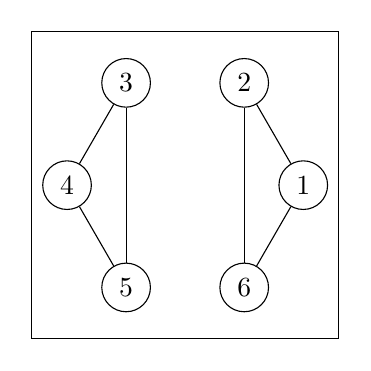
\begin{tikzpicture}
\tikzset{tinoeud/.style={draw, circle, minimum height=0.01cm}}
\clip (-2, -2) rectangle (2, 2);
\draw (-1.95, -1.95) rectangle (1.95, 1.95);
\node[tinoeud] (V1) at (0:1.5cm) {1};
\node[tinoeud] (V2) at (60:1.5cm) {2};
\node[tinoeud] (V3) at (120:1.5cm) {3};
\node[tinoeud] (V4) at (180:1.5cm) {4};
\node[tinoeud] (V5) at (240:1.5cm) {5};
\node[tinoeud] (V6) at (300:1.5cm) {6};
\draw (V1) -- (V2);
\draw (V1) -- (V6);
\draw (V2) -- (V6);
\draw (V3) -- (V4);
\draw (V3) -- (V5);
\draw (V4) -- (V5);
\end{tikzpicture}
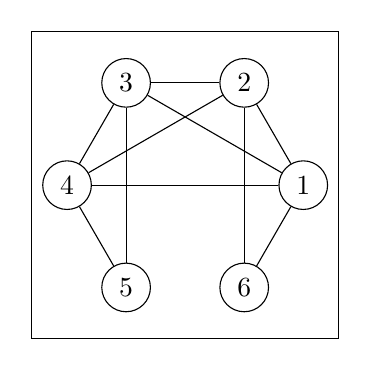
\begin{tikzpicture}
\tikzset{tinoeud/.style={draw, circle, minimum height=0.01cm}}
\clip (-2, -2) rectangle (2, 2);
\draw (-1.95, -1.95) rectangle (1.95, 1.95);
\node[tinoeud] (V1) at (0:1.5cm) {1};
\node[tinoeud] (V2) at (60:1.5cm) {2};
\node[tinoeud] (V3) at (120:1.5cm) {3};
\node[tinoeud] (V4) at (180:1.5cm) {4};
\node[tinoeud] (V5) at (240:1.5cm) {5};
\node[tinoeud] (V6) at (300:1.5cm) {6};
\draw (V1) -- (V2);
\draw (V1) -- (V3);
\draw (V1) -- (V4);
\draw (V1) -- (V6);
\draw (V2) -- (V3);
\draw (V2) -- (V4);
\draw (V2) -- (V6);
\draw (V3) -- (V4);
\draw (V3) -- (V5);
\draw (V4) -- (V5);
\end{tikzpicture}
\\
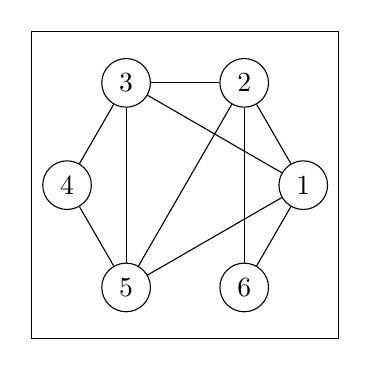
\begin{tikzpicture}
\tikzset{tinoeud/.style={draw, circle, minimum height=0.01cm}}
\clip (-2, -2) rectangle (2, 2);
\draw (-1.95, -1.95) rectangle (1.95, 1.95);
\node[tinoeud] (V1) at (0:1.5cm) {1};
\node[tinoeud] (V2) at (60:1.5cm) {2};
\node[tinoeud] (V3) at (120:1.5cm) {3};
\node[tinoeud] (V4) at (180:1.5cm) {4};
\node[tinoeud] (V5) at (240:1.5cm) {5};
\node[tinoeud] (V6) at (300:1.5cm) {6};
\draw (V1) -- (V2);
\draw (V1) -- (V3);
\draw (V1) -- (V5);
\draw (V1) -- (V6);
\draw (V2) -- (V3);
\draw (V2) -- (V5);
\draw (V2) -- (V6);
\draw (V3) -- (V4);
\draw (V3) -- (V5);
\draw (V4) -- (V5);
\end{tikzpicture}
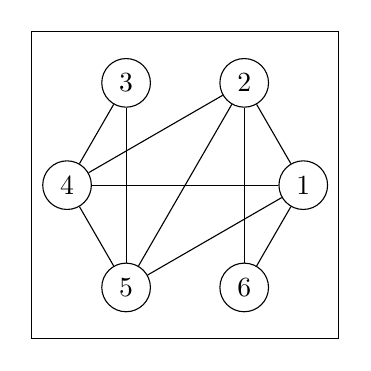
\begin{tikzpicture}
\tikzset{tinoeud/.style={draw, circle, minimum height=0.01cm}}
\clip (-2, -2) rectangle (2, 2);
\draw (-1.95, -1.95) rectangle (1.95, 1.95);
\node[tinoeud] (V1) at (0:1.5cm) {1};
\node[tinoeud] (V2) at (60:1.5cm) {2};
\node[tinoeud] (V3) at (120:1.5cm) {3};
\node[tinoeud] (V4) at (180:1.5cm) {4};
\node[tinoeud] (V5) at (240:1.5cm) {5};
\node[tinoeud] (V6) at (300:1.5cm) {6};
\draw (V1) -- (V2);
\draw (V1) -- (V4);
\draw (V1) -- (V5);
\draw (V1) -- (V6);
\draw (V2) -- (V4);
\draw (V2) -- (V5);
\draw (V2) -- (V6);
\draw (V3) -- (V4);
\draw (V3) -- (V5);
\draw (V4) -- (V5);
\end{tikzpicture}
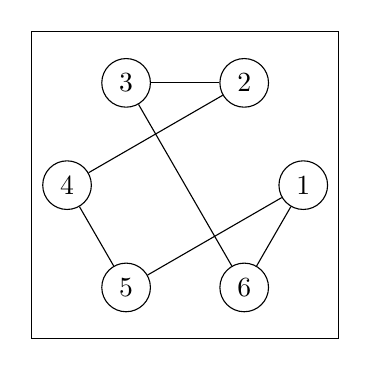
\begin{tikzpicture}
\tikzset{tinoeud/.style={draw, circle, minimum height=0.01cm}}
\clip (-2, -2) rectangle (2, 2);
\draw (-1.95, -1.95) rectangle (1.95, 1.95);
\node[tinoeud] (V1) at (0:1.5cm) {1};
\node[tinoeud] (V2) at (60:1.5cm) {2};
\node[tinoeud] (V3) at (120:1.5cm) {3};
\node[tinoeud] (V4) at (180:1.5cm) {4};
\node[tinoeud] (V5) at (240:1.5cm) {5};
\node[tinoeud] (V6) at (300:1.5cm) {6};
\draw (V1) -- (V5);
\draw (V1) -- (V6);
\draw (V2) -- (V3);
\draw (V2) -- (V4);
\draw (V3) -- (V6);
\draw (V4) -- (V5);
\end{tikzpicture}
\\
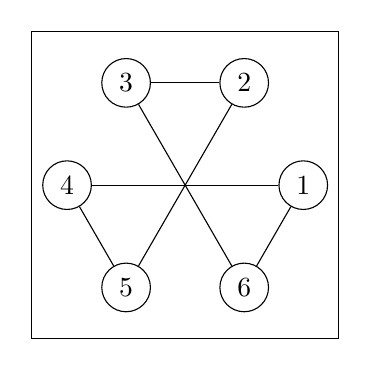
\begin{tikzpicture}
\tikzset{tinoeud/.style={draw, circle, minimum height=0.01cm}}
\clip (-2, -2) rectangle (2, 2);
\draw (-1.95, -1.95) rectangle (1.95, 1.95);
\node[tinoeud] (V1) at (0:1.5cm) {1};
\node[tinoeud] (V2) at (60:1.5cm) {2};
\node[tinoeud] (V3) at (120:1.5cm) {3};
\node[tinoeud] (V4) at (180:1.5cm) {4};
\node[tinoeud] (V5) at (240:1.5cm) {5};
\node[tinoeud] (V6) at (300:1.5cm) {6};
\draw (V1) -- (V4);
\draw (V1) -- (V6);
\draw (V2) -- (V3);
\draw (V2) -- (V5);
\draw (V3) -- (V6);
\draw (V4) -- (V5);
\end{tikzpicture}
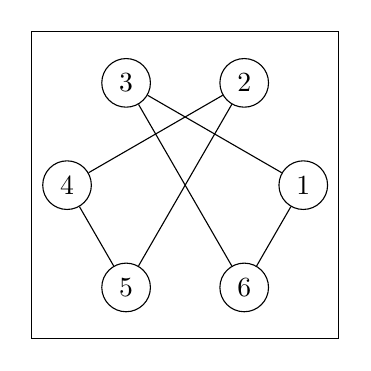
\begin{tikzpicture}
\tikzset{tinoeud/.style={draw, circle, minimum height=0.01cm}}
\clip (-2, -2) rectangle (2, 2);
\draw (-1.95, -1.95) rectangle (1.95, 1.95);
\node[tinoeud] (V1) at (0:1.5cm) {1};
\node[tinoeud] (V2) at (60:1.5cm) {2};
\node[tinoeud] (V3) at (120:1.5cm) {3};
\node[tinoeud] (V4) at (180:1.5cm) {4};
\node[tinoeud] (V5) at (240:1.5cm) {5};
\node[tinoeud] (V6) at (300:1.5cm) {6};
\draw (V1) -- (V3);
\draw (V1) -- (V6);
\draw (V2) -- (V4);
\draw (V2) -- (V5);
\draw (V3) -- (V6);
\draw (V4) -- (V5);
\end{tikzpicture}
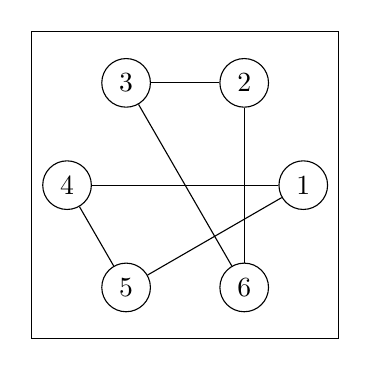
\begin{tikzpicture}
\tikzset{tinoeud/.style={draw, circle, minimum height=0.01cm}}
\clip (-2, -2) rectangle (2, 2);
\draw (-1.95, -1.95) rectangle (1.95, 1.95);
\node[tinoeud] (V1) at (0:1.5cm) {1};
\node[tinoeud] (V2) at (60:1.5cm) {2};
\node[tinoeud] (V3) at (120:1.5cm) {3};
\node[tinoeud] (V4) at (180:1.5cm) {4};
\node[tinoeud] (V5) at (240:1.5cm) {5};
\node[tinoeud] (V6) at (300:1.5cm) {6};
\draw (V1) -- (V4);
\draw (V1) -- (V5);
\draw (V2) -- (V3);
\draw (V2) -- (V6);
\draw (V3) -- (V6);
\draw (V4) -- (V5);
\end{tikzpicture}
\\
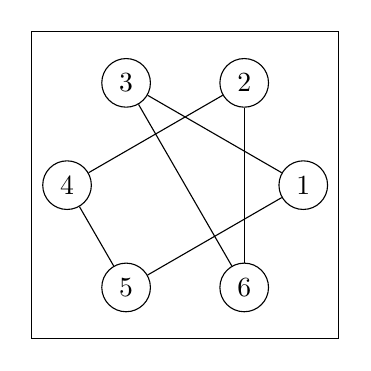
\begin{tikzpicture}
\tikzset{tinoeud/.style={draw, circle, minimum height=0.01cm}}
\clip (-2, -2) rectangle (2, 2);
\draw (-1.95, -1.95) rectangle (1.95, 1.95);
\node[tinoeud] (V1) at (0:1.5cm) {1};
\node[tinoeud] (V2) at (60:1.5cm) {2};
\node[tinoeud] (V3) at (120:1.5cm) {3};
\node[tinoeud] (V4) at (180:1.5cm) {4};
\node[tinoeud] (V5) at (240:1.5cm) {5};
\node[tinoeud] (V6) at (300:1.5cm) {6};
\draw (V1) -- (V3);
\draw (V1) -- (V5);
\draw (V2) -- (V4);
\draw (V2) -- (V6);
\draw (V3) -- (V6);
\draw (V4) -- (V5);
\end{tikzpicture}
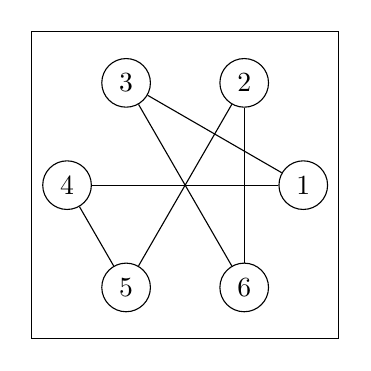
\begin{tikzpicture}
\tikzset{tinoeud/.style={draw, circle, minimum height=0.01cm}}
\clip (-2, -2) rectangle (2, 2);
\draw (-1.95, -1.95) rectangle (1.95, 1.95);
\node[tinoeud] (V1) at (0:1.5cm) {1};
\node[tinoeud] (V2) at (60:1.5cm) {2};
\node[tinoeud] (V3) at (120:1.5cm) {3};
\node[tinoeud] (V4) at (180:1.5cm) {4};
\node[tinoeud] (V5) at (240:1.5cm) {5};
\node[tinoeud] (V6) at (300:1.5cm) {6};
\draw (V1) -- (V3);
\draw (V1) -- (V4);
\draw (V2) -- (V5);
\draw (V2) -- (V6);
\draw (V3) -- (V6);
\draw (V4) -- (V5);
\end{tikzpicture}
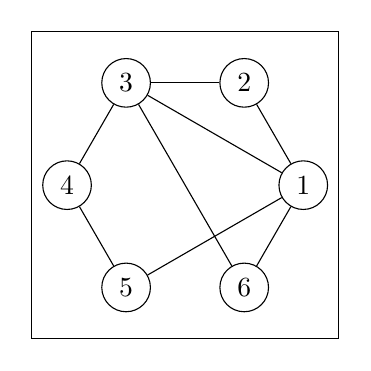
\begin{tikzpicture}
\tikzset{tinoeud/.style={draw, circle, minimum height=0.01cm}}
\clip (-2, -2) rectangle (2, 2);
\draw (-1.95, -1.95) rectangle (1.95, 1.95);
\node[tinoeud] (V1) at (0:1.5cm) {1};
\node[tinoeud] (V2) at (60:1.5cm) {2};
\node[tinoeud] (V3) at (120:1.5cm) {3};
\node[tinoeud] (V4) at (180:1.5cm) {4};
\node[tinoeud] (V5) at (240:1.5cm) {5};
\node[tinoeud] (V6) at (300:1.5cm) {6};
\draw (V1) -- (V2);
\draw (V1) -- (V3);
\draw (V1) -- (V5);
\draw (V1) -- (V6);
\draw (V2) -- (V3);
\draw (V3) -- (V4);
\draw (V3) -- (V6);
\draw (V4) -- (V5);
\end{tikzpicture}
\\
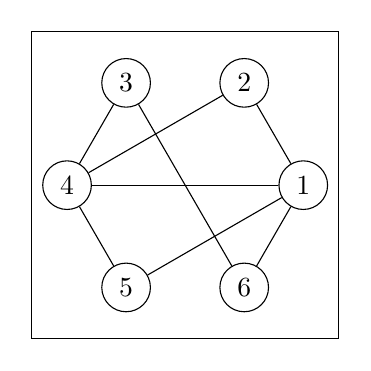
\begin{tikzpicture}
\tikzset{tinoeud/.style={draw, circle, minimum height=0.01cm}}
\clip (-2, -2) rectangle (2, 2);
\draw (-1.95, -1.95) rectangle (1.95, 1.95);
\node[tinoeud] (V1) at (0:1.5cm) {1};
\node[tinoeud] (V2) at (60:1.5cm) {2};
\node[tinoeud] (V3) at (120:1.5cm) {3};
\node[tinoeud] (V4) at (180:1.5cm) {4};
\node[tinoeud] (V5) at (240:1.5cm) {5};
\node[tinoeud] (V6) at (300:1.5cm) {6};
\draw (V1) -- (V2);
\draw (V1) -- (V4);
\draw (V1) -- (V5);
\draw (V1) -- (V6);
\draw (V2) -- (V4);
\draw (V3) -- (V4);
\draw (V3) -- (V6);
\draw (V4) -- (V5);
\end{tikzpicture}
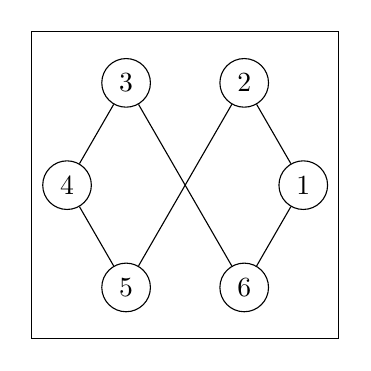
\begin{tikzpicture}
\tikzset{tinoeud/.style={draw, circle, minimum height=0.01cm}}
\clip (-2, -2) rectangle (2, 2);
\draw (-1.95, -1.95) rectangle (1.95, 1.95);
\node[tinoeud] (V1) at (0:1.5cm) {1};
\node[tinoeud] (V2) at (60:1.5cm) {2};
\node[tinoeud] (V3) at (120:1.5cm) {3};
\node[tinoeud] (V4) at (180:1.5cm) {4};
\node[tinoeud] (V5) at (240:1.5cm) {5};
\node[tinoeud] (V6) at (300:1.5cm) {6};
\draw (V1) -- (V2);
\draw (V1) -- (V6);
\draw (V2) -- (V5);
\draw (V3) -- (V4);
\draw (V3) -- (V6);
\draw (V4) -- (V5);
\end{tikzpicture}
\begin{tikzpicture}
\tikzset{tinoeud/.style={draw, circle, minimum height=0.01cm}}
\clip (-2, -2) rectangle (2, 2);
\draw (-1.95, -1.95) rectangle (1.95, 1.95);
\node[tinoeud] (V1) at (0:1.5cm) {1};
\node[tinoeud] (V2) at (60:1.5cm) {2};
\node[tinoeud] (V3) at (120:1.5cm) {3};
\node[tinoeud] (V4) at (180:1.5cm) {4};
\node[tinoeud] (V5) at (240:1.5cm) {5};
\node[tinoeud] (V6) at (300:1.5cm) {6};
\draw (V1) -- (V2);
\draw (V1) -- (V3);
\draw (V1) -- (V4);
\draw (V1) -- (V6);
\draw (V2) -- (V3);
\draw (V2) -- (V4);
\draw (V2) -- (V5);
\draw (V3) -- (V4);
\draw (V3) -- (V6);
\draw (V4) -- (V5);
\end{tikzpicture}
\\
\begin{tikzpicture}
\tikzset{tinoeud/.style={draw, circle, minimum height=0.01cm}}
\clip (-2, -2) rectangle (2, 2);
\draw (-1.95, -1.95) rectangle (1.95, 1.95);
\node[tinoeud] (V1) at (0:1.5cm) {1};
\node[tinoeud] (V2) at (60:1.5cm) {2};
\node[tinoeud] (V3) at (120:1.5cm) {3};
\node[tinoeud] (V4) at (180:1.5cm) {4};
\node[tinoeud] (V5) at (240:1.5cm) {5};
\node[tinoeud] (V6) at (300:1.5cm) {6};
\draw (V1) -- (V2);
\draw (V1) -- (V5);
\draw (V2) -- (V6);
\draw (V3) -- (V4);
\draw (V3) -- (V6);
\draw (V4) -- (V5);
\end{tikzpicture}
\begin{tikzpicture}
\tikzset{tinoeud/.style={draw, circle, minimum height=0.01cm}}
\clip (-2, -2) rectangle (2, 2);
\draw (-1.95, -1.95) rectangle (1.95, 1.95);
\node[tinoeud] (V1) at (0:1.5cm) {1};
\node[tinoeud] (V2) at (60:1.5cm) {2};
\node[tinoeud] (V3) at (120:1.5cm) {3};
\node[tinoeud] (V4) at (180:1.5cm) {4};
\node[tinoeud] (V5) at (240:1.5cm) {5};
\node[tinoeud] (V6) at (300:1.5cm) {6};
\draw (V1) -- (V2);
\draw (V1) -- (V3);
\draw (V1) -- (V4);
\draw (V1) -- (V5);
\draw (V2) -- (V3);
\draw (V2) -- (V4);
\draw (V2) -- (V6);
\draw (V3) -- (V4);
\draw (V3) -- (V6);
\draw (V4) -- (V5);
\end{tikzpicture}
\begin{tikzpicture}
\tikzset{tinoeud/.style={draw, circle, minimum height=0.01cm}}
\clip (-2, -2) rectangle (2, 2);
\draw (-1.95, -1.95) rectangle (1.95, 1.95);
\node[tinoeud] (V1) at (0:1.5cm) {1};
\node[tinoeud] (V2) at (60:1.5cm) {2};
\node[tinoeud] (V3) at (120:1.5cm) {3};
\node[tinoeud] (V4) at (180:1.5cm) {4};
\node[tinoeud] (V5) at (240:1.5cm) {5};
\node[tinoeud] (V6) at (300:1.5cm) {6};
\draw (V1) -- (V2);
\draw (V1) -- (V3);
\draw (V2) -- (V3);
\draw (V2) -- (V5);
\draw (V2) -- (V6);
\draw (V3) -- (V4);
\draw (V3) -- (V6);
\draw (V4) -- (V5);
\end{tikzpicture}
\\
\begin{tikzpicture}
\tikzset{tinoeud/.style={draw, circle, minimum height=0.01cm}}
\clip (-2, -2) rectangle (2, 2);
\draw (-1.95, -1.95) rectangle (1.95, 1.95);
\node[tinoeud] (V1) at (0:1.5cm) {1};
\node[tinoeud] (V2) at (60:1.5cm) {2};
\node[tinoeud] (V3) at (120:1.5cm) {3};
\node[tinoeud] (V4) at (180:1.5cm) {4};
\node[tinoeud] (V5) at (240:1.5cm) {5};
\node[tinoeud] (V6) at (300:1.5cm) {6};
\draw (V1) -- (V2);
\draw (V1) -- (V4);
\draw (V2) -- (V4);
\draw (V2) -- (V5);
\draw (V2) -- (V6);
\draw (V3) -- (V4);
\draw (V3) -- (V6);
\draw (V4) -- (V5);
\end{tikzpicture}
\begin{tikzpicture}
\tikzset{tinoeud/.style={draw, circle, minimum height=0.01cm}}
\clip (-2, -2) rectangle (2, 2);
\draw (-1.95, -1.95) rectangle (1.95, 1.95);
\node[tinoeud] (V1) at (0:1.5cm) {1};
\node[tinoeud] (V2) at (60:1.5cm) {2};
\node[tinoeud] (V3) at (120:1.5cm) {3};
\node[tinoeud] (V4) at (180:1.5cm) {4};
\node[tinoeud] (V5) at (240:1.5cm) {5};
\node[tinoeud] (V6) at (300:1.5cm) {6};
\draw (V1) -- (V2);
\draw (V1) -- (V3);
\draw (V1) -- (V4);
\draw (V1) -- (V6);
\draw (V2) -- (V3);
\draw (V3) -- (V5);
\draw (V3) -- (V6);
\draw (V4) -- (V5);
\end{tikzpicture}
\begin{tikzpicture}
\tikzset{tinoeud/.style={draw, circle, minimum height=0.01cm}}
\clip (-2, -2) rectangle (2, 2);
\draw (-1.95, -1.95) rectangle (1.95, 1.95);
\node[tinoeud] (V1) at (0:1.5cm) {1};
\node[tinoeud] (V2) at (60:1.5cm) {2};
\node[tinoeud] (V3) at (120:1.5cm) {3};
\node[tinoeud] (V4) at (180:1.5cm) {4};
\node[tinoeud] (V5) at (240:1.5cm) {5};
\node[tinoeud] (V6) at (300:1.5cm) {6};
\draw (V1) -- (V2);
\draw (V1) -- (V6);
\draw (V2) -- (V4);
\draw (V3) -- (V5);
\draw (V3) -- (V6);
\draw (V4) -- (V5);
\end{tikzpicture}
\\
\begin{tikzpicture}
\tikzset{tinoeud/.style={draw, circle, minimum height=0.01cm}}
\clip (-2, -2) rectangle (2, 2);
\draw (-1.95, -1.95) rectangle (1.95, 1.95);
\node[tinoeud] (V1) at (0:1.5cm) {1};
\node[tinoeud] (V2) at (60:1.5cm) {2};
\node[tinoeud] (V3) at (120:1.5cm) {3};
\node[tinoeud] (V4) at (180:1.5cm) {4};
\node[tinoeud] (V5) at (240:1.5cm) {5};
\node[tinoeud] (V6) at (300:1.5cm) {6};
\draw (V1) -- (V2);
\draw (V1) -- (V4);
\draw (V1) -- (V5);
\draw (V1) -- (V6);
\draw (V2) -- (V5);
\draw (V3) -- (V5);
\draw (V3) -- (V6);
\draw (V4) -- (V5);
\end{tikzpicture}
\begin{tikzpicture}
\tikzset{tinoeud/.style={draw, circle, minimum height=0.01cm}}
\clip (-2, -2) rectangle (2, 2);
\draw (-1.95, -1.95) rectangle (1.95, 1.95);
\node[tinoeud] (V1) at (0:1.5cm) {1};
\node[tinoeud] (V2) at (60:1.5cm) {2};
\node[tinoeud] (V3) at (120:1.5cm) {3};
\node[tinoeud] (V4) at (180:1.5cm) {4};
\node[tinoeud] (V5) at (240:1.5cm) {5};
\node[tinoeud] (V6) at (300:1.5cm) {6};
\draw (V1) -- (V2);
\draw (V1) -- (V3);
\draw (V1) -- (V5);
\draw (V1) -- (V6);
\draw (V2) -- (V3);
\draw (V2) -- (V4);
\draw (V2) -- (V5);
\draw (V3) -- (V5);
\draw (V3) -- (V6);
\draw (V4) -- (V5);
\end{tikzpicture}
\begin{tikzpicture}
\tikzset{tinoeud/.style={draw, circle, minimum height=0.01cm}}
\clip (-2, -2) rectangle (2, 2);
\draw (-1.95, -1.95) rectangle (1.95, 1.95);
\node[tinoeud] (V1) at (0:1.5cm) {1};
\node[tinoeud] (V2) at (60:1.5cm) {2};
\node[tinoeud] (V3) at (120:1.5cm) {3};
\node[tinoeud] (V4) at (180:1.5cm) {4};
\node[tinoeud] (V5) at (240:1.5cm) {5};
\node[tinoeud] (V6) at (300:1.5cm) {6};
\draw (V1) -- (V2);
\draw (V1) -- (V4);
\draw (V2) -- (V6);
\draw (V3) -- (V5);
\draw (V3) -- (V6);
\draw (V4) -- (V5);
\end{tikzpicture}
\\
\begin{tikzpicture}
\tikzset{tinoeud/.style={draw, circle, minimum height=0.01cm}}
\clip (-2, -2) rectangle (2, 2);
\draw (-1.95, -1.95) rectangle (1.95, 1.95);
\node[tinoeud] (V1) at (0:1.5cm) {1};
\node[tinoeud] (V2) at (60:1.5cm) {2};
\node[tinoeud] (V3) at (120:1.5cm) {3};
\node[tinoeud] (V4) at (180:1.5cm) {4};
\node[tinoeud] (V5) at (240:1.5cm) {5};
\node[tinoeud] (V6) at (300:1.5cm) {6};
\draw (V1) -- (V2);
\draw (V1) -- (V3);
\draw (V2) -- (V3);
\draw (V2) -- (V4);
\draw (V2) -- (V6);
\draw (V3) -- (V5);
\draw (V3) -- (V6);
\draw (V4) -- (V5);
\end{tikzpicture}
\begin{tikzpicture}
\tikzset{tinoeud/.style={draw, circle, minimum height=0.01cm}}
\clip (-2, -2) rectangle (2, 2);
\draw (-1.95, -1.95) rectangle (1.95, 1.95);
\node[tinoeud] (V1) at (0:1.5cm) {1};
\node[tinoeud] (V2) at (60:1.5cm) {2};
\node[tinoeud] (V3) at (120:1.5cm) {3};
\node[tinoeud] (V4) at (180:1.5cm) {4};
\node[tinoeud] (V5) at (240:1.5cm) {5};
\node[tinoeud] (V6) at (300:1.5cm) {6};
\draw (V1) -- (V2);
\draw (V1) -- (V3);
\draw (V1) -- (V4);
\draw (V1) -- (V5);
\draw (V2) -- (V3);
\draw (V2) -- (V5);
\draw (V2) -- (V6);
\draw (V3) -- (V5);
\draw (V3) -- (V6);
\draw (V4) -- (V5);
\end{tikzpicture}
\begin{tikzpicture}
\tikzset{tinoeud/.style={draw, circle, minimum height=0.01cm}}
\clip (-2, -2) rectangle (2, 2);
\draw (-1.95, -1.95) rectangle (1.95, 1.95);
\node[tinoeud] (V1) at (0:1.5cm) {1};
\node[tinoeud] (V2) at (60:1.5cm) {2};
\node[tinoeud] (V3) at (120:1.5cm) {3};
\node[tinoeud] (V4) at (180:1.5cm) {4};
\node[tinoeud] (V5) at (240:1.5cm) {5};
\node[tinoeud] (V6) at (300:1.5cm) {6};
\draw (V1) -- (V2);
\draw (V1) -- (V5);
\draw (V2) -- (V4);
\draw (V2) -- (V5);
\draw (V2) -- (V6);
\draw (V3) -- (V5);
\draw (V3) -- (V6);
\draw (V4) -- (V5);
\end{tikzpicture}
\\
\begin{tikzpicture}
\tikzset{tinoeud/.style={draw, circle, minimum height=0.01cm}}
\clip (-2, -2) rectangle (2, 2);
\draw (-1.95, -1.95) rectangle (1.95, 1.95);
\node[tinoeud] (V1) at (0:1.5cm) {1};
\node[tinoeud] (V2) at (60:1.5cm) {2};
\node[tinoeud] (V3) at (120:1.5cm) {3};
\node[tinoeud] (V4) at (180:1.5cm) {4};
\node[tinoeud] (V5) at (240:1.5cm) {5};
\node[tinoeud] (V6) at (300:1.5cm) {6};
\draw (V1) -- (V4);
\draw (V1) -- (V6);
\draw (V2) -- (V3);
\draw (V2) -- (V4);
\draw (V3) -- (V4);
\draw (V3) -- (V5);
\draw (V3) -- (V6);
\draw (V4) -- (V5);
\end{tikzpicture}
\begin{tikzpicture}
\tikzset{tinoeud/.style={draw, circle, minimum height=0.01cm}}
\clip (-2, -2) rectangle (2, 2);
\draw (-1.95, -1.95) rectangle (1.95, 1.95);
\node[tinoeud] (V1) at (0:1.5cm) {1};
\node[tinoeud] (V2) at (60:1.5cm) {2};
\node[tinoeud] (V3) at (120:1.5cm) {3};
\node[tinoeud] (V4) at (180:1.5cm) {4};
\node[tinoeud] (V5) at (240:1.5cm) {5};
\node[tinoeud] (V6) at (300:1.5cm) {6};
\draw (V1) -- (V5);
\draw (V1) -- (V6);
\draw (V2) -- (V3);
\draw (V2) -- (V5);
\draw (V3) -- (V4);
\draw (V3) -- (V5);
\draw (V3) -- (V6);
\draw (V4) -- (V5);
\end{tikzpicture}
\begin{tikzpicture}
\tikzset{tinoeud/.style={draw, circle, minimum height=0.01cm}}
\clip (-2, -2) rectangle (2, 2);
\draw (-1.95, -1.95) rectangle (1.95, 1.95);
\node[tinoeud] (V1) at (0:1.5cm) {1};
\node[tinoeud] (V2) at (60:1.5cm) {2};
\node[tinoeud] (V3) at (120:1.5cm) {3};
\node[tinoeud] (V4) at (180:1.5cm) {4};
\node[tinoeud] (V5) at (240:1.5cm) {5};
\node[tinoeud] (V6) at (300:1.5cm) {6};
\draw (V1) -- (V3);
\draw (V1) -- (V4);
\draw (V1) -- (V5);
\draw (V1) -- (V6);
\draw (V2) -- (V4);
\draw (V2) -- (V5);
\draw (V3) -- (V4);
\draw (V3) -- (V5);
\draw (V3) -- (V6);
\draw (V4) -- (V5);
\end{tikzpicture}
\\
\begin{tikzpicture}
\tikzset{tinoeud/.style={draw, circle, minimum height=0.01cm}}
\clip (-2, -2) rectangle (2, 2);
\draw (-1.95, -1.95) rectangle (1.95, 1.95);
\node[tinoeud] (V1) at (0:1.5cm) {1};
\node[tinoeud] (V2) at (60:1.5cm) {2};
\node[tinoeud] (V3) at (120:1.5cm) {3};
\node[tinoeud] (V4) at (180:1.5cm) {4};
\node[tinoeud] (V5) at (240:1.5cm) {5};
\node[tinoeud] (V6) at (300:1.5cm) {6};
\draw (V1) -- (V3);
\draw (V1) -- (V4);
\draw (V2) -- (V4);
\draw (V2) -- (V6);
\draw (V3) -- (V4);
\draw (V3) -- (V5);
\draw (V3) -- (V6);
\draw (V4) -- (V5);
\end{tikzpicture}
\begin{tikzpicture}
\tikzset{tinoeud/.style={draw, circle, minimum height=0.01cm}}
\clip (-2, -2) rectangle (2, 2);
\draw (-1.95, -1.95) rectangle (1.95, 1.95);
\node[tinoeud] (V1) at (0:1.5cm) {1};
\node[tinoeud] (V2) at (60:1.5cm) {2};
\node[tinoeud] (V3) at (120:1.5cm) {3};
\node[tinoeud] (V4) at (180:1.5cm) {4};
\node[tinoeud] (V5) at (240:1.5cm) {5};
\node[tinoeud] (V6) at (300:1.5cm) {6};
\draw (V1) -- (V3);
\draw (V1) -- (V5);
\draw (V2) -- (V5);
\draw (V2) -- (V6);
\draw (V3) -- (V4);
\draw (V3) -- (V5);
\draw (V3) -- (V6);
\draw (V4) -- (V5);
\end{tikzpicture}
\begin{tikzpicture}
\tikzset{tinoeud/.style={draw, circle, minimum height=0.01cm}}
\clip (-2, -2) rectangle (2, 2);
\draw (-1.95, -1.95) rectangle (1.95, 1.95);
\node[tinoeud] (V1) at (0:1.5cm) {1};
\node[tinoeud] (V2) at (60:1.5cm) {2};
\node[tinoeud] (V3) at (120:1.5cm) {3};
\node[tinoeud] (V4) at (180:1.5cm) {4};
\node[tinoeud] (V5) at (240:1.5cm) {5};
\node[tinoeud] (V6) at (300:1.5cm) {6};
\draw (V1) -- (V4);
\draw (V1) -- (V5);
\draw (V2) -- (V3);
\draw (V2) -- (V4);
\draw (V2) -- (V5);
\draw (V2) -- (V6);
\draw (V3) -- (V4);
\draw (V3) -- (V5);
\draw (V3) -- (V6);
\draw (V4) -- (V5);
\end{tikzpicture}
\\
\begin{tikzpicture}
\tikzset{tinoeud/.style={draw, circle, minimum height=0.01cm}}
\clip (-2, -2) rectangle (2, 2);
\draw (-1.95, -1.95) rectangle (1.95, 1.95);
\node[tinoeud] (V1) at (0:1.5cm) {1};
\node[tinoeud] (V2) at (60:1.5cm) {2};
\node[tinoeud] (V3) at (120:1.5cm) {3};
\node[tinoeud] (V4) at (180:1.5cm) {4};
\node[tinoeud] (V5) at (240:1.5cm) {5};
\node[tinoeud] (V6) at (300:1.5cm) {6};
\draw (V1) -- (V2);
\draw (V1) -- (V3);
\draw (V1) -- (V5);
\draw (V1) -- (V6);
\draw (V2) -- (V3);
\draw (V2) -- (V4);
\draw (V2) -- (V5);
\draw (V4) -- (V6);
\end{tikzpicture}
\begin{tikzpicture}
\tikzset{tinoeud/.style={draw, circle, minimum height=0.01cm}}
\clip (-2, -2) rectangle (2, 2);
\draw (-1.95, -1.95) rectangle (1.95, 1.95);
\node[tinoeud] (V1) at (0:1.5cm) {1};
\node[tinoeud] (V2) at (60:1.5cm) {2};
\node[tinoeud] (V3) at (120:1.5cm) {3};
\node[tinoeud] (V4) at (180:1.5cm) {4};
\node[tinoeud] (V5) at (240:1.5cm) {5};
\node[tinoeud] (V6) at (300:1.5cm) {6};
\draw (V1) -- (V2);
\draw (V1) -- (V3);
\draw (V1) -- (V4);
\draw (V1) -- (V5);
\draw (V2) -- (V3);
\draw (V2) -- (V5);
\draw (V2) -- (V6);
\draw (V4) -- (V6);
\end{tikzpicture}
\begin{tikzpicture}
\tikzset{tinoeud/.style={draw, circle, minimum height=0.01cm}}
\clip (-2, -2) rectangle (2, 2);
\draw (-1.95, -1.95) rectangle (1.95, 1.95);
\node[tinoeud] (V1) at (0:1.5cm) {1};
\node[tinoeud] (V2) at (60:1.5cm) {2};
\node[tinoeud] (V3) at (120:1.5cm) {3};
\node[tinoeud] (V4) at (180:1.5cm) {4};
\node[tinoeud] (V5) at (240:1.5cm) {5};
\node[tinoeud] (V6) at (300:1.5cm) {6};
\draw (V1) -- (V5);
\draw (V1) -- (V6);
\draw (V2) -- (V3);
\draw (V2) -- (V5);
\draw (V3) -- (V4);
\draw (V4) -- (V6);
\end{tikzpicture}
\\
\begin{tikzpicture}
\tikzset{tinoeud/.style={draw, circle, minimum height=0.01cm}}
\clip (-2, -2) rectangle (2, 2);
\draw (-1.95, -1.95) rectangle (1.95, 1.95);
\node[tinoeud] (V1) at (0:1.5cm) {1};
\node[tinoeud] (V2) at (60:1.5cm) {2};
\node[tinoeud] (V3) at (120:1.5cm) {3};
\node[tinoeud] (V4) at (180:1.5cm) {4};
\node[tinoeud] (V5) at (240:1.5cm) {5};
\node[tinoeud] (V6) at (300:1.5cm) {6};
\draw (V1) -- (V3);
\draw (V1) -- (V4);
\draw (V1) -- (V5);
\draw (V1) -- (V6);
\draw (V2) -- (V4);
\draw (V2) -- (V5);
\draw (V3) -- (V4);
\draw (V4) -- (V6);
\end{tikzpicture}
\begin{tikzpicture}
\tikzset{tinoeud/.style={draw, circle, minimum height=0.01cm}}
\clip (-2, -2) rectangle (2, 2);
\draw (-1.95, -1.95) rectangle (1.95, 1.95);
\node[tinoeud] (V1) at (0:1.5cm) {1};
\node[tinoeud] (V2) at (60:1.5cm) {2};
\node[tinoeud] (V3) at (120:1.5cm) {3};
\node[tinoeud] (V4) at (180:1.5cm) {4};
\node[tinoeud] (V5) at (240:1.5cm) {5};
\node[tinoeud] (V6) at (300:1.5cm) {6};
\draw (V1) -- (V3);
\draw (V1) -- (V5);
\draw (V2) -- (V5);
\draw (V2) -- (V6);
\draw (V3) -- (V4);
\draw (V4) -- (V6);
\end{tikzpicture}
\begin{tikzpicture}
\tikzset{tinoeud/.style={draw, circle, minimum height=0.01cm}}
\clip (-2, -2) rectangle (2, 2);
\draw (-1.95, -1.95) rectangle (1.95, 1.95);
\node[tinoeud] (V1) at (0:1.5cm) {1};
\node[tinoeud] (V2) at (60:1.5cm) {2};
\node[tinoeud] (V3) at (120:1.5cm) {3};
\node[tinoeud] (V4) at (180:1.5cm) {4};
\node[tinoeud] (V5) at (240:1.5cm) {5};
\node[tinoeud] (V6) at (300:1.5cm) {6};
\draw (V1) -- (V4);
\draw (V1) -- (V5);
\draw (V2) -- (V3);
\draw (V2) -- (V4);
\draw (V2) -- (V5);
\draw (V2) -- (V6);
\draw (V3) -- (V4);
\draw (V4) -- (V6);
\end{tikzpicture}
\\
\begin{tikzpicture}
\tikzset{tinoeud/.style={draw, circle, minimum height=0.01cm}}
\clip (-2, -2) rectangle (2, 2);
\draw (-1.95, -1.95) rectangle (1.95, 1.95);
\node[tinoeud] (V1) at (0:1.5cm) {1};
\node[tinoeud] (V2) at (60:1.5cm) {2};
\node[tinoeud] (V3) at (120:1.5cm) {3};
\node[tinoeud] (V4) at (180:1.5cm) {4};
\node[tinoeud] (V5) at (240:1.5cm) {5};
\node[tinoeud] (V6) at (300:1.5cm) {6};
\draw (V1) -- (V5);
\draw (V1) -- (V6);
\draw (V2) -- (V3);
\draw (V2) -- (V4);
\draw (V3) -- (V5);
\draw (V4) -- (V6);
\end{tikzpicture}
\begin{tikzpicture}
\tikzset{tinoeud/.style={draw, circle, minimum height=0.01cm}}
\clip (-2, -2) rectangle (2, 2);
\draw (-1.95, -1.95) rectangle (1.95, 1.95);
\node[tinoeud] (V1) at (0:1.5cm) {1};
\node[tinoeud] (V2) at (60:1.5cm) {2};
\node[tinoeud] (V3) at (120:1.5cm) {3};
\node[tinoeud] (V4) at (180:1.5cm) {4};
\node[tinoeud] (V5) at (240:1.5cm) {5};
\node[tinoeud] (V6) at (300:1.5cm) {6};
\draw (V1) -- (V4);
\draw (V1) -- (V6);
\draw (V2) -- (V3);
\draw (V2) -- (V5);
\draw (V3) -- (V5);
\draw (V4) -- (V6);
\end{tikzpicture}
\begin{tikzpicture}
\tikzset{tinoeud/.style={draw, circle, minimum height=0.01cm}}
\clip (-2, -2) rectangle (2, 2);
\draw (-1.95, -1.95) rectangle (1.95, 1.95);
\node[tinoeud] (V1) at (0:1.5cm) {1};
\node[tinoeud] (V2) at (60:1.5cm) {2};
\node[tinoeud] (V3) at (120:1.5cm) {3};
\node[tinoeud] (V4) at (180:1.5cm) {4};
\node[tinoeud] (V5) at (240:1.5cm) {5};
\node[tinoeud] (V6) at (300:1.5cm) {6};
\draw (V1) -- (V3);
\draw (V1) -- (V6);
\draw (V2) -- (V4);
\draw (V2) -- (V5);
\draw (V3) -- (V5);
\draw (V4) -- (V6);
\end{tikzpicture}
\\
\begin{tikzpicture}
\tikzset{tinoeud/.style={draw, circle, minimum height=0.01cm}}
\clip (-2, -2) rectangle (2, 2);
\draw (-1.95, -1.95) rectangle (1.95, 1.95);
\node[tinoeud] (V1) at (0:1.5cm) {1};
\node[tinoeud] (V2) at (60:1.5cm) {2};
\node[tinoeud] (V3) at (120:1.5cm) {3};
\node[tinoeud] (V4) at (180:1.5cm) {4};
\node[tinoeud] (V5) at (240:1.5cm) {5};
\node[tinoeud] (V6) at (300:1.5cm) {6};
\draw (V1) -- (V4);
\draw (V1) -- (V5);
\draw (V2) -- (V3);
\draw (V2) -- (V6);
\draw (V3) -- (V5);
\draw (V4) -- (V6);
\end{tikzpicture}
\begin{tikzpicture}
\tikzset{tinoeud/.style={draw, circle, minimum height=0.01cm}}
\clip (-2, -2) rectangle (2, 2);
\draw (-1.95, -1.95) rectangle (1.95, 1.95);
\node[tinoeud] (V1) at (0:1.5cm) {1};
\node[tinoeud] (V2) at (60:1.5cm) {2};
\node[tinoeud] (V3) at (120:1.5cm) {3};
\node[tinoeud] (V4) at (180:1.5cm) {4};
\node[tinoeud] (V5) at (240:1.5cm) {5};
\node[tinoeud] (V6) at (300:1.5cm) {6};
\draw (V1) -- (V3);
\draw (V1) -- (V5);
\draw (V2) -- (V4);
\draw (V2) -- (V6);
\draw (V3) -- (V5);
\draw (V4) -- (V6);
\end{tikzpicture}
\begin{tikzpicture}
\tikzset{tinoeud/.style={draw, circle, minimum height=0.01cm}}
\clip (-2, -2) rectangle (2, 2);
\draw (-1.95, -1.95) rectangle (1.95, 1.95);
\node[tinoeud] (V1) at (0:1.5cm) {1};
\node[tinoeud] (V2) at (60:1.5cm) {2};
\node[tinoeud] (V3) at (120:1.5cm) {3};
\node[tinoeud] (V4) at (180:1.5cm) {4};
\node[tinoeud] (V5) at (240:1.5cm) {5};
\node[tinoeud] (V6) at (300:1.5cm) {6};
\draw (V1) -- (V3);
\draw (V1) -- (V4);
\draw (V2) -- (V5);
\draw (V2) -- (V6);
\draw (V3) -- (V5);
\draw (V4) -- (V6);
\end{tikzpicture}
\\
\begin{tikzpicture}
\tikzset{tinoeud/.style={draw, circle, minimum height=0.01cm}}
\clip (-2, -2) rectangle (2, 2);
\draw (-1.95, -1.95) rectangle (1.95, 1.95);
\node[tinoeud] (V1) at (0:1.5cm) {1};
\node[tinoeud] (V2) at (60:1.5cm) {2};
\node[tinoeud] (V3) at (120:1.5cm) {3};
\node[tinoeud] (V4) at (180:1.5cm) {4};
\node[tinoeud] (V5) at (240:1.5cm) {5};
\node[tinoeud] (V6) at (300:1.5cm) {6};
\draw (V1) -- (V2);
\draw (V1) -- (V3);
\draw (V1) -- (V5);
\draw (V1) -- (V6);
\draw (V2) -- (V3);
\draw (V3) -- (V4);
\draw (V3) -- (V5);
\draw (V4) -- (V6);
\end{tikzpicture}
\begin{tikzpicture}
\tikzset{tinoeud/.style={draw, circle, minimum height=0.01cm}}
\clip (-2, -2) rectangle (2, 2);
\draw (-1.95, -1.95) rectangle (1.95, 1.95);
\node[tinoeud] (V1) at (0:1.5cm) {1};
\node[tinoeud] (V2) at (60:1.5cm) {2};
\node[tinoeud] (V3) at (120:1.5cm) {3};
\node[tinoeud] (V4) at (180:1.5cm) {4};
\node[tinoeud] (V5) at (240:1.5cm) {5};
\node[tinoeud] (V6) at (300:1.5cm) {6};
\draw (V1) -- (V2);
\draw (V1) -- (V4);
\draw (V1) -- (V5);
\draw (V1) -- (V6);
\draw (V2) -- (V4);
\draw (V3) -- (V4);
\draw (V3) -- (V5);
\draw (V4) -- (V6);
\end{tikzpicture}
\begin{tikzpicture}
\tikzset{tinoeud/.style={draw, circle, minimum height=0.01cm}}
\clip (-2, -2) rectangle (2, 2);
\draw (-1.95, -1.95) rectangle (1.95, 1.95);
\node[tinoeud] (V1) at (0:1.5cm) {1};
\node[tinoeud] (V2) at (60:1.5cm) {2};
\node[tinoeud] (V3) at (120:1.5cm) {3};
\node[tinoeud] (V4) at (180:1.5cm) {4};
\node[tinoeud] (V5) at (240:1.5cm) {5};
\node[tinoeud] (V6) at (300:1.5cm) {6};
\draw (V1) -- (V2);
\draw (V1) -- (V6);
\draw (V2) -- (V5);
\draw (V3) -- (V4);
\draw (V3) -- (V5);
\draw (V4) -- (V6);
\end{tikzpicture}
\\
\begin{tikzpicture}
\tikzset{tinoeud/.style={draw, circle, minimum height=0.01cm}}
\clip (-2, -2) rectangle (2, 2);
\draw (-1.95, -1.95) rectangle (1.95, 1.95);
\node[tinoeud] (V1) at (0:1.5cm) {1};
\node[tinoeud] (V2) at (60:1.5cm) {2};
\node[tinoeud] (V3) at (120:1.5cm) {3};
\node[tinoeud] (V4) at (180:1.5cm) {4};
\node[tinoeud] (V5) at (240:1.5cm) {5};
\node[tinoeud] (V6) at (300:1.5cm) {6};
\draw (V1) -- (V2);
\draw (V1) -- (V3);
\draw (V1) -- (V4);
\draw (V1) -- (V6);
\draw (V2) -- (V3);
\draw (V2) -- (V4);
\draw (V2) -- (V5);
\draw (V3) -- (V4);
\draw (V3) -- (V5);
\draw (V4) -- (V6);
\end{tikzpicture}
\begin{tikzpicture}
\tikzset{tinoeud/.style={draw, circle, minimum height=0.01cm}}
\clip (-2, -2) rectangle (2, 2);
\draw (-1.95, -1.95) rectangle (1.95, 1.95);
\node[tinoeud] (V1) at (0:1.5cm) {1};
\node[tinoeud] (V2) at (60:1.5cm) {2};
\node[tinoeud] (V3) at (120:1.5cm) {3};
\node[tinoeud] (V4) at (180:1.5cm) {4};
\node[tinoeud] (V5) at (240:1.5cm) {5};
\node[tinoeud] (V6) at (300:1.5cm) {6};
\draw (V1) -- (V2);
\draw (V1) -- (V5);
\draw (V2) -- (V6);
\draw (V3) -- (V4);
\draw (V3) -- (V5);
\draw (V4) -- (V6);
\end{tikzpicture}
\begin{tikzpicture}
\tikzset{tinoeud/.style={draw, circle, minimum height=0.01cm}}
\clip (-2, -2) rectangle (2, 2);
\draw (-1.95, -1.95) rectangle (1.95, 1.95);
\node[tinoeud] (V1) at (0:1.5cm) {1};
\node[tinoeud] (V2) at (60:1.5cm) {2};
\node[tinoeud] (V3) at (120:1.5cm) {3};
\node[tinoeud] (V4) at (180:1.5cm) {4};
\node[tinoeud] (V5) at (240:1.5cm) {5};
\node[tinoeud] (V6) at (300:1.5cm) {6};
\draw (V1) -- (V2);
\draw (V1) -- (V3);
\draw (V1) -- (V4);
\draw (V1) -- (V5);
\draw (V2) -- (V3);
\draw (V2) -- (V4);
\draw (V2) -- (V6);
\draw (V3) -- (V4);
\draw (V3) -- (V5);
\draw (V4) -- (V6);
\end{tikzpicture}
\\
\begin{tikzpicture}
\tikzset{tinoeud/.style={draw, circle, minimum height=0.01cm}}
\clip (-2, -2) rectangle (2, 2);
\draw (-1.95, -1.95) rectangle (1.95, 1.95);
\node[tinoeud] (V1) at (0:1.5cm) {1};
\node[tinoeud] (V2) at (60:1.5cm) {2};
\node[tinoeud] (V3) at (120:1.5cm) {3};
\node[tinoeud] (V4) at (180:1.5cm) {4};
\node[tinoeud] (V5) at (240:1.5cm) {5};
\node[tinoeud] (V6) at (300:1.5cm) {6};
\draw (V1) -- (V2);
\draw (V1) -- (V3);
\draw (V2) -- (V3);
\draw (V2) -- (V5);
\draw (V2) -- (V6);
\draw (V3) -- (V4);
\draw (V3) -- (V5);
\draw (V4) -- (V6);
\end{tikzpicture}
\begin{tikzpicture}
\tikzset{tinoeud/.style={draw, circle, minimum height=0.01cm}}
\clip (-2, -2) rectangle (2, 2);
\draw (-1.95, -1.95) rectangle (1.95, 1.95);
\node[tinoeud] (V1) at (0:1.5cm) {1};
\node[tinoeud] (V2) at (60:1.5cm) {2};
\node[tinoeud] (V3) at (120:1.5cm) {3};
\node[tinoeud] (V4) at (180:1.5cm) {4};
\node[tinoeud] (V5) at (240:1.5cm) {5};
\node[tinoeud] (V6) at (300:1.5cm) {6};
\draw (V1) -- (V2);
\draw (V1) -- (V4);
\draw (V2) -- (V4);
\draw (V2) -- (V5);
\draw (V2) -- (V6);
\draw (V3) -- (V4);
\draw (V3) -- (V5);
\draw (V4) -- (V6);
\end{tikzpicture}
\begin{tikzpicture}
\tikzset{tinoeud/.style={draw, circle, minimum height=0.01cm}}
\clip (-2, -2) rectangle (2, 2);
\draw (-1.95, -1.95) rectangle (1.95, 1.95);
\node[tinoeud] (V1) at (0:1.5cm) {1};
\node[tinoeud] (V2) at (60:1.5cm) {2};
\node[tinoeud] (V3) at (120:1.5cm) {3};
\node[tinoeud] (V4) at (180:1.5cm) {4};
\node[tinoeud] (V5) at (240:1.5cm) {5};
\node[tinoeud] (V6) at (300:1.5cm) {6};
\draw (V1) -- (V4);
\draw (V1) -- (V5);
\draw (V2) -- (V3);
\draw (V2) -- (V5);
\draw (V3) -- (V6);
\draw (V4) -- (V6);
\end{tikzpicture}
\\
\begin{tikzpicture}
\tikzset{tinoeud/.style={draw, circle, minimum height=0.01cm}}
\clip (-2, -2) rectangle (2, 2);
\draw (-1.95, -1.95) rectangle (1.95, 1.95);
\node[tinoeud] (V1) at (0:1.5cm) {1};
\node[tinoeud] (V2) at (60:1.5cm) {2};
\node[tinoeud] (V3) at (120:1.5cm) {3};
\node[tinoeud] (V4) at (180:1.5cm) {4};
\node[tinoeud] (V5) at (240:1.5cm) {5};
\node[tinoeud] (V6) at (300:1.5cm) {6};
\draw (V1) -- (V3);
\draw (V1) -- (V5);
\draw (V2) -- (V4);
\draw (V2) -- (V5);
\draw (V3) -- (V6);
\draw (V4) -- (V6);
\end{tikzpicture}
\begin{tikzpicture}
\tikzset{tinoeud/.style={draw, circle, minimum height=0.01cm}}
\clip (-2, -2) rectangle (2, 2);
\draw (-1.95, -1.95) rectangle (1.95, 1.95);
\node[tinoeud] (V1) at (0:1.5cm) {1};
\node[tinoeud] (V2) at (60:1.5cm) {2};
\node[tinoeud] (V3) at (120:1.5cm) {3};
\node[tinoeud] (V4) at (180:1.5cm) {4};
\node[tinoeud] (V5) at (240:1.5cm) {5};
\node[tinoeud] (V6) at (300:1.5cm) {6};
\draw (V1) -- (V3);
\draw (V1) -- (V4);
\draw (V1) -- (V5);
\draw (V1) -- (V6);
\draw (V2) -- (V5);
\draw (V2) -- (V6);
\draw (V3) -- (V6);
\draw (V4) -- (V6);
\end{tikzpicture}
\begin{tikzpicture}
\tikzset{tinoeud/.style={draw, circle, minimum height=0.01cm}}
\clip (-2, -2) rectangle (2, 2);
\draw (-1.95, -1.95) rectangle (1.95, 1.95);
\node[tinoeud] (V1) at (0:1.5cm) {1};
\node[tinoeud] (V2) at (60:1.5cm) {2};
\node[tinoeud] (V3) at (120:1.5cm) {3};
\node[tinoeud] (V4) at (180:1.5cm) {4};
\node[tinoeud] (V5) at (240:1.5cm) {5};
\node[tinoeud] (V6) at (300:1.5cm) {6};
\draw (V1) -- (V5);
\draw (V1) -- (V6);
\draw (V2) -- (V3);
\draw (V2) -- (V4);
\draw (V2) -- (V5);
\draw (V2) -- (V6);
\draw (V3) -- (V6);
\draw (V4) -- (V6);
\end{tikzpicture}
\\
\begin{tikzpicture}
\tikzset{tinoeud/.style={draw, circle, minimum height=0.01cm}}
\clip (-2, -2) rectangle (2, 2);
\draw (-1.95, -1.95) rectangle (1.95, 1.95);
\node[tinoeud] (V1) at (0:1.5cm) {1};
\node[tinoeud] (V2) at (60:1.5cm) {2};
\node[tinoeud] (V3) at (120:1.5cm) {3};
\node[tinoeud] (V4) at (180:1.5cm) {4};
\node[tinoeud] (V5) at (240:1.5cm) {5};
\node[tinoeud] (V6) at (300:1.5cm) {6};
\draw (V1) -- (V2);
\draw (V1) -- (V5);
\draw (V2) -- (V5);
\draw (V3) -- (V4);
\draw (V3) -- (V6);
\draw (V4) -- (V6);
\end{tikzpicture}
\begin{tikzpicture}
\tikzset{tinoeud/.style={draw, circle, minimum height=0.01cm}}
\clip (-2, -2) rectangle (2, 2);
\draw (-1.95, -1.95) rectangle (1.95, 1.95);
\node[tinoeud] (V1) at (0:1.5cm) {1};
\node[tinoeud] (V2) at (60:1.5cm) {2};
\node[tinoeud] (V3) at (120:1.5cm) {3};
\node[tinoeud] (V4) at (180:1.5cm) {4};
\node[tinoeud] (V5) at (240:1.5cm) {5};
\node[tinoeud] (V6) at (300:1.5cm) {6};
\draw (V1) -- (V2);
\draw (V1) -- (V3);
\draw (V1) -- (V4);
\draw (V1) -- (V5);
\draw (V2) -- (V3);
\draw (V2) -- (V4);
\draw (V2) -- (V5);
\draw (V3) -- (V4);
\draw (V3) -- (V6);
\draw (V4) -- (V6);
\end{tikzpicture}
\begin{tikzpicture}
\tikzset{tinoeud/.style={draw, circle, minimum height=0.01cm}}
\clip (-2, -2) rectangle (2, 2);
\draw (-1.95, -1.95) rectangle (1.95, 1.95);
\node[tinoeud] (V1) at (0:1.5cm) {1};
\node[tinoeud] (V2) at (60:1.5cm) {2};
\node[tinoeud] (V3) at (120:1.5cm) {3};
\node[tinoeud] (V4) at (180:1.5cm) {4};
\node[tinoeud] (V5) at (240:1.5cm) {5};
\node[tinoeud] (V6) at (300:1.5cm) {6};
\draw (V1) -- (V2);
\draw (V1) -- (V3);
\draw (V1) -- (V5);
\draw (V1) -- (V6);
\draw (V2) -- (V3);
\draw (V2) -- (V5);
\draw (V2) -- (V6);
\draw (V3) -- (V4);
\draw (V3) -- (V6);
\draw (V4) -- (V6);
\end{tikzpicture}
\\
\begin{tikzpicture}
\tikzset{tinoeud/.style={draw, circle, minimum height=0.01cm}}
\clip (-2, -2) rectangle (2, 2);
\draw (-1.95, -1.95) rectangle (1.95, 1.95);
\node[tinoeud] (V1) at (0:1.5cm) {1};
\node[tinoeud] (V2) at (60:1.5cm) {2};
\node[tinoeud] (V3) at (120:1.5cm) {3};
\node[tinoeud] (V4) at (180:1.5cm) {4};
\node[tinoeud] (V5) at (240:1.5cm) {5};
\node[tinoeud] (V6) at (300:1.5cm) {6};
\draw (V1) -- (V2);
\draw (V1) -- (V4);
\draw (V1) -- (V5);
\draw (V1) -- (V6);
\draw (V2) -- (V4);
\draw (V2) -- (V5);
\draw (V2) -- (V6);
\draw (V3) -- (V4);
\draw (V3) -- (V6);
\draw (V4) -- (V6);
\end{tikzpicture}
\begin{tikzpicture}
\tikzset{tinoeud/.style={draw, circle, minimum height=0.01cm}}
\clip (-2, -2) rectangle (2, 2);
\draw (-1.95, -1.95) rectangle (1.95, 1.95);
\node[tinoeud] (V1) at (0:1.5cm) {1};
\node[tinoeud] (V2) at (60:1.5cm) {2};
\node[tinoeud] (V3) at (120:1.5cm) {3};
\node[tinoeud] (V4) at (180:1.5cm) {4};
\node[tinoeud] (V5) at (240:1.5cm) {5};
\node[tinoeud] (V6) at (300:1.5cm) {6};
\draw (V1) -- (V2);
\draw (V1) -- (V3);
\draw (V1) -- (V4);
\draw (V1) -- (V5);
\draw (V2) -- (V3);
\draw (V3) -- (V5);
\draw (V3) -- (V6);
\draw (V4) -- (V6);
\end{tikzpicture}
\begin{tikzpicture}
\tikzset{tinoeud/.style={draw, circle, minimum height=0.01cm}}
\clip (-2, -2) rectangle (2, 2);
\draw (-1.95, -1.95) rectangle (1.95, 1.95);
\node[tinoeud] (V1) at (0:1.5cm) {1};
\node[tinoeud] (V2) at (60:1.5cm) {2};
\node[tinoeud] (V3) at (120:1.5cm) {3};
\node[tinoeud] (V4) at (180:1.5cm) {4};
\node[tinoeud] (V5) at (240:1.5cm) {5};
\node[tinoeud] (V6) at (300:1.5cm) {6};
\draw (V1) -- (V2);
\draw (V1) -- (V5);
\draw (V2) -- (V4);
\draw (V3) -- (V5);
\draw (V3) -- (V6);
\draw (V4) -- (V6);
\end{tikzpicture}
\\
\begin{tikzpicture}
\tikzset{tinoeud/.style={draw, circle, minimum height=0.01cm}}
\clip (-2, -2) rectangle (2, 2);
\draw (-1.95, -1.95) rectangle (1.95, 1.95);
\node[tinoeud] (V1) at (0:1.5cm) {1};
\node[tinoeud] (V2) at (60:1.5cm) {2};
\node[tinoeud] (V3) at (120:1.5cm) {3};
\node[tinoeud] (V4) at (180:1.5cm) {4};
\node[tinoeud] (V5) at (240:1.5cm) {5};
\node[tinoeud] (V6) at (300:1.5cm) {6};
\draw (V1) -- (V2);
\draw (V1) -- (V4);
\draw (V2) -- (V5);
\draw (V3) -- (V5);
\draw (V3) -- (V6);
\draw (V4) -- (V6);
\end{tikzpicture}
\begin{tikzpicture}
\tikzset{tinoeud/.style={draw, circle, minimum height=0.01cm}}
\clip (-2, -2) rectangle (2, 2);
\draw (-1.95, -1.95) rectangle (1.95, 1.95);
\node[tinoeud] (V1) at (0:1.5cm) {1};
\node[tinoeud] (V2) at (60:1.5cm) {2};
\node[tinoeud] (V3) at (120:1.5cm) {3};
\node[tinoeud] (V4) at (180:1.5cm) {4};
\node[tinoeud] (V5) at (240:1.5cm) {5};
\node[tinoeud] (V6) at (300:1.5cm) {6};
\draw (V1) -- (V2);
\draw (V1) -- (V3);
\draw (V2) -- (V3);
\draw (V2) -- (V4);
\draw (V2) -- (V5);
\draw (V3) -- (V5);
\draw (V3) -- (V6);
\draw (V4) -- (V6);
\end{tikzpicture}
\begin{tikzpicture}
\tikzset{tinoeud/.style={draw, circle, minimum height=0.01cm}}
\clip (-2, -2) rectangle (2, 2);
\draw (-1.95, -1.95) rectangle (1.95, 1.95);
\node[tinoeud] (V1) at (0:1.5cm) {1};
\node[tinoeud] (V2) at (60:1.5cm) {2};
\node[tinoeud] (V3) at (120:1.5cm) {3};
\node[tinoeud] (V4) at (180:1.5cm) {4};
\node[tinoeud] (V5) at (240:1.5cm) {5};
\node[tinoeud] (V6) at (300:1.5cm) {6};
\draw (V1) -- (V2);
\draw (V1) -- (V4);
\draw (V1) -- (V5);
\draw (V1) -- (V6);
\draw (V2) -- (V6);
\draw (V3) -- (V5);
\draw (V3) -- (V6);
\draw (V4) -- (V6);
\end{tikzpicture}
\\
\begin{tikzpicture}
\tikzset{tinoeud/.style={draw, circle, minimum height=0.01cm}}
\clip (-2, -2) rectangle (2, 2);
\draw (-1.95, -1.95) rectangle (1.95, 1.95);
\node[tinoeud] (V1) at (0:1.5cm) {1};
\node[tinoeud] (V2) at (60:1.5cm) {2};
\node[tinoeud] (V3) at (120:1.5cm) {3};
\node[tinoeud] (V4) at (180:1.5cm) {4};
\node[tinoeud] (V5) at (240:1.5cm) {5};
\node[tinoeud] (V6) at (300:1.5cm) {6};
\draw (V1) -- (V2);
\draw (V1) -- (V3);
\draw (V1) -- (V5);
\draw (V1) -- (V6);
\draw (V2) -- (V3);
\draw (V2) -- (V4);
\draw (V2) -- (V6);
\draw (V3) -- (V5);
\draw (V3) -- (V6);
\draw (V4) -- (V6);
\end{tikzpicture}
\begin{tikzpicture}
\tikzset{tinoeud/.style={draw, circle, minimum height=0.01cm}}
\clip (-2, -2) rectangle (2, 2);
\draw (-1.95, -1.95) rectangle (1.95, 1.95);
\node[tinoeud] (V1) at (0:1.5cm) {1};
\node[tinoeud] (V2) at (60:1.5cm) {2};
\node[tinoeud] (V3) at (120:1.5cm) {3};
\node[tinoeud] (V4) at (180:1.5cm) {4};
\node[tinoeud] (V5) at (240:1.5cm) {5};
\node[tinoeud] (V6) at (300:1.5cm) {6};
\draw (V1) -- (V2);
\draw (V1) -- (V3);
\draw (V1) -- (V4);
\draw (V1) -- (V6);
\draw (V2) -- (V3);
\draw (V2) -- (V5);
\draw (V2) -- (V6);
\draw (V3) -- (V5);
\draw (V3) -- (V6);
\draw (V4) -- (V6);
\end{tikzpicture}
\begin{tikzpicture}
\tikzset{tinoeud/.style={draw, circle, minimum height=0.01cm}}
\clip (-2, -2) rectangle (2, 2);
\draw (-1.95, -1.95) rectangle (1.95, 1.95);
\node[tinoeud] (V1) at (0:1.5cm) {1};
\node[tinoeud] (V2) at (60:1.5cm) {2};
\node[tinoeud] (V3) at (120:1.5cm) {3};
\node[tinoeud] (V4) at (180:1.5cm) {4};
\node[tinoeud] (V5) at (240:1.5cm) {5};
\node[tinoeud] (V6) at (300:1.5cm) {6};
\draw (V1) -- (V2);
\draw (V1) -- (V6);
\draw (V2) -- (V4);
\draw (V2) -- (V5);
\draw (V2) -- (V6);
\draw (V3) -- (V5);
\draw (V3) -- (V6);
\draw (V4) -- (V6);
\end{tikzpicture}
\\
\begin{tikzpicture}
\tikzset{tinoeud/.style={draw, circle, minimum height=0.01cm}}
\clip (-2, -2) rectangle (2, 2);
\draw (-1.95, -1.95) rectangle (1.95, 1.95);
\node[tinoeud] (V1) at (0:1.5cm) {1};
\node[tinoeud] (V2) at (60:1.5cm) {2};
\node[tinoeud] (V3) at (120:1.5cm) {3};
\node[tinoeud] (V4) at (180:1.5cm) {4};
\node[tinoeud] (V5) at (240:1.5cm) {5};
\node[tinoeud] (V6) at (300:1.5cm) {6};
\draw (V1) -- (V4);
\draw (V1) -- (V5);
\draw (V2) -- (V3);
\draw (V2) -- (V4);
\draw (V3) -- (V4);
\draw (V3) -- (V5);
\draw (V3) -- (V6);
\draw (V4) -- (V6);
\end{tikzpicture}
\begin{tikzpicture}
\tikzset{tinoeud/.style={draw, circle, minimum height=0.01cm}}
\clip (-2, -2) rectangle (2, 2);
\draw (-1.95, -1.95) rectangle (1.95, 1.95);
\node[tinoeud] (V1) at (0:1.5cm) {1};
\node[tinoeud] (V2) at (60:1.5cm) {2};
\node[tinoeud] (V3) at (120:1.5cm) {3};
\node[tinoeud] (V4) at (180:1.5cm) {4};
\node[tinoeud] (V5) at (240:1.5cm) {5};
\node[tinoeud] (V6) at (300:1.5cm) {6};
\draw (V1) -- (V3);
\draw (V1) -- (V4);
\draw (V2) -- (V4);
\draw (V2) -- (V5);
\draw (V3) -- (V4);
\draw (V3) -- (V5);
\draw (V3) -- (V6);
\draw (V4) -- (V6);
\end{tikzpicture}
\begin{tikzpicture}
\tikzset{tinoeud/.style={draw, circle, minimum height=0.01cm}}
\clip (-2, -2) rectangle (2, 2);
\draw (-1.95, -1.95) rectangle (1.95, 1.95);
\node[tinoeud] (V1) at (0:1.5cm) {1};
\node[tinoeud] (V2) at (60:1.5cm) {2};
\node[tinoeud] (V3) at (120:1.5cm) {3};
\node[tinoeud] (V4) at (180:1.5cm) {4};
\node[tinoeud] (V5) at (240:1.5cm) {5};
\node[tinoeud] (V6) at (300:1.5cm) {6};
\draw (V1) -- (V5);
\draw (V1) -- (V6);
\draw (V2) -- (V3);
\draw (V2) -- (V6);
\draw (V3) -- (V4);
\draw (V3) -- (V5);
\draw (V3) -- (V6);
\draw (V4) -- (V6);
\end{tikzpicture}
\\
\begin{tikzpicture}
\tikzset{tinoeud/.style={draw, circle, minimum height=0.01cm}}
\clip (-2, -2) rectangle (2, 2);
\draw (-1.95, -1.95) rectangle (1.95, 1.95);
\node[tinoeud] (V1) at (0:1.5cm) {1};
\node[tinoeud] (V2) at (60:1.5cm) {2};
\node[tinoeud] (V3) at (120:1.5cm) {3};
\node[tinoeud] (V4) at (180:1.5cm) {4};
\node[tinoeud] (V5) at (240:1.5cm) {5};
\node[tinoeud] (V6) at (300:1.5cm) {6};
\draw (V1) -- (V3);
\draw (V1) -- (V4);
\draw (V1) -- (V5);
\draw (V1) -- (V6);
\draw (V2) -- (V4);
\draw (V2) -- (V6);
\draw (V3) -- (V4);
\draw (V3) -- (V5);
\draw (V3) -- (V6);
\draw (V4) -- (V6);
\end{tikzpicture}
\begin{tikzpicture}
\tikzset{tinoeud/.style={draw, circle, minimum height=0.01cm}}
\clip (-2, -2) rectangle (2, 2);
\draw (-1.95, -1.95) rectangle (1.95, 1.95);
\node[tinoeud] (V1) at (0:1.5cm) {1};
\node[tinoeud] (V2) at (60:1.5cm) {2};
\node[tinoeud] (V3) at (120:1.5cm) {3};
\node[tinoeud] (V4) at (180:1.5cm) {4};
\node[tinoeud] (V5) at (240:1.5cm) {5};
\node[tinoeud] (V6) at (300:1.5cm) {6};
\draw (V1) -- (V3);
\draw (V1) -- (V6);
\draw (V2) -- (V5);
\draw (V2) -- (V6);
\draw (V3) -- (V4);
\draw (V3) -- (V5);
\draw (V3) -- (V6);
\draw (V4) -- (V6);
\end{tikzpicture}
\begin{tikzpicture}
\tikzset{tinoeud/.style={draw, circle, minimum height=0.01cm}}
\clip (-2, -2) rectangle (2, 2);
\draw (-1.95, -1.95) rectangle (1.95, 1.95);
\node[tinoeud] (V1) at (0:1.5cm) {1};
\node[tinoeud] (V2) at (60:1.5cm) {2};
\node[tinoeud] (V3) at (120:1.5cm) {3};
\node[tinoeud] (V4) at (180:1.5cm) {4};
\node[tinoeud] (V5) at (240:1.5cm) {5};
\node[tinoeud] (V6) at (300:1.5cm) {6};
\draw (V1) -- (V4);
\draw (V1) -- (V6);
\draw (V2) -- (V3);
\draw (V2) -- (V4);
\draw (V2) -- (V5);
\draw (V2) -- (V6);
\draw (V3) -- (V4);
\draw (V3) -- (V5);
\draw (V3) -- (V6);
\draw (V4) -- (V6);
\end{tikzpicture}
\\
\begin{tikzpicture}
\tikzset{tinoeud/.style={draw, circle, minimum height=0.01cm}}
\clip (-2, -2) rectangle (2, 2);
\draw (-1.95, -1.95) rectangle (1.95, 1.95);
\node[tinoeud] (V1) at (0:1.5cm) {1};
\node[tinoeud] (V2) at (60:1.5cm) {2};
\node[tinoeud] (V3) at (120:1.5cm) {3};
\node[tinoeud] (V4) at (180:1.5cm) {4};
\node[tinoeud] (V5) at (240:1.5cm) {5};
\node[tinoeud] (V6) at (300:1.5cm) {6};
\draw (V1) -- (V3);
\draw (V1) -- (V4);
\draw (V1) -- (V5);
\draw (V1) -- (V6);
\draw (V2) -- (V3);
\draw (V2) -- (V4);
\draw (V4) -- (V5);
\draw (V4) -- (V6);
\end{tikzpicture}
\begin{tikzpicture}
\tikzset{tinoeud/.style={draw, circle, minimum height=0.01cm}}
\clip (-2, -2) rectangle (2, 2);
\draw (-1.95, -1.95) rectangle (1.95, 1.95);
\node[tinoeud] (V1) at (0:1.5cm) {1};
\node[tinoeud] (V2) at (60:1.5cm) {2};
\node[tinoeud] (V3) at (120:1.5cm) {3};
\node[tinoeud] (V4) at (180:1.5cm) {4};
\node[tinoeud] (V5) at (240:1.5cm) {5};
\node[tinoeud] (V6) at (300:1.5cm) {6};
\draw (V1) -- (V3);
\draw (V1) -- (V6);
\draw (V2) -- (V3);
\draw (V2) -- (V5);
\draw (V4) -- (V5);
\draw (V4) -- (V6);
\end{tikzpicture}
\begin{tikzpicture}
\tikzset{tinoeud/.style={draw, circle, minimum height=0.01cm}}
\clip (-2, -2) rectangle (2, 2);
\draw (-1.95, -1.95) rectangle (1.95, 1.95);
\node[tinoeud] (V1) at (0:1.5cm) {1};
\node[tinoeud] (V2) at (60:1.5cm) {2};
\node[tinoeud] (V3) at (120:1.5cm) {3};
\node[tinoeud] (V4) at (180:1.5cm) {4};
\node[tinoeud] (V5) at (240:1.5cm) {5};
\node[tinoeud] (V6) at (300:1.5cm) {6};
\draw (V1) -- (V3);
\draw (V1) -- (V5);
\draw (V2) -- (V3);
\draw (V2) -- (V6);
\draw (V4) -- (V5);
\draw (V4) -- (V6);
\end{tikzpicture}
\\
\begin{tikzpicture}
\tikzset{tinoeud/.style={draw, circle, minimum height=0.01cm}}
\clip (-2, -2) rectangle (2, 2);
\draw (-1.95, -1.95) rectangle (1.95, 1.95);
\node[tinoeud] (V1) at (0:1.5cm) {1};
\node[tinoeud] (V2) at (60:1.5cm) {2};
\node[tinoeud] (V3) at (120:1.5cm) {3};
\node[tinoeud] (V4) at (180:1.5cm) {4};
\node[tinoeud] (V5) at (240:1.5cm) {5};
\node[tinoeud] (V6) at (300:1.5cm) {6};
\draw (V1) -- (V3);
\draw (V1) -- (V4);
\draw (V2) -- (V3);
\draw (V2) -- (V4);
\draw (V2) -- (V5);
\draw (V2) -- (V6);
\draw (V4) -- (V5);
\draw (V4) -- (V6);
\end{tikzpicture}
\begin{tikzpicture}
\tikzset{tinoeud/.style={draw, circle, minimum height=0.01cm}}
\clip (-2, -2) rectangle (2, 2);
\draw (-1.95, -1.95) rectangle (1.95, 1.95);
\node[tinoeud] (V1) at (0:1.5cm) {1};
\node[tinoeud] (V2) at (60:1.5cm) {2};
\node[tinoeud] (V3) at (120:1.5cm) {3};
\node[tinoeud] (V4) at (180:1.5cm) {4};
\node[tinoeud] (V5) at (240:1.5cm) {5};
\node[tinoeud] (V6) at (300:1.5cm) {6};
\draw (V1) -- (V2);
\draw (V1) -- (V4);
\draw (V1) -- (V5);
\draw (V1) -- (V6);
\draw (V2) -- (V3);
\draw (V3) -- (V4);
\draw (V4) -- (V5);
\draw (V4) -- (V6);
\end{tikzpicture}
\begin{tikzpicture}
\tikzset{tinoeud/.style={draw, circle, minimum height=0.01cm}}
\clip (-2, -2) rectangle (2, 2);
\draw (-1.95, -1.95) rectangle (1.95, 1.95);
\node[tinoeud] (V1) at (0:1.5cm) {1};
\node[tinoeud] (V2) at (60:1.5cm) {2};
\node[tinoeud] (V3) at (120:1.5cm) {3};
\node[tinoeud] (V4) at (180:1.5cm) {4};
\node[tinoeud] (V5) at (240:1.5cm) {5};
\node[tinoeud] (V6) at (300:1.5cm) {6};
\draw (V1) -- (V2);
\draw (V1) -- (V3);
\draw (V1) -- (V5);
\draw (V1) -- (V6);
\draw (V2) -- (V4);
\draw (V3) -- (V4);
\draw (V4) -- (V5);
\draw (V4) -- (V6);
\end{tikzpicture}
\\
\begin{tikzpicture}
\tikzset{tinoeud/.style={draw, circle, minimum height=0.01cm}}
\clip (-2, -2) rectangle (2, 2);
\draw (-1.95, -1.95) rectangle (1.95, 1.95);
\node[tinoeud] (V1) at (0:1.5cm) {1};
\node[tinoeud] (V2) at (60:1.5cm) {2};
\node[tinoeud] (V3) at (120:1.5cm) {3};
\node[tinoeud] (V4) at (180:1.5cm) {4};
\node[tinoeud] (V5) at (240:1.5cm) {5};
\node[tinoeud] (V6) at (300:1.5cm) {6};
\draw (V1) -- (V2);
\draw (V1) -- (V3);
\draw (V1) -- (V4);
\draw (V1) -- (V6);
\draw (V2) -- (V5);
\draw (V3) -- (V4);
\draw (V4) -- (V5);
\draw (V4) -- (V6);
\end{tikzpicture}
\begin{tikzpicture}
\tikzset{tinoeud/.style={draw, circle, minimum height=0.01cm}}
\clip (-2, -2) rectangle (2, 2);
\draw (-1.95, -1.95) rectangle (1.95, 1.95);
\node[tinoeud] (V1) at (0:1.5cm) {1};
\node[tinoeud] (V2) at (60:1.5cm) {2};
\node[tinoeud] (V3) at (120:1.5cm) {3};
\node[tinoeud] (V4) at (180:1.5cm) {4};
\node[tinoeud] (V5) at (240:1.5cm) {5};
\node[tinoeud] (V6) at (300:1.5cm) {6};
\draw (V1) -- (V2);
\draw (V1) -- (V6);
\draw (V2) -- (V3);
\draw (V2) -- (V4);
\draw (V2) -- (V5);
\draw (V3) -- (V4);
\draw (V4) -- (V5);
\draw (V4) -- (V6);
\end{tikzpicture}
\begin{tikzpicture}
\tikzset{tinoeud/.style={draw, circle, minimum height=0.01cm}}
\clip (-2, -2) rectangle (2, 2);
\draw (-1.95, -1.95) rectangle (1.95, 1.95);
\node[tinoeud] (V1) at (0:1.5cm) {1};
\node[tinoeud] (V2) at (60:1.5cm) {2};
\node[tinoeud] (V3) at (120:1.5cm) {3};
\node[tinoeud] (V4) at (180:1.5cm) {4};
\node[tinoeud] (V5) at (240:1.5cm) {5};
\node[tinoeud] (V6) at (300:1.5cm) {6};
\draw (V1) -- (V2);
\draw (V1) -- (V3);
\draw (V1) -- (V4);
\draw (V1) -- (V5);
\draw (V2) -- (V6);
\draw (V3) -- (V4);
\draw (V4) -- (V5);
\draw (V4) -- (V6);
\end{tikzpicture}
\\
\begin{tikzpicture}
\tikzset{tinoeud/.style={draw, circle, minimum height=0.01cm}}
\clip (-2, -2) rectangle (2, 2);
\draw (-1.95, -1.95) rectangle (1.95, 1.95);
\node[tinoeud] (V1) at (0:1.5cm) {1};
\node[tinoeud] (V2) at (60:1.5cm) {2};
\node[tinoeud] (V3) at (120:1.5cm) {3};
\node[tinoeud] (V4) at (180:1.5cm) {4};
\node[tinoeud] (V5) at (240:1.5cm) {5};
\node[tinoeud] (V6) at (300:1.5cm) {6};
\draw (V1) -- (V2);
\draw (V1) -- (V5);
\draw (V2) -- (V3);
\draw (V2) -- (V4);
\draw (V2) -- (V6);
\draw (V3) -- (V4);
\draw (V4) -- (V5);
\draw (V4) -- (V6);
\end{tikzpicture}
\begin{tikzpicture}
\tikzset{tinoeud/.style={draw, circle, minimum height=0.01cm}}
\clip (-2, -2) rectangle (2, 2);
\draw (-1.95, -1.95) rectangle (1.95, 1.95);
\node[tinoeud] (V1) at (0:1.5cm) {1};
\node[tinoeud] (V2) at (60:1.5cm) {2};
\node[tinoeud] (V3) at (120:1.5cm) {3};
\node[tinoeud] (V4) at (180:1.5cm) {4};
\node[tinoeud] (V5) at (240:1.5cm) {5};
\node[tinoeud] (V6) at (300:1.5cm) {6};
\draw (V1) -- (V2);
\draw (V1) -- (V4);
\draw (V2) -- (V3);
\draw (V2) -- (V5);
\draw (V2) -- (V6);
\draw (V3) -- (V4);
\draw (V4) -- (V5);
\draw (V4) -- (V6);
\end{tikzpicture}
\begin{tikzpicture}
\tikzset{tinoeud/.style={draw, circle, minimum height=0.01cm}}
\clip (-2, -2) rectangle (2, 2);
\draw (-1.95, -1.95) rectangle (1.95, 1.95);
\node[tinoeud] (V1) at (0:1.5cm) {1};
\node[tinoeud] (V2) at (60:1.5cm) {2};
\node[tinoeud] (V3) at (120:1.5cm) {3};
\node[tinoeud] (V4) at (180:1.5cm) {4};
\node[tinoeud] (V5) at (240:1.5cm) {5};
\node[tinoeud] (V6) at (300:1.5cm) {6};
\draw (V1) -- (V2);
\draw (V1) -- (V3);
\draw (V2) -- (V4);
\draw (V2) -- (V5);
\draw (V2) -- (V6);
\draw (V3) -- (V4);
\draw (V4) -- (V5);
\draw (V4) -- (V6);
\end{tikzpicture}
\\
\begin{tikzpicture}
\tikzset{tinoeud/.style={draw, circle, minimum height=0.01cm}}
\clip (-2, -2) rectangle (2, 2);
\draw (-1.95, -1.95) rectangle (1.95, 1.95);
\node[tinoeud] (V1) at (0:1.5cm) {1};
\node[tinoeud] (V2) at (60:1.5cm) {2};
\node[tinoeud] (V3) at (120:1.5cm) {3};
\node[tinoeud] (V4) at (180:1.5cm) {4};
\node[tinoeud] (V5) at (240:1.5cm) {5};
\node[tinoeud] (V6) at (300:1.5cm) {6};
\draw (V1) -- (V2);
\draw (V1) -- (V6);
\draw (V2) -- (V3);
\draw (V3) -- (V5);
\draw (V4) -- (V5);
\draw (V4) -- (V6);
\end{tikzpicture}
\begin{tikzpicture}
\tikzset{tinoeud/.style={draw, circle, minimum height=0.01cm}}
\clip (-2, -2) rectangle (2, 2);
\draw (-1.95, -1.95) rectangle (1.95, 1.95);
\node[tinoeud] (V1) at (0:1.5cm) {1};
\node[tinoeud] (V2) at (60:1.5cm) {2};
\node[tinoeud] (V3) at (120:1.5cm) {3};
\node[tinoeud] (V4) at (180:1.5cm) {4};
\node[tinoeud] (V5) at (240:1.5cm) {5};
\node[tinoeud] (V6) at (300:1.5cm) {6};
\draw (V1) -- (V2);
\draw (V1) -- (V3);
\draw (V1) -- (V4);
\draw (V1) -- (V6);
\draw (V2) -- (V4);
\draw (V3) -- (V5);
\draw (V4) -- (V5);
\draw (V4) -- (V6);
\end{tikzpicture}
\begin{tikzpicture}
\tikzset{tinoeud/.style={draw, circle, minimum height=0.01cm}}
\clip (-2, -2) rectangle (2, 2);
\draw (-1.95, -1.95) rectangle (1.95, 1.95);
\node[tinoeud] (V1) at (0:1.5cm) {1};
\node[tinoeud] (V2) at (60:1.5cm) {2};
\node[tinoeud] (V3) at (120:1.5cm) {3};
\node[tinoeud] (V4) at (180:1.5cm) {4};
\node[tinoeud] (V5) at (240:1.5cm) {5};
\node[tinoeud] (V6) at (300:1.5cm) {6};
\draw (V1) -- (V2);
\draw (V1) -- (V3);
\draw (V1) -- (V5);
\draw (V1) -- (V6);
\draw (V2) -- (V5);
\draw (V3) -- (V5);
\draw (V4) -- (V5);
\draw (V4) -- (V6);
\end{tikzpicture}
\\
\begin{tikzpicture}
\tikzset{tinoeud/.style={draw, circle, minimum height=0.01cm}}
\clip (-2, -2) rectangle (2, 2);
\draw (-1.95, -1.95) rectangle (1.95, 1.95);
\node[tinoeud] (V1) at (0:1.5cm) {1};
\node[tinoeud] (V2) at (60:1.5cm) {2};
\node[tinoeud] (V3) at (120:1.5cm) {3};
\node[tinoeud] (V4) at (180:1.5cm) {4};
\node[tinoeud] (V5) at (240:1.5cm) {5};
\node[tinoeud] (V6) at (300:1.5cm) {6};
\draw (V1) -- (V2);
\draw (V1) -- (V4);
\draw (V1) -- (V5);
\draw (V1) -- (V6);
\draw (V2) -- (V3);
\draw (V2) -- (V4);
\draw (V2) -- (V5);
\draw (V3) -- (V5);
\draw (V4) -- (V5);
\draw (V4) -- (V6);
\end{tikzpicture}
\begin{tikzpicture}
\tikzset{tinoeud/.style={draw, circle, minimum height=0.01cm}}
\clip (-2, -2) rectangle (2, 2);
\draw (-1.95, -1.95) rectangle (1.95, 1.95);
\node[tinoeud] (V1) at (0:1.5cm) {1};
\node[tinoeud] (V2) at (60:1.5cm) {2};
\node[tinoeud] (V3) at (120:1.5cm) {3};
\node[tinoeud] (V4) at (180:1.5cm) {4};
\node[tinoeud] (V5) at (240:1.5cm) {5};
\node[tinoeud] (V6) at (300:1.5cm) {6};
\draw (V1) -- (V2);
\draw (V1) -- (V3);
\draw (V2) -- (V6);
\draw (V3) -- (V5);
\draw (V4) -- (V5);
\draw (V4) -- (V6);
\end{tikzpicture}
\begin{tikzpicture}
\tikzset{tinoeud/.style={draw, circle, minimum height=0.01cm}}
\clip (-2, -2) rectangle (2, 2);
\draw (-1.95, -1.95) rectangle (1.95, 1.95);
\node[tinoeud] (V1) at (0:1.5cm) {1};
\node[tinoeud] (V2) at (60:1.5cm) {2};
\node[tinoeud] (V3) at (120:1.5cm) {3};
\node[tinoeud] (V4) at (180:1.5cm) {4};
\node[tinoeud] (V5) at (240:1.5cm) {5};
\node[tinoeud] (V6) at (300:1.5cm) {6};
\draw (V1) -- (V2);
\draw (V1) -- (V4);
\draw (V2) -- (V3);
\draw (V2) -- (V4);
\draw (V2) -- (V6);
\draw (V3) -- (V5);
\draw (V4) -- (V5);
\draw (V4) -- (V6);
\end{tikzpicture}
\\
\begin{tikzpicture}
\tikzset{tinoeud/.style={draw, circle, minimum height=0.01cm}}
\clip (-2, -2) rectangle (2, 2);
\draw (-1.95, -1.95) rectangle (1.95, 1.95);
\node[tinoeud] (V1) at (0:1.5cm) {1};
\node[tinoeud] (V2) at (60:1.5cm) {2};
\node[tinoeud] (V3) at (120:1.5cm) {3};
\node[tinoeud] (V4) at (180:1.5cm) {4};
\node[tinoeud] (V5) at (240:1.5cm) {5};
\node[tinoeud] (V6) at (300:1.5cm) {6};
\draw (V1) -- (V2);
\draw (V1) -- (V5);
\draw (V2) -- (V3);
\draw (V2) -- (V5);
\draw (V2) -- (V6);
\draw (V3) -- (V5);
\draw (V4) -- (V5);
\draw (V4) -- (V6);
\end{tikzpicture}
\begin{tikzpicture}
\tikzset{tinoeud/.style={draw, circle, minimum height=0.01cm}}
\clip (-2, -2) rectangle (2, 2);
\draw (-1.95, -1.95) rectangle (1.95, 1.95);
\node[tinoeud] (V1) at (0:1.5cm) {1};
\node[tinoeud] (V2) at (60:1.5cm) {2};
\node[tinoeud] (V3) at (120:1.5cm) {3};
\node[tinoeud] (V4) at (180:1.5cm) {4};
\node[tinoeud] (V5) at (240:1.5cm) {5};
\node[tinoeud] (V6) at (300:1.5cm) {6};
\draw (V1) -- (V2);
\draw (V1) -- (V3);
\draw (V1) -- (V4);
\draw (V1) -- (V5);
\draw (V2) -- (V4);
\draw (V2) -- (V5);
\draw (V2) -- (V6);
\draw (V3) -- (V5);
\draw (V4) -- (V5);
\draw (V4) -- (V6);
\end{tikzpicture}
\begin{tikzpicture}
\tikzset{tinoeud/.style={draw, circle, minimum height=0.01cm}}
\clip (-2, -2) rectangle (2, 2);
\draw (-1.95, -1.95) rectangle (1.95, 1.95);
\node[tinoeud] (V1) at (0:1.5cm) {1};
\node[tinoeud] (V2) at (60:1.5cm) {2};
\node[tinoeud] (V3) at (120:1.5cm) {3};
\node[tinoeud] (V4) at (180:1.5cm) {4};
\node[tinoeud] (V5) at (240:1.5cm) {5};
\node[tinoeud] (V6) at (300:1.5cm) {6};
\draw (V1) -- (V3);
\draw (V1) -- (V6);
\draw (V2) -- (V3);
\draw (V2) -- (V4);
\draw (V3) -- (V4);
\draw (V3) -- (V5);
\draw (V4) -- (V5);
\draw (V4) -- (V6);
\end{tikzpicture}
\\
\begin{tikzpicture}
\tikzset{tinoeud/.style={draw, circle, minimum height=0.01cm}}
\clip (-2, -2) rectangle (2, 2);
\draw (-1.95, -1.95) rectangle (1.95, 1.95);
\node[tinoeud] (V1) at (0:1.5cm) {1};
\node[tinoeud] (V2) at (60:1.5cm) {2};
\node[tinoeud] (V3) at (120:1.5cm) {3};
\node[tinoeud] (V4) at (180:1.5cm) {4};
\node[tinoeud] (V5) at (240:1.5cm) {5};
\node[tinoeud] (V6) at (300:1.5cm) {6};
\draw (V1) -- (V3);
\draw (V1) -- (V4);
\draw (V1) -- (V5);
\draw (V1) -- (V6);
\draw (V2) -- (V3);
\draw (V2) -- (V5);
\draw (V3) -- (V4);
\draw (V3) -- (V5);
\draw (V4) -- (V5);
\draw (V4) -- (V6);
\end{tikzpicture}
\begin{tikzpicture}
\tikzset{tinoeud/.style={draw, circle, minimum height=0.01cm}}
\clip (-2, -2) rectangle (2, 2);
\draw (-1.95, -1.95) rectangle (1.95, 1.95);
\node[tinoeud] (V1) at (0:1.5cm) {1};
\node[tinoeud] (V2) at (60:1.5cm) {2};
\node[tinoeud] (V3) at (120:1.5cm) {3};
\node[tinoeud] (V4) at (180:1.5cm) {4};
\node[tinoeud] (V5) at (240:1.5cm) {5};
\node[tinoeud] (V6) at (300:1.5cm) {6};
\draw (V1) -- (V5);
\draw (V1) -- (V6);
\draw (V2) -- (V4);
\draw (V2) -- (V5);
\draw (V3) -- (V4);
\draw (V3) -- (V5);
\draw (V4) -- (V5);
\draw (V4) -- (V6);
\end{tikzpicture}
\begin{tikzpicture}
\tikzset{tinoeud/.style={draw, circle, minimum height=0.01cm}}
\clip (-2, -2) rectangle (2, 2);
\draw (-1.95, -1.95) rectangle (1.95, 1.95);
\node[tinoeud] (V1) at (0:1.5cm) {1};
\node[tinoeud] (V2) at (60:1.5cm) {2};
\node[tinoeud] (V3) at (120:1.5cm) {3};
\node[tinoeud] (V4) at (180:1.5cm) {4};
\node[tinoeud] (V5) at (240:1.5cm) {5};
\node[tinoeud] (V6) at (300:1.5cm) {6};
\draw (V1) -- (V3);
\draw (V1) -- (V4);
\draw (V2) -- (V3);
\draw (V2) -- (V6);
\draw (V3) -- (V4);
\draw (V3) -- (V5);
\draw (V4) -- (V5);
\draw (V4) -- (V6);
\end{tikzpicture}
\\
\begin{tikzpicture}
\tikzset{tinoeud/.style={draw, circle, minimum height=0.01cm}}
\clip (-2, -2) rectangle (2, 2);
\draw (-1.95, -1.95) rectangle (1.95, 1.95);
\node[tinoeud] (V1) at (0:1.5cm) {1};
\node[tinoeud] (V2) at (60:1.5cm) {2};
\node[tinoeud] (V3) at (120:1.5cm) {3};
\node[tinoeud] (V4) at (180:1.5cm) {4};
\node[tinoeud] (V5) at (240:1.5cm) {5};
\node[tinoeud] (V6) at (300:1.5cm) {6};
\draw (V1) -- (V4);
\draw (V1) -- (V5);
\draw (V2) -- (V5);
\draw (V2) -- (V6);
\draw (V3) -- (V4);
\draw (V3) -- (V5);
\draw (V4) -- (V5);
\draw (V4) -- (V6);
\end{tikzpicture}
\begin{tikzpicture}
\tikzset{tinoeud/.style={draw, circle, minimum height=0.01cm}}
\clip (-2, -2) rectangle (2, 2);
\draw (-1.95, -1.95) rectangle (1.95, 1.95);
\node[tinoeud] (V1) at (0:1.5cm) {1};
\node[tinoeud] (V2) at (60:1.5cm) {2};
\node[tinoeud] (V3) at (120:1.5cm) {3};
\node[tinoeud] (V4) at (180:1.5cm) {4};
\node[tinoeud] (V5) at (240:1.5cm) {5};
\node[tinoeud] (V6) at (300:1.5cm) {6};
\draw (V1) -- (V3);
\draw (V1) -- (V5);
\draw (V2) -- (V3);
\draw (V2) -- (V4);
\draw (V2) -- (V5);
\draw (V2) -- (V6);
\draw (V3) -- (V4);
\draw (V3) -- (V5);
\draw (V4) -- (V5);
\draw (V4) -- (V6);
\end{tikzpicture}
\begin{tikzpicture}
\tikzset{tinoeud/.style={draw, circle, minimum height=0.01cm}}
\clip (-2, -2) rectangle (2, 2);
\draw (-1.95, -1.95) rectangle (1.95, 1.95);
\node[tinoeud] (V1) at (0:1.5cm) {1};
\node[tinoeud] (V2) at (60:1.5cm) {2};
\node[tinoeud] (V3) at (120:1.5cm) {3};
\node[tinoeud] (V4) at (180:1.5cm) {4};
\node[tinoeud] (V5) at (240:1.5cm) {5};
\node[tinoeud] (V6) at (300:1.5cm) {6};
\draw (V1) -- (V2);
\draw (V1) -- (V5);
\draw (V2) -- (V3);
\draw (V3) -- (V6);
\draw (V4) -- (V5);
\draw (V4) -- (V6);
\end{tikzpicture}
\\
\begin{tikzpicture}
\tikzset{tinoeud/.style={draw, circle, minimum height=0.01cm}}
\clip (-2, -2) rectangle (2, 2);
\draw (-1.95, -1.95) rectangle (1.95, 1.95);
\node[tinoeud] (V1) at (0:1.5cm) {1};
\node[tinoeud] (V2) at (60:1.5cm) {2};
\node[tinoeud] (V3) at (120:1.5cm) {3};
\node[tinoeud] (V4) at (180:1.5cm) {4};
\node[tinoeud] (V5) at (240:1.5cm) {5};
\node[tinoeud] (V6) at (300:1.5cm) {6};
\draw (V1) -- (V2);
\draw (V1) -- (V3);
\draw (V1) -- (V4);
\draw (V1) -- (V5);
\draw (V2) -- (V4);
\draw (V3) -- (V6);
\draw (V4) -- (V5);
\draw (V4) -- (V6);
\end{tikzpicture}
\begin{tikzpicture}
\tikzset{tinoeud/.style={draw, circle, minimum height=0.01cm}}
\clip (-2, -2) rectangle (2, 2);
\draw (-1.95, -1.95) rectangle (1.95, 1.95);
\node[tinoeud] (V1) at (0:1.5cm) {1};
\node[tinoeud] (V2) at (60:1.5cm) {2};
\node[tinoeud] (V3) at (120:1.5cm) {3};
\node[tinoeud] (V4) at (180:1.5cm) {4};
\node[tinoeud] (V5) at (240:1.5cm) {5};
\node[tinoeud] (V6) at (300:1.5cm) {6};
\draw (V1) -- (V2);
\draw (V1) -- (V3);
\draw (V2) -- (V5);
\draw (V3) -- (V6);
\draw (V4) -- (V5);
\draw (V4) -- (V6);
\end{tikzpicture}
\begin{tikzpicture}
\tikzset{tinoeud/.style={draw, circle, minimum height=0.01cm}}
\clip (-2, -2) rectangle (2, 2);
\draw (-1.95, -1.95) rectangle (1.95, 1.95);
\node[tinoeud] (V1) at (0:1.5cm) {1};
\node[tinoeud] (V2) at (60:1.5cm) {2};
\node[tinoeud] (V3) at (120:1.5cm) {3};
\node[tinoeud] (V4) at (180:1.5cm) {4};
\node[tinoeud] (V5) at (240:1.5cm) {5};
\node[tinoeud] (V6) at (300:1.5cm) {6};
\draw (V1) -- (V2);
\draw (V1) -- (V4);
\draw (V2) -- (V3);
\draw (V2) -- (V4);
\draw (V2) -- (V5);
\draw (V3) -- (V6);
\draw (V4) -- (V5);
\draw (V4) -- (V6);
\end{tikzpicture}
\\
\begin{tikzpicture}
\tikzset{tinoeud/.style={draw, circle, minimum height=0.01cm}}
\clip (-2, -2) rectangle (2, 2);
\draw (-1.95, -1.95) rectangle (1.95, 1.95);
\node[tinoeud] (V1) at (0:1.5cm) {1};
\node[tinoeud] (V2) at (60:1.5cm) {2};
\node[tinoeud] (V3) at (120:1.5cm) {3};
\node[tinoeud] (V4) at (180:1.5cm) {4};
\node[tinoeud] (V5) at (240:1.5cm) {5};
\node[tinoeud] (V6) at (300:1.5cm) {6};
\draw (V1) -- (V2);
\draw (V1) -- (V3);
\draw (V1) -- (V5);
\draw (V1) -- (V6);
\draw (V2) -- (V6);
\draw (V3) -- (V6);
\draw (V4) -- (V5);
\draw (V4) -- (V6);
\end{tikzpicture}
\begin{tikzpicture}
\tikzset{tinoeud/.style={draw, circle, minimum height=0.01cm}}
\clip (-2, -2) rectangle (2, 2);
\draw (-1.95, -1.95) rectangle (1.95, 1.95);
\node[tinoeud] (V1) at (0:1.5cm) {1};
\node[tinoeud] (V2) at (60:1.5cm) {2};
\node[tinoeud] (V3) at (120:1.5cm) {3};
\node[tinoeud] (V4) at (180:1.5cm) {4};
\node[tinoeud] (V5) at (240:1.5cm) {5};
\node[tinoeud] (V6) at (300:1.5cm) {6};
\draw (V1) -- (V2);
\draw (V1) -- (V4);
\draw (V1) -- (V5);
\draw (V1) -- (V6);
\draw (V2) -- (V3);
\draw (V2) -- (V4);
\draw (V2) -- (V6);
\draw (V3) -- (V6);
\draw (V4) -- (V5);
\draw (V4) -- (V6);
\end{tikzpicture}
\begin{tikzpicture}
\tikzset{tinoeud/.style={draw, circle, minimum height=0.01cm}}
\clip (-2, -2) rectangle (2, 2);
\draw (-1.95, -1.95) rectangle (1.95, 1.95);
\node[tinoeud] (V1) at (0:1.5cm) {1};
\node[tinoeud] (V2) at (60:1.5cm) {2};
\node[tinoeud] (V3) at (120:1.5cm) {3};
\node[tinoeud] (V4) at (180:1.5cm) {4};
\node[tinoeud] (V5) at (240:1.5cm) {5};
\node[tinoeud] (V6) at (300:1.5cm) {6};
\draw (V1) -- (V2);
\draw (V1) -- (V6);
\draw (V2) -- (V3);
\draw (V2) -- (V5);
\draw (V2) -- (V6);
\draw (V3) -- (V6);
\draw (V4) -- (V5);
\draw (V4) -- (V6);
\end{tikzpicture}
\\
\begin{tikzpicture}
\tikzset{tinoeud/.style={draw, circle, minimum height=0.01cm}}
\clip (-2, -2) rectangle (2, 2);
\draw (-1.95, -1.95) rectangle (1.95, 1.95);
\node[tinoeud] (V1) at (0:1.5cm) {1};
\node[tinoeud] (V2) at (60:1.5cm) {2};
\node[tinoeud] (V3) at (120:1.5cm) {3};
\node[tinoeud] (V4) at (180:1.5cm) {4};
\node[tinoeud] (V5) at (240:1.5cm) {5};
\node[tinoeud] (V6) at (300:1.5cm) {6};
\draw (V1) -- (V2);
\draw (V1) -- (V3);
\draw (V1) -- (V4);
\draw (V1) -- (V6);
\draw (V2) -- (V4);
\draw (V2) -- (V5);
\draw (V2) -- (V6);
\draw (V3) -- (V6);
\draw (V4) -- (V5);
\draw (V4) -- (V6);
\end{tikzpicture}
\begin{tikzpicture}
\tikzset{tinoeud/.style={draw, circle, minimum height=0.01cm}}
\clip (-2, -2) rectangle (2, 2);
\draw (-1.95, -1.95) rectangle (1.95, 1.95);
\node[tinoeud] (V1) at (0:1.5cm) {1};
\node[tinoeud] (V2) at (60:1.5cm) {2};
\node[tinoeud] (V3) at (120:1.5cm) {3};
\node[tinoeud] (V4) at (180:1.5cm) {4};
\node[tinoeud] (V5) at (240:1.5cm) {5};
\node[tinoeud] (V6) at (300:1.5cm) {6};
\draw (V1) -- (V3);
\draw (V1) -- (V5);
\draw (V2) -- (V3);
\draw (V2) -- (V4);
\draw (V3) -- (V4);
\draw (V3) -- (V6);
\draw (V4) -- (V5);
\draw (V4) -- (V6);
\end{tikzpicture}
\begin{tikzpicture}
\tikzset{tinoeud/.style={draw, circle, minimum height=0.01cm}}
\clip (-2, -2) rectangle (2, 2);
\draw (-1.95, -1.95) rectangle (1.95, 1.95);
\node[tinoeud] (V1) at (0:1.5cm) {1};
\node[tinoeud] (V2) at (60:1.5cm) {2};
\node[tinoeud] (V3) at (120:1.5cm) {3};
\node[tinoeud] (V4) at (180:1.5cm) {4};
\node[tinoeud] (V5) at (240:1.5cm) {5};
\node[tinoeud] (V6) at (300:1.5cm) {6};
\draw (V1) -- (V3);
\draw (V1) -- (V4);
\draw (V2) -- (V3);
\draw (V2) -- (V5);
\draw (V3) -- (V4);
\draw (V3) -- (V6);
\draw (V4) -- (V5);
\draw (V4) -- (V6);
\end{tikzpicture}
\\
\begin{tikzpicture}
\tikzset{tinoeud/.style={draw, circle, minimum height=0.01cm}}
\clip (-2, -2) rectangle (2, 2);
\draw (-1.95, -1.95) rectangle (1.95, 1.95);
\node[tinoeud] (V1) at (0:1.5cm) {1};
\node[tinoeud] (V2) at (60:1.5cm) {2};
\node[tinoeud] (V3) at (120:1.5cm) {3};
\node[tinoeud] (V4) at (180:1.5cm) {4};
\node[tinoeud] (V5) at (240:1.5cm) {5};
\node[tinoeud] (V6) at (300:1.5cm) {6};
\draw (V1) -- (V3);
\draw (V1) -- (V4);
\draw (V1) -- (V5);
\draw (V1) -- (V6);
\draw (V2) -- (V3);
\draw (V2) -- (V6);
\draw (V3) -- (V4);
\draw (V3) -- (V6);
\draw (V4) -- (V5);
\draw (V4) -- (V6);
\end{tikzpicture}
\begin{tikzpicture}
\tikzset{tinoeud/.style={draw, circle, minimum height=0.01cm}}
\clip (-2, -2) rectangle (2, 2);
\draw (-1.95, -1.95) rectangle (1.95, 1.95);
\node[tinoeud] (V1) at (0:1.5cm) {1};
\node[tinoeud] (V2) at (60:1.5cm) {2};
\node[tinoeud] (V3) at (120:1.5cm) {3};
\node[tinoeud] (V4) at (180:1.5cm) {4};
\node[tinoeud] (V5) at (240:1.5cm) {5};
\node[tinoeud] (V6) at (300:1.5cm) {6};
\draw (V1) -- (V5);
\draw (V1) -- (V6);
\draw (V2) -- (V4);
\draw (V2) -- (V6);
\draw (V3) -- (V4);
\draw (V3) -- (V6);
\draw (V4) -- (V5);
\draw (V4) -- (V6);
\end{tikzpicture}
\begin{tikzpicture}
\tikzset{tinoeud/.style={draw, circle, minimum height=0.01cm}}
\clip (-2, -2) rectangle (2, 2);
\draw (-1.95, -1.95) rectangle (1.95, 1.95);
\node[tinoeud] (V1) at (0:1.5cm) {1};
\node[tinoeud] (V2) at (60:1.5cm) {2};
\node[tinoeud] (V3) at (120:1.5cm) {3};
\node[tinoeud] (V4) at (180:1.5cm) {4};
\node[tinoeud] (V5) at (240:1.5cm) {5};
\node[tinoeud] (V6) at (300:1.5cm) {6};
\draw (V1) -- (V4);
\draw (V1) -- (V6);
\draw (V2) -- (V5);
\draw (V2) -- (V6);
\draw (V3) -- (V4);
\draw (V3) -- (V6);
\draw (V4) -- (V5);
\draw (V4) -- (V6);
\end{tikzpicture}
\\
\begin{tikzpicture}
\tikzset{tinoeud/.style={draw, circle, minimum height=0.01cm}}
\clip (-2, -2) rectangle (2, 2);
\draw (-1.95, -1.95) rectangle (1.95, 1.95);
\node[tinoeud] (V1) at (0:1.5cm) {1};
\node[tinoeud] (V2) at (60:1.5cm) {2};
\node[tinoeud] (V3) at (120:1.5cm) {3};
\node[tinoeud] (V4) at (180:1.5cm) {4};
\node[tinoeud] (V5) at (240:1.5cm) {5};
\node[tinoeud] (V6) at (300:1.5cm) {6};
\draw (V1) -- (V3);
\draw (V1) -- (V6);
\draw (V2) -- (V3);
\draw (V2) -- (V4);
\draw (V2) -- (V5);
\draw (V2) -- (V6);
\draw (V3) -- (V4);
\draw (V3) -- (V6);
\draw (V4) -- (V5);
\draw (V4) -- (V6);
\end{tikzpicture}
\begin{tikzpicture}
\tikzset{tinoeud/.style={draw, circle, minimum height=0.01cm}}
\clip (-2, -2) rectangle (2, 2);
\draw (-1.95, -1.95) rectangle (1.95, 1.95);
\node[tinoeud] (V1) at (0:1.5cm) {1};
\node[tinoeud] (V2) at (60:1.5cm) {2};
\node[tinoeud] (V3) at (120:1.5cm) {3};
\node[tinoeud] (V4) at (180:1.5cm) {4};
\node[tinoeud] (V5) at (240:1.5cm) {5};
\node[tinoeud] (V6) at (300:1.5cm) {6};
\draw (V1) -- (V3);
\draw (V1) -- (V4);
\draw (V2) -- (V3);
\draw (V2) -- (V4);
\draw (V3) -- (V5);
\draw (V3) -- (V6);
\draw (V4) -- (V5);
\draw (V4) -- (V6);
\end{tikzpicture}
\begin{tikzpicture}
\tikzset{tinoeud/.style={draw, circle, minimum height=0.01cm}}
\clip (-2, -2) rectangle (2, 2);
\draw (-1.95, -1.95) rectangle (1.95, 1.95);
\node[tinoeud] (V1) at (0:1.5cm) {1};
\node[tinoeud] (V2) at (60:1.5cm) {2};
\node[tinoeud] (V3) at (120:1.5cm) {3};
\node[tinoeud] (V4) at (180:1.5cm) {4};
\node[tinoeud] (V5) at (240:1.5cm) {5};
\node[tinoeud] (V6) at (300:1.5cm) {6};
\draw (V1) -- (V3);
\draw (V1) -- (V5);
\draw (V2) -- (V3);
\draw (V2) -- (V5);
\draw (V3) -- (V5);
\draw (V3) -- (V6);
\draw (V4) -- (V5);
\draw (V4) -- (V6);
\end{tikzpicture}
\\
\begin{tikzpicture}
\tikzset{tinoeud/.style={draw, circle, minimum height=0.01cm}}
\clip (-2, -2) rectangle (2, 2);
\draw (-1.95, -1.95) rectangle (1.95, 1.95);
\node[tinoeud] (V1) at (0:1.5cm) {1};
\node[tinoeud] (V2) at (60:1.5cm) {2};
\node[tinoeud] (V3) at (120:1.5cm) {3};
\node[tinoeud] (V4) at (180:1.5cm) {4};
\node[tinoeud] (V5) at (240:1.5cm) {5};
\node[tinoeud] (V6) at (300:1.5cm) {6};
\draw (V1) -- (V4);
\draw (V1) -- (V5);
\draw (V2) -- (V4);
\draw (V2) -- (V5);
\draw (V3) -- (V5);
\draw (V3) -- (V6);
\draw (V4) -- (V5);
\draw (V4) -- (V6);
\end{tikzpicture}
\begin{tikzpicture}
\tikzset{tinoeud/.style={draw, circle, minimum height=0.01cm}}
\clip (-2, -2) rectangle (2, 2);
\draw (-1.95, -1.95) rectangle (1.95, 1.95);
\node[tinoeud] (V1) at (0:1.5cm) {1};
\node[tinoeud] (V2) at (60:1.5cm) {2};
\node[tinoeud] (V3) at (120:1.5cm) {3};
\node[tinoeud] (V4) at (180:1.5cm) {4};
\node[tinoeud] (V5) at (240:1.5cm) {5};
\node[tinoeud] (V6) at (300:1.5cm) {6};
\draw (V1) -- (V3);
\draw (V1) -- (V6);
\draw (V2) -- (V3);
\draw (V2) -- (V6);
\draw (V3) -- (V5);
\draw (V3) -- (V6);
\draw (V4) -- (V5);
\draw (V4) -- (V6);
\end{tikzpicture}
\begin{tikzpicture}
\tikzset{tinoeud/.style={draw, circle, minimum height=0.01cm}}
\clip (-2, -2) rectangle (2, 2);
\draw (-1.95, -1.95) rectangle (1.95, 1.95);
\node[tinoeud] (V1) at (0:1.5cm) {1};
\node[tinoeud] (V2) at (60:1.5cm) {2};
\node[tinoeud] (V3) at (120:1.5cm) {3};
\node[tinoeud] (V4) at (180:1.5cm) {4};
\node[tinoeud] (V5) at (240:1.5cm) {5};
\node[tinoeud] (V6) at (300:1.5cm) {6};
\draw (V1) -- (V4);
\draw (V1) -- (V6);
\draw (V2) -- (V4);
\draw (V2) -- (V6);
\draw (V3) -- (V5);
\draw (V3) -- (V6);
\draw (V4) -- (V5);
\draw (V4) -- (V6);
\end{tikzpicture}
\\
\begin{tikzpicture}
\tikzset{tinoeud/.style={draw, circle, minimum height=0.01cm}}
\clip (-2, -2) rectangle (2, 2);
\draw (-1.95, -1.95) rectangle (1.95, 1.95);
\node[tinoeud] (V1) at (0:1.5cm) {1};
\node[tinoeud] (V2) at (60:1.5cm) {2};
\node[tinoeud] (V3) at (120:1.5cm) {3};
\node[tinoeud] (V4) at (180:1.5cm) {4};
\node[tinoeud] (V5) at (240:1.5cm) {5};
\node[tinoeud] (V6) at (300:1.5cm) {6};
\draw (V1) -- (V5);
\draw (V1) -- (V6);
\draw (V2) -- (V5);
\draw (V2) -- (V6);
\draw (V3) -- (V5);
\draw (V3) -- (V6);
\draw (V4) -- (V5);
\draw (V4) -- (V6);
\end{tikzpicture}
\begin{tikzpicture}
\tikzset{tinoeud/.style={draw, circle, minimum height=0.01cm}}
\clip (-2, -2) rectangle (2, 2);
\draw (-1.95, -1.95) rectangle (1.95, 1.95);
\node[tinoeud] (V1) at (0:1.5cm) {1};
\node[tinoeud] (V2) at (60:1.5cm) {2};
\node[tinoeud] (V3) at (120:1.5cm) {3};
\node[tinoeud] (V4) at (180:1.5cm) {4};
\node[tinoeud] (V5) at (240:1.5cm) {5};
\node[tinoeud] (V6) at (300:1.5cm) {6};
\draw (V1) -- (V3);
\draw (V1) -- (V4);
\draw (V1) -- (V5);
\draw (V1) -- (V6);
\draw (V2) -- (V3);
\draw (V2) -- (V4);
\draw (V2) -- (V5);
\draw (V2) -- (V6);
\draw (V3) -- (V5);
\draw (V3) -- (V6);
\draw (V4) -- (V5);
\draw (V4) -- (V6);
\end{tikzpicture}
\begin{tikzpicture}
\tikzset{tinoeud/.style={draw, circle, minimum height=0.01cm}}
\clip (-2, -2) rectangle (2, 2);
\draw (-1.95, -1.95) rectangle (1.95, 1.95);
\node[tinoeud] (V1) at (0:1.5cm) {1};
\node[tinoeud] (V2) at (60:1.5cm) {2};
\node[tinoeud] (V3) at (120:1.5cm) {3};
\node[tinoeud] (V4) at (180:1.5cm) {4};
\node[tinoeud] (V5) at (240:1.5cm) {5};
\node[tinoeud] (V6) at (300:1.5cm) {6};
\draw (V1) -- (V2);
\draw (V1) -- (V4);
\draw (V2) -- (V3);
\draw (V3) -- (V4);
\draw (V3) -- (V5);
\draw (V3) -- (V6);
\draw (V4) -- (V5);
\draw (V4) -- (V6);
\end{tikzpicture}
\\
\begin{tikzpicture}
\tikzset{tinoeud/.style={draw, circle, minimum height=0.01cm}}
\clip (-2, -2) rectangle (2, 2);
\draw (-1.95, -1.95) rectangle (1.95, 1.95);
\node[tinoeud] (V1) at (0:1.5cm) {1};
\node[tinoeud] (V2) at (60:1.5cm) {2};
\node[tinoeud] (V3) at (120:1.5cm) {3};
\node[tinoeud] (V4) at (180:1.5cm) {4};
\node[tinoeud] (V5) at (240:1.5cm) {5};
\node[tinoeud] (V6) at (300:1.5cm) {6};
\draw (V1) -- (V2);
\draw (V1) -- (V3);
\draw (V2) -- (V4);
\draw (V3) -- (V4);
\draw (V3) -- (V5);
\draw (V3) -- (V6);
\draw (V4) -- (V5);
\draw (V4) -- (V6);
\end{tikzpicture}
\begin{tikzpicture}
\tikzset{tinoeud/.style={draw, circle, minimum height=0.01cm}}
\clip (-2, -2) rectangle (2, 2);
\draw (-1.95, -1.95) rectangle (1.95, 1.95);
\node[tinoeud] (V1) at (0:1.5cm) {1};
\node[tinoeud] (V2) at (60:1.5cm) {2};
\node[tinoeud] (V3) at (120:1.5cm) {3};
\node[tinoeud] (V4) at (180:1.5cm) {4};
\node[tinoeud] (V5) at (240:1.5cm) {5};
\node[tinoeud] (V6) at (300:1.5cm) {6};
\draw (V1) -- (V2);
\draw (V1) -- (V3);
\draw (V1) -- (V4);
\draw (V1) -- (V5);
\draw (V2) -- (V5);
\draw (V3) -- (V4);
\draw (V3) -- (V5);
\draw (V3) -- (V6);
\draw (V4) -- (V5);
\draw (V4) -- (V6);
\end{tikzpicture}
\begin{tikzpicture}
\tikzset{tinoeud/.style={draw, circle, minimum height=0.01cm}}
\clip (-2, -2) rectangle (2, 2);
\draw (-1.95, -1.95) rectangle (1.95, 1.95);
\node[tinoeud] (V1) at (0:1.5cm) {1};
\node[tinoeud] (V2) at (60:1.5cm) {2};
\node[tinoeud] (V3) at (120:1.5cm) {3};
\node[tinoeud] (V4) at (180:1.5cm) {4};
\node[tinoeud] (V5) at (240:1.5cm) {5};
\node[tinoeud] (V6) at (300:1.5cm) {6};
\draw (V1) -- (V2);
\draw (V1) -- (V5);
\draw (V2) -- (V3);
\draw (V2) -- (V4);
\draw (V2) -- (V5);
\draw (V3) -- (V4);
\draw (V3) -- (V5);
\draw (V3) -- (V6);
\draw (V4) -- (V5);
\draw (V4) -- (V6);
\end{tikzpicture}
\\
\begin{tikzpicture}
\tikzset{tinoeud/.style={draw, circle, minimum height=0.01cm}}
\clip (-2, -2) rectangle (2, 2);
\draw (-1.95, -1.95) rectangle (1.95, 1.95);
\node[tinoeud] (V1) at (0:1.5cm) {1};
\node[tinoeud] (V2) at (60:1.5cm) {2};
\node[tinoeud] (V3) at (120:1.5cm) {3};
\node[tinoeud] (V4) at (180:1.5cm) {4};
\node[tinoeud] (V5) at (240:1.5cm) {5};
\node[tinoeud] (V6) at (300:1.5cm) {6};
\draw (V1) -- (V2);
\draw (V1) -- (V3);
\draw (V1) -- (V4);
\draw (V1) -- (V6);
\draw (V2) -- (V6);
\draw (V3) -- (V4);
\draw (V3) -- (V5);
\draw (V3) -- (V6);
\draw (V4) -- (V5);
\draw (V4) -- (V6);
\end{tikzpicture}
\begin{tikzpicture}
\tikzset{tinoeud/.style={draw, circle, minimum height=0.01cm}}
\clip (-2, -2) rectangle (2, 2);
\draw (-1.95, -1.95) rectangle (1.95, 1.95);
\node[tinoeud] (V1) at (0:1.5cm) {1};
\node[tinoeud] (V2) at (60:1.5cm) {2};
\node[tinoeud] (V3) at (120:1.5cm) {3};
\node[tinoeud] (V4) at (180:1.5cm) {4};
\node[tinoeud] (V5) at (240:1.5cm) {5};
\node[tinoeud] (V6) at (300:1.5cm) {6};
\draw (V1) -- (V2);
\draw (V1) -- (V6);
\draw (V2) -- (V3);
\draw (V2) -- (V4);
\draw (V2) -- (V6);
\draw (V3) -- (V4);
\draw (V3) -- (V5);
\draw (V3) -- (V6);
\draw (V4) -- (V5);
\draw (V4) -- (V6);
\end{tikzpicture}
\begin{tikzpicture}
\tikzset{tinoeud/.style={draw, circle, minimum height=0.01cm}}
\clip (-2, -2) rectangle (2, 2);
\draw (-1.95, -1.95) rectangle (1.95, 1.95);
\node[tinoeud] (V1) at (0:1.5cm) {1};
\node[tinoeud] (V2) at (60:1.5cm) {2};
\node[tinoeud] (V3) at (120:1.5cm) {3};
\node[tinoeud] (V4) at (180:1.5cm) {4};
\node[tinoeud] (V5) at (240:1.5cm) {5};
\node[tinoeud] (V6) at (300:1.5cm) {6};
\draw (V1) -- (V2);
\draw (V1) -- (V4);
\draw (V1) -- (V5);
\draw (V1) -- (V6);
\draw (V2) -- (V3);
\draw (V2) -- (V5);
\draw (V2) -- (V6);
\draw (V3) -- (V4);
\draw (V3) -- (V5);
\draw (V3) -- (V6);
\draw (V4) -- (V5);
\draw (V4) -- (V6);
\end{tikzpicture}
\\
\begin{tikzpicture}
\tikzset{tinoeud/.style={draw, circle, minimum height=0.01cm}}
\clip (-2, -2) rectangle (2, 2);
\draw (-1.95, -1.95) rectangle (1.95, 1.95);
\node[tinoeud] (V1) at (0:1.5cm) {1};
\node[tinoeud] (V2) at (60:1.5cm) {2};
\node[tinoeud] (V3) at (120:1.5cm) {3};
\node[tinoeud] (V4) at (180:1.5cm) {4};
\node[tinoeud] (V5) at (240:1.5cm) {5};
\node[tinoeud] (V6) at (300:1.5cm) {6};
\draw (V1) -- (V2);
\draw (V1) -- (V3);
\draw (V1) -- (V5);
\draw (V1) -- (V6);
\draw (V2) -- (V4);
\draw (V2) -- (V5);
\draw (V2) -- (V6);
\draw (V3) -- (V4);
\draw (V3) -- (V5);
\draw (V3) -- (V6);
\draw (V4) -- (V5);
\draw (V4) -- (V6);
\end{tikzpicture}
\begin{tikzpicture}
\tikzset{tinoeud/.style={draw, circle, minimum height=0.01cm}}
\clip (-2, -2) rectangle (2, 2);
\draw (-1.95, -1.95) rectangle (1.95, 1.95);
\node[tinoeud] (V1) at (0:1.5cm) {1};
\node[tinoeud] (V2) at (60:1.5cm) {2};
\node[tinoeud] (V3) at (120:1.5cm) {3};
\node[tinoeud] (V4) at (180:1.5cm) {4};
\node[tinoeud] (V5) at (240:1.5cm) {5};
\node[tinoeud] (V6) at (300:1.5cm) {6};
\draw (V1) -- (V2);
\draw (V1) -- (V3);
\draw (V1) -- (V4);
\draw (V1) -- (V6);
\draw (V2) -- (V3);
\draw (V2) -- (V4);
\draw (V2) -- (V5);
\draw (V5) -- (V6);
\end{tikzpicture}
\begin{tikzpicture}
\tikzset{tinoeud/.style={draw, circle, minimum height=0.01cm}}
\clip (-2, -2) rectangle (2, 2);
\draw (-1.95, -1.95) rectangle (1.95, 1.95);
\node[tinoeud] (V1) at (0:1.5cm) {1};
\node[tinoeud] (V2) at (60:1.5cm) {2};
\node[tinoeud] (V3) at (120:1.5cm) {3};
\node[tinoeud] (V4) at (180:1.5cm) {4};
\node[tinoeud] (V5) at (240:1.5cm) {5};
\node[tinoeud] (V6) at (300:1.5cm) {6};
\draw (V1) -- (V2);
\draw (V1) -- (V3);
\draw (V1) -- (V4);
\draw (V1) -- (V5);
\draw (V2) -- (V3);
\draw (V2) -- (V4);
\draw (V2) -- (V6);
\draw (V5) -- (V6);
\end{tikzpicture}
\\
\begin{tikzpicture}
\tikzset{tinoeud/.style={draw, circle, minimum height=0.01cm}}
\clip (-2, -2) rectangle (2, 2);
\draw (-1.95, -1.95) rectangle (1.95, 1.95);
\node[tinoeud] (V1) at (0:1.5cm) {1};
\node[tinoeud] (V2) at (60:1.5cm) {2};
\node[tinoeud] (V3) at (120:1.5cm) {3};
\node[tinoeud] (V4) at (180:1.5cm) {4};
\node[tinoeud] (V5) at (240:1.5cm) {5};
\node[tinoeud] (V6) at (300:1.5cm) {6};
\draw (V1) -- (V5);
\draw (V1) -- (V6);
\draw (V2) -- (V3);
\draw (V2) -- (V4);
\draw (V3) -- (V4);
\draw (V5) -- (V6);
\end{tikzpicture}
\begin{tikzpicture}
\tikzset{tinoeud/.style={draw, circle, minimum height=0.01cm}}
\clip (-2, -2) rectangle (2, 2);
\draw (-1.95, -1.95) rectangle (1.95, 1.95);
\node[tinoeud] (V1) at (0:1.5cm) {1};
\node[tinoeud] (V2) at (60:1.5cm) {2};
\node[tinoeud] (V3) at (120:1.5cm) {3};
\node[tinoeud] (V4) at (180:1.5cm) {4};
\node[tinoeud] (V5) at (240:1.5cm) {5};
\node[tinoeud] (V6) at (300:1.5cm) {6};
\draw (V1) -- (V4);
\draw (V1) -- (V6);
\draw (V2) -- (V3);
\draw (V2) -- (V5);
\draw (V3) -- (V4);
\draw (V5) -- (V6);
\end{tikzpicture}
\begin{tikzpicture}
\tikzset{tinoeud/.style={draw, circle, minimum height=0.01cm}}
\clip (-2, -2) rectangle (2, 2);
\draw (-1.95, -1.95) rectangle (1.95, 1.95);
\node[tinoeud] (V1) at (0:1.5cm) {1};
\node[tinoeud] (V2) at (60:1.5cm) {2};
\node[tinoeud] (V3) at (120:1.5cm) {3};
\node[tinoeud] (V4) at (180:1.5cm) {4};
\node[tinoeud] (V5) at (240:1.5cm) {5};
\node[tinoeud] (V6) at (300:1.5cm) {6};
\draw (V1) -- (V3);
\draw (V1) -- (V6);
\draw (V2) -- (V4);
\draw (V2) -- (V5);
\draw (V3) -- (V4);
\draw (V5) -- (V6);
\end{tikzpicture}
\\
\begin{tikzpicture}
\tikzset{tinoeud/.style={draw, circle, minimum height=0.01cm}}
\clip (-2, -2) rectangle (2, 2);
\draw (-1.95, -1.95) rectangle (1.95, 1.95);
\node[tinoeud] (V1) at (0:1.5cm) {1};
\node[tinoeud] (V2) at (60:1.5cm) {2};
\node[tinoeud] (V3) at (120:1.5cm) {3};
\node[tinoeud] (V4) at (180:1.5cm) {4};
\node[tinoeud] (V5) at (240:1.5cm) {5};
\node[tinoeud] (V6) at (300:1.5cm) {6};
\draw (V1) -- (V4);
\draw (V1) -- (V5);
\draw (V2) -- (V3);
\draw (V2) -- (V6);
\draw (V3) -- (V4);
\draw (V5) -- (V6);
\end{tikzpicture}
\begin{tikzpicture}
\tikzset{tinoeud/.style={draw, circle, minimum height=0.01cm}}
\clip (-2, -2) rectangle (2, 2);
\draw (-1.95, -1.95) rectangle (1.95, 1.95);
\node[tinoeud] (V1) at (0:1.5cm) {1};
\node[tinoeud] (V2) at (60:1.5cm) {2};
\node[tinoeud] (V3) at (120:1.5cm) {3};
\node[tinoeud] (V4) at (180:1.5cm) {4};
\node[tinoeud] (V5) at (240:1.5cm) {5};
\node[tinoeud] (V6) at (300:1.5cm) {6};
\draw (V1) -- (V3);
\draw (V1) -- (V5);
\draw (V2) -- (V4);
\draw (V2) -- (V6);
\draw (V3) -- (V4);
\draw (V5) -- (V6);
\end{tikzpicture}
\begin{tikzpicture}
\tikzset{tinoeud/.style={draw, circle, minimum height=0.01cm}}
\clip (-2, -2) rectangle (2, 2);
\draw (-1.95, -1.95) rectangle (1.95, 1.95);
\node[tinoeud] (V1) at (0:1.5cm) {1};
\node[tinoeud] (V2) at (60:1.5cm) {2};
\node[tinoeud] (V3) at (120:1.5cm) {3};
\node[tinoeud] (V4) at (180:1.5cm) {4};
\node[tinoeud] (V5) at (240:1.5cm) {5};
\node[tinoeud] (V6) at (300:1.5cm) {6};
\draw (V1) -- (V3);
\draw (V1) -- (V4);
\draw (V2) -- (V5);
\draw (V2) -- (V6);
\draw (V3) -- (V4);
\draw (V5) -- (V6);
\end{tikzpicture}
\\
\begin{tikzpicture}
\tikzset{tinoeud/.style={draw, circle, minimum height=0.01cm}}
\clip (-2, -2) rectangle (2, 2);
\draw (-1.95, -1.95) rectangle (1.95, 1.95);
\node[tinoeud] (V1) at (0:1.5cm) {1};
\node[tinoeud] (V2) at (60:1.5cm) {2};
\node[tinoeud] (V3) at (120:1.5cm) {3};
\node[tinoeud] (V4) at (180:1.5cm) {4};
\node[tinoeud] (V5) at (240:1.5cm) {5};
\node[tinoeud] (V6) at (300:1.5cm) {6};
\draw (V1) -- (V4);
\draw (V1) -- (V6);
\draw (V2) -- (V3);
\draw (V2) -- (V4);
\draw (V3) -- (V5);
\draw (V5) -- (V6);
\end{tikzpicture}
\begin{tikzpicture}
\tikzset{tinoeud/.style={draw, circle, minimum height=0.01cm}}
\clip (-2, -2) rectangle (2, 2);
\draw (-1.95, -1.95) rectangle (1.95, 1.95);
\node[tinoeud] (V1) at (0:1.5cm) {1};
\node[tinoeud] (V2) at (60:1.5cm) {2};
\node[tinoeud] (V3) at (120:1.5cm) {3};
\node[tinoeud] (V4) at (180:1.5cm) {4};
\node[tinoeud] (V5) at (240:1.5cm) {5};
\node[tinoeud] (V6) at (300:1.5cm) {6};
\draw (V1) -- (V3);
\draw (V1) -- (V4);
\draw (V1) -- (V5);
\draw (V1) -- (V6);
\draw (V2) -- (V4);
\draw (V2) -- (V5);
\draw (V3) -- (V5);
\draw (V5) -- (V6);
\end{tikzpicture}
\begin{tikzpicture}
\tikzset{tinoeud/.style={draw, circle, minimum height=0.01cm}}
\clip (-2, -2) rectangle (2, 2);
\draw (-1.95, -1.95) rectangle (1.95, 1.95);
\node[tinoeud] (V1) at (0:1.5cm) {1};
\node[tinoeud] (V2) at (60:1.5cm) {2};
\node[tinoeud] (V3) at (120:1.5cm) {3};
\node[tinoeud] (V4) at (180:1.5cm) {4};
\node[tinoeud] (V5) at (240:1.5cm) {5};
\node[tinoeud] (V6) at (300:1.5cm) {6};
\draw (V1) -- (V3);
\draw (V1) -- (V4);
\draw (V2) -- (V4);
\draw (V2) -- (V6);
\draw (V3) -- (V5);
\draw (V5) -- (V6);
\end{tikzpicture}
\\
\begin{tikzpicture}
\tikzset{tinoeud/.style={draw, circle, minimum height=0.01cm}}
\clip (-2, -2) rectangle (2, 2);
\draw (-1.95, -1.95) rectangle (1.95, 1.95);
\node[tinoeud] (V1) at (0:1.5cm) {1};
\node[tinoeud] (V2) at (60:1.5cm) {2};
\node[tinoeud] (V3) at (120:1.5cm) {3};
\node[tinoeud] (V4) at (180:1.5cm) {4};
\node[tinoeud] (V5) at (240:1.5cm) {5};
\node[tinoeud] (V6) at (300:1.5cm) {6};
\draw (V1) -- (V4);
\draw (V1) -- (V5);
\draw (V2) -- (V3);
\draw (V2) -- (V4);
\draw (V2) -- (V5);
\draw (V2) -- (V6);
\draw (V3) -- (V5);
\draw (V5) -- (V6);
\end{tikzpicture}
\begin{tikzpicture}
\tikzset{tinoeud/.style={draw, circle, minimum height=0.01cm}}
\clip (-2, -2) rectangle (2, 2);
\draw (-1.95, -1.95) rectangle (1.95, 1.95);
\node[tinoeud] (V1) at (0:1.5cm) {1};
\node[tinoeud] (V2) at (60:1.5cm) {2};
\node[tinoeud] (V3) at (120:1.5cm) {3};
\node[tinoeud] (V4) at (180:1.5cm) {4};
\node[tinoeud] (V5) at (240:1.5cm) {5};
\node[tinoeud] (V6) at (300:1.5cm) {6};
\draw (V1) -- (V2);
\draw (V1) -- (V3);
\draw (V1) -- (V4);
\draw (V1) -- (V6);
\draw (V2) -- (V3);
\draw (V3) -- (V4);
\draw (V3) -- (V5);
\draw (V5) -- (V6);
\end{tikzpicture}
\begin{tikzpicture}
\tikzset{tinoeud/.style={draw, circle, minimum height=0.01cm}}
\clip (-2, -2) rectangle (2, 2);
\draw (-1.95, -1.95) rectangle (1.95, 1.95);
\node[tinoeud] (V1) at (0:1.5cm) {1};
\node[tinoeud] (V2) at (60:1.5cm) {2};
\node[tinoeud] (V3) at (120:1.5cm) {3};
\node[tinoeud] (V4) at (180:1.5cm) {4};
\node[tinoeud] (V5) at (240:1.5cm) {5};
\node[tinoeud] (V6) at (300:1.5cm) {6};
\draw (V1) -- (V2);
\draw (V1) -- (V6);
\draw (V2) -- (V4);
\draw (V3) -- (V4);
\draw (V3) -- (V5);
\draw (V5) -- (V6);
\end{tikzpicture}
\\
\begin{tikzpicture}
\tikzset{tinoeud/.style={draw, circle, minimum height=0.01cm}}
\clip (-2, -2) rectangle (2, 2);
\draw (-1.95, -1.95) rectangle (1.95, 1.95);
\node[tinoeud] (V1) at (0:1.5cm) {1};
\node[tinoeud] (V2) at (60:1.5cm) {2};
\node[tinoeud] (V3) at (120:1.5cm) {3};
\node[tinoeud] (V4) at (180:1.5cm) {4};
\node[tinoeud] (V5) at (240:1.5cm) {5};
\node[tinoeud] (V6) at (300:1.5cm) {6};
\draw (V1) -- (V2);
\draw (V1) -- (V4);
\draw (V1) -- (V5);
\draw (V1) -- (V6);
\draw (V2) -- (V5);
\draw (V3) -- (V4);
\draw (V3) -- (V5);
\draw (V5) -- (V6);
\end{tikzpicture}
\begin{tikzpicture}
\tikzset{tinoeud/.style={draw, circle, minimum height=0.01cm}}
\clip (-2, -2) rectangle (2, 2);
\draw (-1.95, -1.95) rectangle (1.95, 1.95);
\node[tinoeud] (V1) at (0:1.5cm) {1};
\node[tinoeud] (V2) at (60:1.5cm) {2};
\node[tinoeud] (V3) at (120:1.5cm) {3};
\node[tinoeud] (V4) at (180:1.5cm) {4};
\node[tinoeud] (V5) at (240:1.5cm) {5};
\node[tinoeud] (V6) at (300:1.5cm) {6};
\draw (V1) -- (V2);
\draw (V1) -- (V3);
\draw (V1) -- (V5);
\draw (V1) -- (V6);
\draw (V2) -- (V3);
\draw (V2) -- (V4);
\draw (V2) -- (V5);
\draw (V3) -- (V4);
\draw (V3) -- (V5);
\draw (V5) -- (V6);
\end{tikzpicture}
\begin{tikzpicture}
\tikzset{tinoeud/.style={draw, circle, minimum height=0.01cm}}
\clip (-2, -2) rectangle (2, 2);
\draw (-1.95, -1.95) rectangle (1.95, 1.95);
\node[tinoeud] (V1) at (0:1.5cm) {1};
\node[tinoeud] (V2) at (60:1.5cm) {2};
\node[tinoeud] (V3) at (120:1.5cm) {3};
\node[tinoeud] (V4) at (180:1.5cm) {4};
\node[tinoeud] (V5) at (240:1.5cm) {5};
\node[tinoeud] (V6) at (300:1.5cm) {6};
\draw (V1) -- (V2);
\draw (V1) -- (V4);
\draw (V2) -- (V6);
\draw (V3) -- (V4);
\draw (V3) -- (V5);
\draw (V5) -- (V6);
\end{tikzpicture}
\\
\begin{tikzpicture}
\tikzset{tinoeud/.style={draw, circle, minimum height=0.01cm}}
\clip (-2, -2) rectangle (2, 2);
\draw (-1.95, -1.95) rectangle (1.95, 1.95);
\node[tinoeud] (V1) at (0:1.5cm) {1};
\node[tinoeud] (V2) at (60:1.5cm) {2};
\node[tinoeud] (V3) at (120:1.5cm) {3};
\node[tinoeud] (V4) at (180:1.5cm) {4};
\node[tinoeud] (V5) at (240:1.5cm) {5};
\node[tinoeud] (V6) at (300:1.5cm) {6};
\draw (V1) -- (V2);
\draw (V1) -- (V3);
\draw (V2) -- (V3);
\draw (V2) -- (V4);
\draw (V2) -- (V6);
\draw (V3) -- (V4);
\draw (V3) -- (V5);
\draw (V5) -- (V6);
\end{tikzpicture}
\begin{tikzpicture}
\tikzset{tinoeud/.style={draw, circle, minimum height=0.01cm}}
\clip (-2, -2) rectangle (2, 2);
\draw (-1.95, -1.95) rectangle (1.95, 1.95);
\node[tinoeud] (V1) at (0:1.5cm) {1};
\node[tinoeud] (V2) at (60:1.5cm) {2};
\node[tinoeud] (V3) at (120:1.5cm) {3};
\node[tinoeud] (V4) at (180:1.5cm) {4};
\node[tinoeud] (V5) at (240:1.5cm) {5};
\node[tinoeud] (V6) at (300:1.5cm) {6};
\draw (V1) -- (V2);
\draw (V1) -- (V3);
\draw (V1) -- (V4);
\draw (V1) -- (V5);
\draw (V2) -- (V3);
\draw (V2) -- (V5);
\draw (V2) -- (V6);
\draw (V3) -- (V4);
\draw (V3) -- (V5);
\draw (V5) -- (V6);
\end{tikzpicture}
\begin{tikzpicture}
\tikzset{tinoeud/.style={draw, circle, minimum height=0.01cm}}
\clip (-2, -2) rectangle (2, 2);
\draw (-1.95, -1.95) rectangle (1.95, 1.95);
\node[tinoeud] (V1) at (0:1.5cm) {1};
\node[tinoeud] (V2) at (60:1.5cm) {2};
\node[tinoeud] (V3) at (120:1.5cm) {3};
\node[tinoeud] (V4) at (180:1.5cm) {4};
\node[tinoeud] (V5) at (240:1.5cm) {5};
\node[tinoeud] (V6) at (300:1.5cm) {6};
\draw (V1) -- (V2);
\draw (V1) -- (V5);
\draw (V2) -- (V4);
\draw (V2) -- (V5);
\draw (V2) -- (V6);
\draw (V3) -- (V4);
\draw (V3) -- (V5);
\draw (V5) -- (V6);
\end{tikzpicture}
\\
\begin{tikzpicture}
\tikzset{tinoeud/.style={draw, circle, minimum height=0.01cm}}
\clip (-2, -2) rectangle (2, 2);
\draw (-1.95, -1.95) rectangle (1.95, 1.95);
\node[tinoeud] (V1) at (0:1.5cm) {1};
\node[tinoeud] (V2) at (60:1.5cm) {2};
\node[tinoeud] (V3) at (120:1.5cm) {3};
\node[tinoeud] (V4) at (180:1.5cm) {4};
\node[tinoeud] (V5) at (240:1.5cm) {5};
\node[tinoeud] (V6) at (300:1.5cm) {6};
\draw (V1) -- (V4);
\draw (V1) -- (V5);
\draw (V2) -- (V3);
\draw (V2) -- (V4);
\draw (V3) -- (V6);
\draw (V5) -- (V6);
\end{tikzpicture}
\begin{tikzpicture}
\tikzset{tinoeud/.style={draw, circle, minimum height=0.01cm}}
\clip (-2, -2) rectangle (2, 2);
\draw (-1.95, -1.95) rectangle (1.95, 1.95);
\node[tinoeud] (V1) at (0:1.5cm) {1};
\node[tinoeud] (V2) at (60:1.5cm) {2};
\node[tinoeud] (V3) at (120:1.5cm) {3};
\node[tinoeud] (V4) at (180:1.5cm) {4};
\node[tinoeud] (V5) at (240:1.5cm) {5};
\node[tinoeud] (V6) at (300:1.5cm) {6};
\draw (V1) -- (V3);
\draw (V1) -- (V4);
\draw (V2) -- (V4);
\draw (V2) -- (V5);
\draw (V3) -- (V6);
\draw (V5) -- (V6);
\end{tikzpicture}
\begin{tikzpicture}
\tikzset{tinoeud/.style={draw, circle, minimum height=0.01cm}}
\clip (-2, -2) rectangle (2, 2);
\draw (-1.95, -1.95) rectangle (1.95, 1.95);
\node[tinoeud] (V1) at (0:1.5cm) {1};
\node[tinoeud] (V2) at (60:1.5cm) {2};
\node[tinoeud] (V3) at (120:1.5cm) {3};
\node[tinoeud] (V4) at (180:1.5cm) {4};
\node[tinoeud] (V5) at (240:1.5cm) {5};
\node[tinoeud] (V6) at (300:1.5cm) {6};
\draw (V1) -- (V3);
\draw (V1) -- (V4);
\draw (V1) -- (V5);
\draw (V1) -- (V6);
\draw (V2) -- (V4);
\draw (V2) -- (V6);
\draw (V3) -- (V6);
\draw (V5) -- (V6);
\end{tikzpicture}
\\
\begin{tikzpicture}
\tikzset{tinoeud/.style={draw, circle, minimum height=0.01cm}}
\clip (-2, -2) rectangle (2, 2);
\draw (-1.95, -1.95) rectangle (1.95, 1.95);
\node[tinoeud] (V1) at (0:1.5cm) {1};
\node[tinoeud] (V2) at (60:1.5cm) {2};
\node[tinoeud] (V3) at (120:1.5cm) {3};
\node[tinoeud] (V4) at (180:1.5cm) {4};
\node[tinoeud] (V5) at (240:1.5cm) {5};
\node[tinoeud] (V6) at (300:1.5cm) {6};
\draw (V1) -- (V4);
\draw (V1) -- (V6);
\draw (V2) -- (V3);
\draw (V2) -- (V4);
\draw (V2) -- (V5);
\draw (V2) -- (V6);
\draw (V3) -- (V6);
\draw (V5) -- (V6);
\end{tikzpicture}
\begin{tikzpicture}
\tikzset{tinoeud/.style={draw, circle, minimum height=0.01cm}}
\clip (-2, -2) rectangle (2, 2);
\draw (-1.95, -1.95) rectangle (1.95, 1.95);
\node[tinoeud] (V1) at (0:1.5cm) {1};
\node[tinoeud] (V2) at (60:1.5cm) {2};
\node[tinoeud] (V3) at (120:1.5cm) {3};
\node[tinoeud] (V4) at (180:1.5cm) {4};
\node[tinoeud] (V5) at (240:1.5cm) {5};
\node[tinoeud] (V6) at (300:1.5cm) {6};
\draw (V1) -- (V2);
\draw (V1) -- (V3);
\draw (V1) -- (V4);
\draw (V1) -- (V5);
\draw (V2) -- (V3);
\draw (V3) -- (V4);
\draw (V3) -- (V6);
\draw (V5) -- (V6);
\end{tikzpicture}
\begin{tikzpicture}
\tikzset{tinoeud/.style={draw, circle, minimum height=0.01cm}}
\clip (-2, -2) rectangle (2, 2);
\draw (-1.95, -1.95) rectangle (1.95, 1.95);
\node[tinoeud] (V1) at (0:1.5cm) {1};
\node[tinoeud] (V2) at (60:1.5cm) {2};
\node[tinoeud] (V3) at (120:1.5cm) {3};
\node[tinoeud] (V4) at (180:1.5cm) {4};
\node[tinoeud] (V5) at (240:1.5cm) {5};
\node[tinoeud] (V6) at (300:1.5cm) {6};
\draw (V1) -- (V2);
\draw (V1) -- (V5);
\draw (V2) -- (V4);
\draw (V3) -- (V4);
\draw (V3) -- (V6);
\draw (V5) -- (V6);
\end{tikzpicture}
\\
\begin{tikzpicture}
\tikzset{tinoeud/.style={draw, circle, minimum height=0.01cm}}
\clip (-2, -2) rectangle (2, 2);
\draw (-1.95, -1.95) rectangle (1.95, 1.95);
\node[tinoeud] (V1) at (0:1.5cm) {1};
\node[tinoeud] (V2) at (60:1.5cm) {2};
\node[tinoeud] (V3) at (120:1.5cm) {3};
\node[tinoeud] (V4) at (180:1.5cm) {4};
\node[tinoeud] (V5) at (240:1.5cm) {5};
\node[tinoeud] (V6) at (300:1.5cm) {6};
\draw (V1) -- (V2);
\draw (V1) -- (V4);
\draw (V2) -- (V5);
\draw (V3) -- (V4);
\draw (V3) -- (V6);
\draw (V5) -- (V6);
\end{tikzpicture}
\begin{tikzpicture}
\tikzset{tinoeud/.style={draw, circle, minimum height=0.01cm}}
\clip (-2, -2) rectangle (2, 2);
\draw (-1.95, -1.95) rectangle (1.95, 1.95);
\node[tinoeud] (V1) at (0:1.5cm) {1};
\node[tinoeud] (V2) at (60:1.5cm) {2};
\node[tinoeud] (V3) at (120:1.5cm) {3};
\node[tinoeud] (V4) at (180:1.5cm) {4};
\node[tinoeud] (V5) at (240:1.5cm) {5};
\node[tinoeud] (V6) at (300:1.5cm) {6};
\draw (V1) -- (V2);
\draw (V1) -- (V3);
\draw (V2) -- (V3);
\draw (V2) -- (V4);
\draw (V2) -- (V5);
\draw (V3) -- (V4);
\draw (V3) -- (V6);
\draw (V5) -- (V6);
\end{tikzpicture}
\begin{tikzpicture}
\tikzset{tinoeud/.style={draw, circle, minimum height=0.01cm}}
\clip (-2, -2) rectangle (2, 2);
\draw (-1.95, -1.95) rectangle (1.95, 1.95);
\node[tinoeud] (V1) at (0:1.5cm) {1};
\node[tinoeud] (V2) at (60:1.5cm) {2};
\node[tinoeud] (V3) at (120:1.5cm) {3};
\node[tinoeud] (V4) at (180:1.5cm) {4};
\node[tinoeud] (V5) at (240:1.5cm) {5};
\node[tinoeud] (V6) at (300:1.5cm) {6};
\draw (V1) -- (V2);
\draw (V1) -- (V4);
\draw (V1) -- (V5);
\draw (V1) -- (V6);
\draw (V2) -- (V6);
\draw (V3) -- (V4);
\draw (V3) -- (V6);
\draw (V5) -- (V6);
\end{tikzpicture}
\\
\begin{tikzpicture}
\tikzset{tinoeud/.style={draw, circle, minimum height=0.01cm}}
\clip (-2, -2) rectangle (2, 2);
\draw (-1.95, -1.95) rectangle (1.95, 1.95);
\node[tinoeud] (V1) at (0:1.5cm) {1};
\node[tinoeud] (V2) at (60:1.5cm) {2};
\node[tinoeud] (V3) at (120:1.5cm) {3};
\node[tinoeud] (V4) at (180:1.5cm) {4};
\node[tinoeud] (V5) at (240:1.5cm) {5};
\node[tinoeud] (V6) at (300:1.5cm) {6};
\draw (V1) -- (V2);
\draw (V1) -- (V3);
\draw (V1) -- (V5);
\draw (V1) -- (V6);
\draw (V2) -- (V3);
\draw (V2) -- (V4);
\draw (V2) -- (V6);
\draw (V3) -- (V4);
\draw (V3) -- (V6);
\draw (V5) -- (V6);
\end{tikzpicture}
\begin{tikzpicture}
\tikzset{tinoeud/.style={draw, circle, minimum height=0.01cm}}
\clip (-2, -2) rectangle (2, 2);
\draw (-1.95, -1.95) rectangle (1.95, 1.95);
\node[tinoeud] (V1) at (0:1.5cm) {1};
\node[tinoeud] (V2) at (60:1.5cm) {2};
\node[tinoeud] (V3) at (120:1.5cm) {3};
\node[tinoeud] (V4) at (180:1.5cm) {4};
\node[tinoeud] (V5) at (240:1.5cm) {5};
\node[tinoeud] (V6) at (300:1.5cm) {6};
\draw (V1) -- (V2);
\draw (V1) -- (V3);
\draw (V1) -- (V4);
\draw (V1) -- (V6);
\draw (V2) -- (V3);
\draw (V2) -- (V5);
\draw (V2) -- (V6);
\draw (V3) -- (V4);
\draw (V3) -- (V6);
\draw (V5) -- (V6);
\end{tikzpicture}
\begin{tikzpicture}
\tikzset{tinoeud/.style={draw, circle, minimum height=0.01cm}}
\clip (-2, -2) rectangle (2, 2);
\draw (-1.95, -1.95) rectangle (1.95, 1.95);
\node[tinoeud] (V1) at (0:1.5cm) {1};
\node[tinoeud] (V2) at (60:1.5cm) {2};
\node[tinoeud] (V3) at (120:1.5cm) {3};
\node[tinoeud] (V4) at (180:1.5cm) {4};
\node[tinoeud] (V5) at (240:1.5cm) {5};
\node[tinoeud] (V6) at (300:1.5cm) {6};
\draw (V1) -- (V2);
\draw (V1) -- (V6);
\draw (V2) -- (V4);
\draw (V2) -- (V5);
\draw (V2) -- (V6);
\draw (V3) -- (V4);
\draw (V3) -- (V6);
\draw (V5) -- (V6);
\end{tikzpicture}
\\
\begin{tikzpicture}
\tikzset{tinoeud/.style={draw, circle, minimum height=0.01cm}}
\clip (-2, -2) rectangle (2, 2);
\draw (-1.95, -1.95) rectangle (1.95, 1.95);
\node[tinoeud] (V1) at (0:1.5cm) {1};
\node[tinoeud] (V2) at (60:1.5cm) {2};
\node[tinoeud] (V3) at (120:1.5cm) {3};
\node[tinoeud] (V4) at (180:1.5cm) {4};
\node[tinoeud] (V5) at (240:1.5cm) {5};
\node[tinoeud] (V6) at (300:1.5cm) {6};
\draw (V1) -- (V2);
\draw (V1) -- (V4);
\draw (V2) -- (V4);
\draw (V3) -- (V5);
\draw (V3) -- (V6);
\draw (V5) -- (V6);
\end{tikzpicture}
\begin{tikzpicture}
\tikzset{tinoeud/.style={draw, circle, minimum height=0.01cm}}
\clip (-2, -2) rectangle (2, 2);
\draw (-1.95, -1.95) rectangle (1.95, 1.95);
\node[tinoeud] (V1) at (0:1.5cm) {1};
\node[tinoeud] (V2) at (60:1.5cm) {2};
\node[tinoeud] (V3) at (120:1.5cm) {3};
\node[tinoeud] (V4) at (180:1.5cm) {4};
\node[tinoeud] (V5) at (240:1.5cm) {5};
\node[tinoeud] (V6) at (300:1.5cm) {6};
\draw (V1) -- (V2);
\draw (V1) -- (V3);
\draw (V1) -- (V4);
\draw (V1) -- (V5);
\draw (V2) -- (V3);
\draw (V2) -- (V4);
\draw (V2) -- (V5);
\draw (V3) -- (V5);
\draw (V3) -- (V6);
\draw (V5) -- (V6);
\end{tikzpicture}
\begin{tikzpicture}
\tikzset{tinoeud/.style={draw, circle, minimum height=0.01cm}}
\clip (-2, -2) rectangle (2, 2);
\draw (-1.95, -1.95) rectangle (1.95, 1.95);
\node[tinoeud] (V1) at (0:1.5cm) {1};
\node[tinoeud] (V2) at (60:1.5cm) {2};
\node[tinoeud] (V3) at (120:1.5cm) {3};
\node[tinoeud] (V4) at (180:1.5cm) {4};
\node[tinoeud] (V5) at (240:1.5cm) {5};
\node[tinoeud] (V6) at (300:1.5cm) {6};
\draw (V1) -- (V2);
\draw (V1) -- (V3);
\draw (V1) -- (V4);
\draw (V1) -- (V6);
\draw (V2) -- (V3);
\draw (V2) -- (V4);
\draw (V2) -- (V6);
\draw (V3) -- (V5);
\draw (V3) -- (V6);
\draw (V5) -- (V6);
\end{tikzpicture}
\\
\begin{tikzpicture}
\tikzset{tinoeud/.style={draw, circle, minimum height=0.01cm}}
\clip (-2, -2) rectangle (2, 2);
\draw (-1.95, -1.95) rectangle (1.95, 1.95);
\node[tinoeud] (V1) at (0:1.5cm) {1};
\node[tinoeud] (V2) at (60:1.5cm) {2};
\node[tinoeud] (V3) at (120:1.5cm) {3};
\node[tinoeud] (V4) at (180:1.5cm) {4};
\node[tinoeud] (V5) at (240:1.5cm) {5};
\node[tinoeud] (V6) at (300:1.5cm) {6};
\draw (V1) -- (V2);
\draw (V1) -- (V4);
\draw (V1) -- (V5);
\draw (V1) -- (V6);
\draw (V2) -- (V4);
\draw (V2) -- (V5);
\draw (V2) -- (V6);
\draw (V3) -- (V5);
\draw (V3) -- (V6);
\draw (V5) -- (V6);
\end{tikzpicture}
\begin{tikzpicture}
\tikzset{tinoeud/.style={draw, circle, minimum height=0.01cm}}
\clip (-2, -2) rectangle (2, 2);
\draw (-1.95, -1.95) rectangle (1.95, 1.95);
\node[tinoeud] (V1) at (0:1.5cm) {1};
\node[tinoeud] (V2) at (60:1.5cm) {2};
\node[tinoeud] (V3) at (120:1.5cm) {3};
\node[tinoeud] (V4) at (180:1.5cm) {4};
\node[tinoeud] (V5) at (240:1.5cm) {5};
\node[tinoeud] (V6) at (300:1.5cm) {6};
\draw (V1) -- (V4);
\draw (V1) -- (V5);
\draw (V2) -- (V3);
\draw (V2) -- (V5);
\draw (V3) -- (V4);
\draw (V3) -- (V5);
\draw (V3) -- (V6);
\draw (V5) -- (V6);
\end{tikzpicture}
\begin{tikzpicture}
\tikzset{tinoeud/.style={draw, circle, minimum height=0.01cm}}
\clip (-2, -2) rectangle (2, 2);
\draw (-1.95, -1.95) rectangle (1.95, 1.95);
\node[tinoeud] (V1) at (0:1.5cm) {1};
\node[tinoeud] (V2) at (60:1.5cm) {2};
\node[tinoeud] (V3) at (120:1.5cm) {3};
\node[tinoeud] (V4) at (180:1.5cm) {4};
\node[tinoeud] (V5) at (240:1.5cm) {5};
\node[tinoeud] (V6) at (300:1.5cm) {6};
\draw (V1) -- (V3);
\draw (V1) -- (V5);
\draw (V2) -- (V4);
\draw (V2) -- (V5);
\draw (V3) -- (V4);
\draw (V3) -- (V5);
\draw (V3) -- (V6);
\draw (V5) -- (V6);
\end{tikzpicture}
\\
\begin{tikzpicture}
\tikzset{tinoeud/.style={draw, circle, minimum height=0.01cm}}
\clip (-2, -2) rectangle (2, 2);
\draw (-1.95, -1.95) rectangle (1.95, 1.95);
\node[tinoeud] (V1) at (0:1.5cm) {1};
\node[tinoeud] (V2) at (60:1.5cm) {2};
\node[tinoeud] (V3) at (120:1.5cm) {3};
\node[tinoeud] (V4) at (180:1.5cm) {4};
\node[tinoeud] (V5) at (240:1.5cm) {5};
\node[tinoeud] (V6) at (300:1.5cm) {6};
\draw (V1) -- (V4);
\draw (V1) -- (V6);
\draw (V2) -- (V3);
\draw (V2) -- (V6);
\draw (V3) -- (V4);
\draw (V3) -- (V5);
\draw (V3) -- (V6);
\draw (V5) -- (V6);
\end{tikzpicture}
\begin{tikzpicture}
\tikzset{tinoeud/.style={draw, circle, minimum height=0.01cm}}
\clip (-2, -2) rectangle (2, 2);
\draw (-1.95, -1.95) rectangle (1.95, 1.95);
\node[tinoeud] (V1) at (0:1.5cm) {1};
\node[tinoeud] (V2) at (60:1.5cm) {2};
\node[tinoeud] (V3) at (120:1.5cm) {3};
\node[tinoeud] (V4) at (180:1.5cm) {4};
\node[tinoeud] (V5) at (240:1.5cm) {5};
\node[tinoeud] (V6) at (300:1.5cm) {6};
\draw (V1) -- (V3);
\draw (V1) -- (V6);
\draw (V2) -- (V4);
\draw (V2) -- (V6);
\draw (V3) -- (V4);
\draw (V3) -- (V5);
\draw (V3) -- (V6);
\draw (V5) -- (V6);
\end{tikzpicture}
\begin{tikzpicture}
\tikzset{tinoeud/.style={draw, circle, minimum height=0.01cm}}
\clip (-2, -2) rectangle (2, 2);
\draw (-1.95, -1.95) rectangle (1.95, 1.95);
\node[tinoeud] (V1) at (0:1.5cm) {1};
\node[tinoeud] (V2) at (60:1.5cm) {2};
\node[tinoeud] (V3) at (120:1.5cm) {3};
\node[tinoeud] (V4) at (180:1.5cm) {4};
\node[tinoeud] (V5) at (240:1.5cm) {5};
\node[tinoeud] (V6) at (300:1.5cm) {6};
\draw (V1) -- (V3);
\draw (V1) -- (V4);
\draw (V1) -- (V5);
\draw (V1) -- (V6);
\draw (V2) -- (V5);
\draw (V2) -- (V6);
\draw (V3) -- (V4);
\draw (V3) -- (V5);
\draw (V3) -- (V6);
\draw (V5) -- (V6);
\end{tikzpicture}
\\
\begin{tikzpicture}
\tikzset{tinoeud/.style={draw, circle, minimum height=0.01cm}}
\clip (-2, -2) rectangle (2, 2);
\draw (-1.95, -1.95) rectangle (1.95, 1.95);
\node[tinoeud] (V1) at (0:1.5cm) {1};
\node[tinoeud] (V2) at (60:1.5cm) {2};
\node[tinoeud] (V3) at (120:1.5cm) {3};
\node[tinoeud] (V4) at (180:1.5cm) {4};
\node[tinoeud] (V5) at (240:1.5cm) {5};
\node[tinoeud] (V6) at (300:1.5cm) {6};
\draw (V1) -- (V5);
\draw (V1) -- (V6);
\draw (V2) -- (V3);
\draw (V2) -- (V4);
\draw (V2) -- (V5);
\draw (V2) -- (V6);
\draw (V3) -- (V4);
\draw (V3) -- (V5);
\draw (V3) -- (V6);
\draw (V5) -- (V6);
\end{tikzpicture}
\begin{tikzpicture}
\tikzset{tinoeud/.style={draw, circle, minimum height=0.01cm}}
\clip (-2, -2) rectangle (2, 2);
\draw (-1.95, -1.95) rectangle (1.95, 1.95);
\node[tinoeud] (V1) at (0:1.5cm) {1};
\node[tinoeud] (V2) at (60:1.5cm) {2};
\node[tinoeud] (V3) at (120:1.5cm) {3};
\node[tinoeud] (V4) at (180:1.5cm) {4};
\node[tinoeud] (V5) at (240:1.5cm) {5};
\node[tinoeud] (V6) at (300:1.5cm) {6};
\draw (V1) -- (V3);
\draw (V1) -- (V6);
\draw (V2) -- (V3);
\draw (V2) -- (V4);
\draw (V4) -- (V5);
\draw (V5) -- (V6);
\end{tikzpicture}
\begin{tikzpicture}
\tikzset{tinoeud/.style={draw, circle, minimum height=0.01cm}}
\clip (-2, -2) rectangle (2, 2);
\draw (-1.95, -1.95) rectangle (1.95, 1.95);
\node[tinoeud] (V1) at (0:1.5cm) {1};
\node[tinoeud] (V2) at (60:1.5cm) {2};
\node[tinoeud] (V3) at (120:1.5cm) {3};
\node[tinoeud] (V4) at (180:1.5cm) {4};
\node[tinoeud] (V5) at (240:1.5cm) {5};
\node[tinoeud] (V6) at (300:1.5cm) {6};
\draw (V1) -- (V3);
\draw (V1) -- (V4);
\draw (V1) -- (V5);
\draw (V1) -- (V6);
\draw (V2) -- (V3);
\draw (V2) -- (V5);
\draw (V4) -- (V5);
\draw (V5) -- (V6);
\end{tikzpicture}
\\
\begin{tikzpicture}
\tikzset{tinoeud/.style={draw, circle, minimum height=0.01cm}}
\clip (-2, -2) rectangle (2, 2);
\draw (-1.95, -1.95) rectangle (1.95, 1.95);
\node[tinoeud] (V1) at (0:1.5cm) {1};
\node[tinoeud] (V2) at (60:1.5cm) {2};
\node[tinoeud] (V3) at (120:1.5cm) {3};
\node[tinoeud] (V4) at (180:1.5cm) {4};
\node[tinoeud] (V5) at (240:1.5cm) {5};
\node[tinoeud] (V6) at (300:1.5cm) {6};
\draw (V1) -- (V3);
\draw (V1) -- (V4);
\draw (V2) -- (V3);
\draw (V2) -- (V6);
\draw (V4) -- (V5);
\draw (V5) -- (V6);
\end{tikzpicture}
\begin{tikzpicture}
\tikzset{tinoeud/.style={draw, circle, minimum height=0.01cm}}
\clip (-2, -2) rectangle (2, 2);
\draw (-1.95, -1.95) rectangle (1.95, 1.95);
\node[tinoeud] (V1) at (0:1.5cm) {1};
\node[tinoeud] (V2) at (60:1.5cm) {2};
\node[tinoeud] (V3) at (120:1.5cm) {3};
\node[tinoeud] (V4) at (180:1.5cm) {4};
\node[tinoeud] (V5) at (240:1.5cm) {5};
\node[tinoeud] (V6) at (300:1.5cm) {6};
\draw (V1) -- (V3);
\draw (V1) -- (V5);
\draw (V2) -- (V3);
\draw (V2) -- (V4);
\draw (V2) -- (V5);
\draw (V2) -- (V6);
\draw (V4) -- (V5);
\draw (V5) -- (V6);
\end{tikzpicture}
\begin{tikzpicture}
\tikzset{tinoeud/.style={draw, circle, minimum height=0.01cm}}
\clip (-2, -2) rectangle (2, 2);
\draw (-1.95, -1.95) rectangle (1.95, 1.95);
\node[tinoeud] (V1) at (0:1.5cm) {1};
\node[tinoeud] (V2) at (60:1.5cm) {2};
\node[tinoeud] (V3) at (120:1.5cm) {3};
\node[tinoeud] (V4) at (180:1.5cm) {4};
\node[tinoeud] (V5) at (240:1.5cm) {5};
\node[tinoeud] (V6) at (300:1.5cm) {6};
\draw (V1) -- (V2);
\draw (V1) -- (V6);
\draw (V2) -- (V3);
\draw (V3) -- (V4);
\draw (V4) -- (V5);
\draw (V5) -- (V6);
\end{tikzpicture}
\\
\begin{tikzpicture}
\tikzset{tinoeud/.style={draw, circle, minimum height=0.01cm}}
\clip (-2, -2) rectangle (2, 2);
\draw (-1.95, -1.95) rectangle (1.95, 1.95);
\node[tinoeud] (V1) at (0:1.5cm) {1};
\node[tinoeud] (V2) at (60:1.5cm) {2};
\node[tinoeud] (V3) at (120:1.5cm) {3};
\node[tinoeud] (V4) at (180:1.5cm) {4};
\node[tinoeud] (V5) at (240:1.5cm) {5};
\node[tinoeud] (V6) at (300:1.5cm) {6};
\draw (V1) -- (V2);
\draw (V1) -- (V3);
\draw (V1) -- (V4);
\draw (V1) -- (V6);
\draw (V2) -- (V4);
\draw (V3) -- (V4);
\draw (V4) -- (V5);
\draw (V5) -- (V6);
\end{tikzpicture}
\begin{tikzpicture}
\tikzset{tinoeud/.style={draw, circle, minimum height=0.01cm}}
\clip (-2, -2) rectangle (2, 2);
\draw (-1.95, -1.95) rectangle (1.95, 1.95);
\node[tinoeud] (V1) at (0:1.5cm) {1};
\node[tinoeud] (V2) at (60:1.5cm) {2};
\node[tinoeud] (V3) at (120:1.5cm) {3};
\node[tinoeud] (V4) at (180:1.5cm) {4};
\node[tinoeud] (V5) at (240:1.5cm) {5};
\node[tinoeud] (V6) at (300:1.5cm) {6};
\draw (V1) -- (V2);
\draw (V1) -- (V3);
\draw (V1) -- (V5);
\draw (V1) -- (V6);
\draw (V2) -- (V5);
\draw (V3) -- (V4);
\draw (V4) -- (V5);
\draw (V5) -- (V6);
\end{tikzpicture}
\begin{tikzpicture}
\tikzset{tinoeud/.style={draw, circle, minimum height=0.01cm}}
\clip (-2, -2) rectangle (2, 2);
\draw (-1.95, -1.95) rectangle (1.95, 1.95);
\node[tinoeud] (V1) at (0:1.5cm) {1};
\node[tinoeud] (V2) at (60:1.5cm) {2};
\node[tinoeud] (V3) at (120:1.5cm) {3};
\node[tinoeud] (V4) at (180:1.5cm) {4};
\node[tinoeud] (V5) at (240:1.5cm) {5};
\node[tinoeud] (V6) at (300:1.5cm) {6};
\draw (V1) -- (V2);
\draw (V1) -- (V4);
\draw (V1) -- (V5);
\draw (V1) -- (V6);
\draw (V2) -- (V3);
\draw (V2) -- (V4);
\draw (V2) -- (V5);
\draw (V3) -- (V4);
\draw (V4) -- (V5);
\draw (V5) -- (V6);
\end{tikzpicture}
\\
\begin{tikzpicture}
\tikzset{tinoeud/.style={draw, circle, minimum height=0.01cm}}
\clip (-2, -2) rectangle (2, 2);
\draw (-1.95, -1.95) rectangle (1.95, 1.95);
\node[tinoeud] (V1) at (0:1.5cm) {1};
\node[tinoeud] (V2) at (60:1.5cm) {2};
\node[tinoeud] (V3) at (120:1.5cm) {3};
\node[tinoeud] (V4) at (180:1.5cm) {4};
\node[tinoeud] (V5) at (240:1.5cm) {5};
\node[tinoeud] (V6) at (300:1.5cm) {6};
\draw (V1) -- (V2);
\draw (V1) -- (V3);
\draw (V2) -- (V6);
\draw (V3) -- (V4);
\draw (V4) -- (V5);
\draw (V5) -- (V6);
\end{tikzpicture}
\begin{tikzpicture}
\tikzset{tinoeud/.style={draw, circle, minimum height=0.01cm}}
\clip (-2, -2) rectangle (2, 2);
\draw (-1.95, -1.95) rectangle (1.95, 1.95);
\node[tinoeud] (V1) at (0:1.5cm) {1};
\node[tinoeud] (V2) at (60:1.5cm) {2};
\node[tinoeud] (V3) at (120:1.5cm) {3};
\node[tinoeud] (V4) at (180:1.5cm) {4};
\node[tinoeud] (V5) at (240:1.5cm) {5};
\node[tinoeud] (V6) at (300:1.5cm) {6};
\draw (V1) -- (V2);
\draw (V1) -- (V4);
\draw (V2) -- (V3);
\draw (V2) -- (V4);
\draw (V2) -- (V6);
\draw (V3) -- (V4);
\draw (V4) -- (V5);
\draw (V5) -- (V6);
\end{tikzpicture}
\begin{tikzpicture}
\tikzset{tinoeud/.style={draw, circle, minimum height=0.01cm}}
\clip (-2, -2) rectangle (2, 2);
\draw (-1.95, -1.95) rectangle (1.95, 1.95);
\node[tinoeud] (V1) at (0:1.5cm) {1};
\node[tinoeud] (V2) at (60:1.5cm) {2};
\node[tinoeud] (V3) at (120:1.5cm) {3};
\node[tinoeud] (V4) at (180:1.5cm) {4};
\node[tinoeud] (V5) at (240:1.5cm) {5};
\node[tinoeud] (V6) at (300:1.5cm) {6};
\draw (V1) -- (V2);
\draw (V1) -- (V5);
\draw (V2) -- (V3);
\draw (V2) -- (V5);
\draw (V2) -- (V6);
\draw (V3) -- (V4);
\draw (V4) -- (V5);
\draw (V5) -- (V6);
\end{tikzpicture}
\\
\begin{tikzpicture}
\tikzset{tinoeud/.style={draw, circle, minimum height=0.01cm}}
\clip (-2, -2) rectangle (2, 2);
\draw (-1.95, -1.95) rectangle (1.95, 1.95);
\node[tinoeud] (V1) at (0:1.5cm) {1};
\node[tinoeud] (V2) at (60:1.5cm) {2};
\node[tinoeud] (V3) at (120:1.5cm) {3};
\node[tinoeud] (V4) at (180:1.5cm) {4};
\node[tinoeud] (V5) at (240:1.5cm) {5};
\node[tinoeud] (V6) at (300:1.5cm) {6};
\draw (V1) -- (V2);
\draw (V1) -- (V3);
\draw (V1) -- (V4);
\draw (V1) -- (V5);
\draw (V2) -- (V4);
\draw (V2) -- (V5);
\draw (V2) -- (V6);
\draw (V3) -- (V4);
\draw (V4) -- (V5);
\draw (V5) -- (V6);
\end{tikzpicture}
\begin{tikzpicture}
\tikzset{tinoeud/.style={draw, circle, minimum height=0.01cm}}
\clip (-2, -2) rectangle (2, 2);
\draw (-1.95, -1.95) rectangle (1.95, 1.95);
\node[tinoeud] (V1) at (0:1.5cm) {1};
\node[tinoeud] (V2) at (60:1.5cm) {2};
\node[tinoeud] (V3) at (120:1.5cm) {3};
\node[tinoeud] (V4) at (180:1.5cm) {4};
\node[tinoeud] (V5) at (240:1.5cm) {5};
\node[tinoeud] (V6) at (300:1.5cm) {6};
\draw (V1) -- (V2);
\draw (V1) -- (V4);
\draw (V1) -- (V5);
\draw (V1) -- (V6);
\draw (V2) -- (V3);
\draw (V3) -- (V5);
\draw (V4) -- (V5);
\draw (V5) -- (V6);
\end{tikzpicture}
\begin{tikzpicture}
\tikzset{tinoeud/.style={draw, circle, minimum height=0.01cm}}
\clip (-2, -2) rectangle (2, 2);
\draw (-1.95, -1.95) rectangle (1.95, 1.95);
\node[tinoeud] (V1) at (0:1.5cm) {1};
\node[tinoeud] (V2) at (60:1.5cm) {2};
\node[tinoeud] (V3) at (120:1.5cm) {3};
\node[tinoeud] (V4) at (180:1.5cm) {4};
\node[tinoeud] (V5) at (240:1.5cm) {5};
\node[tinoeud] (V6) at (300:1.5cm) {6};
\draw (V1) -- (V2);
\draw (V1) -- (V3);
\draw (V1) -- (V5);
\draw (V1) -- (V6);
\draw (V2) -- (V4);
\draw (V3) -- (V5);
\draw (V4) -- (V5);
\draw (V5) -- (V6);
\end{tikzpicture}
\\
\begin{tikzpicture}
\tikzset{tinoeud/.style={draw, circle, minimum height=0.01cm}}
\clip (-2, -2) rectangle (2, 2);
\draw (-1.95, -1.95) rectangle (1.95, 1.95);
\node[tinoeud] (V1) at (0:1.5cm) {1};
\node[tinoeud] (V2) at (60:1.5cm) {2};
\node[tinoeud] (V3) at (120:1.5cm) {3};
\node[tinoeud] (V4) at (180:1.5cm) {4};
\node[tinoeud] (V5) at (240:1.5cm) {5};
\node[tinoeud] (V6) at (300:1.5cm) {6};
\draw (V1) -- (V2);
\draw (V1) -- (V3);
\draw (V1) -- (V4);
\draw (V1) -- (V6);
\draw (V2) -- (V5);
\draw (V3) -- (V5);
\draw (V4) -- (V5);
\draw (V5) -- (V6);
\end{tikzpicture}
\begin{tikzpicture}
\tikzset{tinoeud/.style={draw, circle, minimum height=0.01cm}}
\clip (-2, -2) rectangle (2, 2);
\draw (-1.95, -1.95) rectangle (1.95, 1.95);
\node[tinoeud] (V1) at (0:1.5cm) {1};
\node[tinoeud] (V2) at (60:1.5cm) {2};
\node[tinoeud] (V3) at (120:1.5cm) {3};
\node[tinoeud] (V4) at (180:1.5cm) {4};
\node[tinoeud] (V5) at (240:1.5cm) {5};
\node[tinoeud] (V6) at (300:1.5cm) {6};
\draw (V1) -- (V2);
\draw (V1) -- (V6);
\draw (V2) -- (V3);
\draw (V2) -- (V4);
\draw (V2) -- (V5);
\draw (V3) -- (V5);
\draw (V4) -- (V5);
\draw (V5) -- (V6);
\end{tikzpicture}
\begin{tikzpicture}
\tikzset{tinoeud/.style={draw, circle, minimum height=0.01cm}}
\clip (-2, -2) rectangle (2, 2);
\draw (-1.95, -1.95) rectangle (1.95, 1.95);
\node[tinoeud] (V1) at (0:1.5cm) {1};
\node[tinoeud] (V2) at (60:1.5cm) {2};
\node[tinoeud] (V3) at (120:1.5cm) {3};
\node[tinoeud] (V4) at (180:1.5cm) {4};
\node[tinoeud] (V5) at (240:1.5cm) {5};
\node[tinoeud] (V6) at (300:1.5cm) {6};
\draw (V1) -- (V2);
\draw (V1) -- (V3);
\draw (V1) -- (V4);
\draw (V1) -- (V5);
\draw (V2) -- (V6);
\draw (V3) -- (V5);
\draw (V4) -- (V5);
\draw (V5) -- (V6);
\end{tikzpicture}
\\
\begin{tikzpicture}
\tikzset{tinoeud/.style={draw, circle, minimum height=0.01cm}}
\clip (-2, -2) rectangle (2, 2);
\draw (-1.95, -1.95) rectangle (1.95, 1.95);
\node[tinoeud] (V1) at (0:1.5cm) {1};
\node[tinoeud] (V2) at (60:1.5cm) {2};
\node[tinoeud] (V3) at (120:1.5cm) {3};
\node[tinoeud] (V4) at (180:1.5cm) {4};
\node[tinoeud] (V5) at (240:1.5cm) {5};
\node[tinoeud] (V6) at (300:1.5cm) {6};
\draw (V1) -- (V2);
\draw (V1) -- (V5);
\draw (V2) -- (V3);
\draw (V2) -- (V4);
\draw (V2) -- (V6);
\draw (V3) -- (V5);
\draw (V4) -- (V5);
\draw (V5) -- (V6);
\end{tikzpicture}
\begin{tikzpicture}
\tikzset{tinoeud/.style={draw, circle, minimum height=0.01cm}}
\clip (-2, -2) rectangle (2, 2);
\draw (-1.95, -1.95) rectangle (1.95, 1.95);
\node[tinoeud] (V1) at (0:1.5cm) {1};
\node[tinoeud] (V2) at (60:1.5cm) {2};
\node[tinoeud] (V3) at (120:1.5cm) {3};
\node[tinoeud] (V4) at (180:1.5cm) {4};
\node[tinoeud] (V5) at (240:1.5cm) {5};
\node[tinoeud] (V6) at (300:1.5cm) {6};
\draw (V1) -- (V2);
\draw (V1) -- (V4);
\draw (V2) -- (V3);
\draw (V2) -- (V5);
\draw (V2) -- (V6);
\draw (V3) -- (V5);
\draw (V4) -- (V5);
\draw (V5) -- (V6);
\end{tikzpicture}
\begin{tikzpicture}
\tikzset{tinoeud/.style={draw, circle, minimum height=0.01cm}}
\clip (-2, -2) rectangle (2, 2);
\draw (-1.95, -1.95) rectangle (1.95, 1.95);
\node[tinoeud] (V1) at (0:1.5cm) {1};
\node[tinoeud] (V2) at (60:1.5cm) {2};
\node[tinoeud] (V3) at (120:1.5cm) {3};
\node[tinoeud] (V4) at (180:1.5cm) {4};
\node[tinoeud] (V5) at (240:1.5cm) {5};
\node[tinoeud] (V6) at (300:1.5cm) {6};
\draw (V1) -- (V2);
\draw (V1) -- (V3);
\draw (V2) -- (V4);
\draw (V2) -- (V5);
\draw (V2) -- (V6);
\draw (V3) -- (V5);
\draw (V4) -- (V5);
\draw (V5) -- (V6);
\end{tikzpicture}
\\
\begin{tikzpicture}
\tikzset{tinoeud/.style={draw, circle, minimum height=0.01cm}}
\clip (-2, -2) rectangle (2, 2);
\draw (-1.95, -1.95) rectangle (1.95, 1.95);
\node[tinoeud] (V1) at (0:1.5cm) {1};
\node[tinoeud] (V2) at (60:1.5cm) {2};
\node[tinoeud] (V3) at (120:1.5cm) {3};
\node[tinoeud] (V4) at (180:1.5cm) {4};
\node[tinoeud] (V5) at (240:1.5cm) {5};
\node[tinoeud] (V6) at (300:1.5cm) {6};
\draw (V1) -- (V3);
\draw (V1) -- (V4);
\draw (V1) -- (V5);
\draw (V1) -- (V6);
\draw (V2) -- (V3);
\draw (V2) -- (V4);
\draw (V3) -- (V4);
\draw (V3) -- (V5);
\draw (V4) -- (V5);
\draw (V5) -- (V6);
\end{tikzpicture}
\begin{tikzpicture}
\tikzset{tinoeud/.style={draw, circle, minimum height=0.01cm}}
\clip (-2, -2) rectangle (2, 2);
\draw (-1.95, -1.95) rectangle (1.95, 1.95);
\node[tinoeud] (V1) at (0:1.5cm) {1};
\node[tinoeud] (V2) at (60:1.5cm) {2};
\node[tinoeud] (V3) at (120:1.5cm) {3};
\node[tinoeud] (V4) at (180:1.5cm) {4};
\node[tinoeud] (V5) at (240:1.5cm) {5};
\node[tinoeud] (V6) at (300:1.5cm) {6};
\draw (V1) -- (V3);
\draw (V1) -- (V6);
\draw (V2) -- (V3);
\draw (V2) -- (V5);
\draw (V3) -- (V4);
\draw (V3) -- (V5);
\draw (V4) -- (V5);
\draw (V5) -- (V6);
\end{tikzpicture}
\begin{tikzpicture}
\tikzset{tinoeud/.style={draw, circle, minimum height=0.01cm}}
\clip (-2, -2) rectangle (2, 2);
\draw (-1.95, -1.95) rectangle (1.95, 1.95);
\node[tinoeud] (V1) at (0:1.5cm) {1};
\node[tinoeud] (V2) at (60:1.5cm) {2};
\node[tinoeud] (V3) at (120:1.5cm) {3};
\node[tinoeud] (V4) at (180:1.5cm) {4};
\node[tinoeud] (V5) at (240:1.5cm) {5};
\node[tinoeud] (V6) at (300:1.5cm) {6};
\draw (V1) -- (V4);
\draw (V1) -- (V6);
\draw (V2) -- (V4);
\draw (V2) -- (V5);
\draw (V3) -- (V4);
\draw (V3) -- (V5);
\draw (V4) -- (V5);
\draw (V5) -- (V6);
\end{tikzpicture}
\\
\begin{tikzpicture}
\tikzset{tinoeud/.style={draw, circle, minimum height=0.01cm}}
\clip (-2, -2) rectangle (2, 2);
\draw (-1.95, -1.95) rectangle (1.95, 1.95);
\node[tinoeud] (V1) at (0:1.5cm) {1};
\node[tinoeud] (V2) at (60:1.5cm) {2};
\node[tinoeud] (V3) at (120:1.5cm) {3};
\node[tinoeud] (V4) at (180:1.5cm) {4};
\node[tinoeud] (V5) at (240:1.5cm) {5};
\node[tinoeud] (V6) at (300:1.5cm) {6};
\draw (V1) -- (V3);
\draw (V1) -- (V5);
\draw (V2) -- (V3);
\draw (V2) -- (V6);
\draw (V3) -- (V4);
\draw (V3) -- (V5);
\draw (V4) -- (V5);
\draw (V5) -- (V6);
\end{tikzpicture}
\begin{tikzpicture}
\tikzset{tinoeud/.style={draw, circle, minimum height=0.01cm}}
\clip (-2, -2) rectangle (2, 2);
\draw (-1.95, -1.95) rectangle (1.95, 1.95);
\node[tinoeud] (V1) at (0:1.5cm) {1};
\node[tinoeud] (V2) at (60:1.5cm) {2};
\node[tinoeud] (V3) at (120:1.5cm) {3};
\node[tinoeud] (V4) at (180:1.5cm) {4};
\node[tinoeud] (V5) at (240:1.5cm) {5};
\node[tinoeud] (V6) at (300:1.5cm) {6};
\draw (V1) -- (V4);
\draw (V1) -- (V5);
\draw (V2) -- (V4);
\draw (V2) -- (V6);
\draw (V3) -- (V4);
\draw (V3) -- (V5);
\draw (V4) -- (V5);
\draw (V5) -- (V6);
\end{tikzpicture}
\begin{tikzpicture}
\tikzset{tinoeud/.style={draw, circle, minimum height=0.01cm}}
\clip (-2, -2) rectangle (2, 2);
\draw (-1.95, -1.95) rectangle (1.95, 1.95);
\node[tinoeud] (V1) at (0:1.5cm) {1};
\node[tinoeud] (V2) at (60:1.5cm) {2};
\node[tinoeud] (V3) at (120:1.5cm) {3};
\node[tinoeud] (V4) at (180:1.5cm) {4};
\node[tinoeud] (V5) at (240:1.5cm) {5};
\node[tinoeud] (V6) at (300:1.5cm) {6};
\draw (V1) -- (V3);
\draw (V1) -- (V4);
\draw (V2) -- (V3);
\draw (V2) -- (V4);
\draw (V2) -- (V5);
\draw (V2) -- (V6);
\draw (V3) -- (V4);
\draw (V3) -- (V5);
\draw (V4) -- (V5);
\draw (V5) -- (V6);
\end{tikzpicture}
\\
\begin{tikzpicture}
\tikzset{tinoeud/.style={draw, circle, minimum height=0.01cm}}
\clip (-2, -2) rectangle (2, 2);
\draw (-1.95, -1.95) rectangle (1.95, 1.95);
\node[tinoeud] (V1) at (0:1.5cm) {1};
\node[tinoeud] (V2) at (60:1.5cm) {2};
\node[tinoeud] (V3) at (120:1.5cm) {3};
\node[tinoeud] (V4) at (180:1.5cm) {4};
\node[tinoeud] (V5) at (240:1.5cm) {5};
\node[tinoeud] (V6) at (300:1.5cm) {6};
\draw (V1) -- (V2);
\draw (V1) -- (V4);
\draw (V2) -- (V3);
\draw (V3) -- (V6);
\draw (V4) -- (V5);
\draw (V5) -- (V6);
\end{tikzpicture}
\begin{tikzpicture}
\tikzset{tinoeud/.style={draw, circle, minimum height=0.01cm}}
\clip (-2, -2) rectangle (2, 2);
\draw (-1.95, -1.95) rectangle (1.95, 1.95);
\node[tinoeud] (V1) at (0:1.5cm) {1};
\node[tinoeud] (V2) at (60:1.5cm) {2};
\node[tinoeud] (V3) at (120:1.5cm) {3};
\node[tinoeud] (V4) at (180:1.5cm) {4};
\node[tinoeud] (V5) at (240:1.5cm) {5};
\node[tinoeud] (V6) at (300:1.5cm) {6};
\draw (V1) -- (V2);
\draw (V1) -- (V3);
\draw (V2) -- (V4);
\draw (V3) -- (V6);
\draw (V4) -- (V5);
\draw (V5) -- (V6);
\end{tikzpicture}
\begin{tikzpicture}
\tikzset{tinoeud/.style={draw, circle, minimum height=0.01cm}}
\clip (-2, -2) rectangle (2, 2);
\draw (-1.95, -1.95) rectangle (1.95, 1.95);
\node[tinoeud] (V1) at (0:1.5cm) {1};
\node[tinoeud] (V2) at (60:1.5cm) {2};
\node[tinoeud] (V3) at (120:1.5cm) {3};
\node[tinoeud] (V4) at (180:1.5cm) {4};
\node[tinoeud] (V5) at (240:1.5cm) {5};
\node[tinoeud] (V6) at (300:1.5cm) {6};
\draw (V1) -- (V2);
\draw (V1) -- (V3);
\draw (V1) -- (V4);
\draw (V1) -- (V5);
\draw (V2) -- (V5);
\draw (V3) -- (V6);
\draw (V4) -- (V5);
\draw (V5) -- (V6);
\end{tikzpicture}
\\
\begin{tikzpicture}
\tikzset{tinoeud/.style={draw, circle, minimum height=0.01cm}}
\clip (-2, -2) rectangle (2, 2);
\draw (-1.95, -1.95) rectangle (1.95, 1.95);
\node[tinoeud] (V1) at (0:1.5cm) {1};
\node[tinoeud] (V2) at (60:1.5cm) {2};
\node[tinoeud] (V3) at (120:1.5cm) {3};
\node[tinoeud] (V4) at (180:1.5cm) {4};
\node[tinoeud] (V5) at (240:1.5cm) {5};
\node[tinoeud] (V6) at (300:1.5cm) {6};
\draw (V1) -- (V2);
\draw (V1) -- (V5);
\draw (V2) -- (V3);
\draw (V2) -- (V4);
\draw (V2) -- (V5);
\draw (V3) -- (V6);
\draw (V4) -- (V5);
\draw (V5) -- (V6);
\end{tikzpicture}
\begin{tikzpicture}
\tikzset{tinoeud/.style={draw, circle, minimum height=0.01cm}}
\clip (-2, -2) rectangle (2, 2);
\draw (-1.95, -1.95) rectangle (1.95, 1.95);
\node[tinoeud] (V1) at (0:1.5cm) {1};
\node[tinoeud] (V2) at (60:1.5cm) {2};
\node[tinoeud] (V3) at (120:1.5cm) {3};
\node[tinoeud] (V4) at (180:1.5cm) {4};
\node[tinoeud] (V5) at (240:1.5cm) {5};
\node[tinoeud] (V6) at (300:1.5cm) {6};
\draw (V1) -- (V2);
\draw (V1) -- (V3);
\draw (V1) -- (V4);
\draw (V1) -- (V6);
\draw (V2) -- (V6);
\draw (V3) -- (V6);
\draw (V4) -- (V5);
\draw (V5) -- (V6);
\end{tikzpicture}
\begin{tikzpicture}
\tikzset{tinoeud/.style={draw, circle, minimum height=0.01cm}}
\clip (-2, -2) rectangle (2, 2);
\draw (-1.95, -1.95) rectangle (1.95, 1.95);
\node[tinoeud] (V1) at (0:1.5cm) {1};
\node[tinoeud] (V2) at (60:1.5cm) {2};
\node[tinoeud] (V3) at (120:1.5cm) {3};
\node[tinoeud] (V4) at (180:1.5cm) {4};
\node[tinoeud] (V5) at (240:1.5cm) {5};
\node[tinoeud] (V6) at (300:1.5cm) {6};
\draw (V1) -- (V2);
\draw (V1) -- (V6);
\draw (V2) -- (V3);
\draw (V2) -- (V4);
\draw (V2) -- (V6);
\draw (V3) -- (V6);
\draw (V4) -- (V5);
\draw (V5) -- (V6);
\end{tikzpicture}
\\
\begin{tikzpicture}
\tikzset{tinoeud/.style={draw, circle, minimum height=0.01cm}}
\clip (-2, -2) rectangle (2, 2);
\draw (-1.95, -1.95) rectangle (1.95, 1.95);
\node[tinoeud] (V1) at (0:1.5cm) {1};
\node[tinoeud] (V2) at (60:1.5cm) {2};
\node[tinoeud] (V3) at (120:1.5cm) {3};
\node[tinoeud] (V4) at (180:1.5cm) {4};
\node[tinoeud] (V5) at (240:1.5cm) {5};
\node[tinoeud] (V6) at (300:1.5cm) {6};
\draw (V1) -- (V2);
\draw (V1) -- (V4);
\draw (V1) -- (V5);
\draw (V1) -- (V6);
\draw (V2) -- (V3);
\draw (V2) -- (V5);
\draw (V2) -- (V6);
\draw (V3) -- (V6);
\draw (V4) -- (V5);
\draw (V5) -- (V6);
\end{tikzpicture}
\begin{tikzpicture}
\tikzset{tinoeud/.style={draw, circle, minimum height=0.01cm}}
\clip (-2, -2) rectangle (2, 2);
\draw (-1.95, -1.95) rectangle (1.95, 1.95);
\node[tinoeud] (V1) at (0:1.5cm) {1};
\node[tinoeud] (V2) at (60:1.5cm) {2};
\node[tinoeud] (V3) at (120:1.5cm) {3};
\node[tinoeud] (V4) at (180:1.5cm) {4};
\node[tinoeud] (V5) at (240:1.5cm) {5};
\node[tinoeud] (V6) at (300:1.5cm) {6};
\draw (V1) -- (V2);
\draw (V1) -- (V3);
\draw (V1) -- (V5);
\draw (V1) -- (V6);
\draw (V2) -- (V4);
\draw (V2) -- (V5);
\draw (V2) -- (V6);
\draw (V3) -- (V6);
\draw (V4) -- (V5);
\draw (V5) -- (V6);
\end{tikzpicture}
\begin{tikzpicture}
\tikzset{tinoeud/.style={draw, circle, minimum height=0.01cm}}
\clip (-2, -2) rectangle (2, 2);
\draw (-1.95, -1.95) rectangle (1.95, 1.95);
\node[tinoeud] (V1) at (0:1.5cm) {1};
\node[tinoeud] (V2) at (60:1.5cm) {2};
\node[tinoeud] (V3) at (120:1.5cm) {3};
\node[tinoeud] (V4) at (180:1.5cm) {4};
\node[tinoeud] (V5) at (240:1.5cm) {5};
\node[tinoeud] (V6) at (300:1.5cm) {6};
\draw (V1) -- (V3);
\draw (V1) -- (V4);
\draw (V2) -- (V3);
\draw (V2) -- (V4);
\draw (V3) -- (V4);
\draw (V3) -- (V6);
\draw (V4) -- (V5);
\draw (V5) -- (V6);
\end{tikzpicture}
\\
\begin{tikzpicture}
\tikzset{tinoeud/.style={draw, circle, minimum height=0.01cm}}
\clip (-2, -2) rectangle (2, 2);
\draw (-1.95, -1.95) rectangle (1.95, 1.95);
\node[tinoeud] (V1) at (0:1.5cm) {1};
\node[tinoeud] (V2) at (60:1.5cm) {2};
\node[tinoeud] (V3) at (120:1.5cm) {3};
\node[tinoeud] (V4) at (180:1.5cm) {4};
\node[tinoeud] (V5) at (240:1.5cm) {5};
\node[tinoeud] (V6) at (300:1.5cm) {6};
\draw (V1) -- (V3);
\draw (V1) -- (V5);
\draw (V2) -- (V3);
\draw (V2) -- (V5);
\draw (V3) -- (V4);
\draw (V3) -- (V6);
\draw (V4) -- (V5);
\draw (V5) -- (V6);
\end{tikzpicture}
\begin{tikzpicture}
\tikzset{tinoeud/.style={draw, circle, minimum height=0.01cm}}
\clip (-2, -2) rectangle (2, 2);
\draw (-1.95, -1.95) rectangle (1.95, 1.95);
\node[tinoeud] (V1) at (0:1.5cm) {1};
\node[tinoeud] (V2) at (60:1.5cm) {2};
\node[tinoeud] (V3) at (120:1.5cm) {3};
\node[tinoeud] (V4) at (180:1.5cm) {4};
\node[tinoeud] (V5) at (240:1.5cm) {5};
\node[tinoeud] (V6) at (300:1.5cm) {6};
\draw (V1) -- (V4);
\draw (V1) -- (V5);
\draw (V2) -- (V4);
\draw (V2) -- (V5);
\draw (V3) -- (V4);
\draw (V3) -- (V6);
\draw (V4) -- (V5);
\draw (V5) -- (V6);
\end{tikzpicture}
\begin{tikzpicture}
\tikzset{tinoeud/.style={draw, circle, minimum height=0.01cm}}
\clip (-2, -2) rectangle (2, 2);
\draw (-1.95, -1.95) rectangle (1.95, 1.95);
\node[tinoeud] (V1) at (0:1.5cm) {1};
\node[tinoeud] (V2) at (60:1.5cm) {2};
\node[tinoeud] (V3) at (120:1.5cm) {3};
\node[tinoeud] (V4) at (180:1.5cm) {4};
\node[tinoeud] (V5) at (240:1.5cm) {5};
\node[tinoeud] (V6) at (300:1.5cm) {6};
\draw (V1) -- (V3);
\draw (V1) -- (V6);
\draw (V2) -- (V3);
\draw (V2) -- (V6);
\draw (V3) -- (V4);
\draw (V3) -- (V6);
\draw (V4) -- (V5);
\draw (V5) -- (V6);
\end{tikzpicture}
\\
\begin{tikzpicture}
\tikzset{tinoeud/.style={draw, circle, minimum height=0.01cm}}
\clip (-2, -2) rectangle (2, 2);
\draw (-1.95, -1.95) rectangle (1.95, 1.95);
\node[tinoeud] (V1) at (0:1.5cm) {1};
\node[tinoeud] (V2) at (60:1.5cm) {2};
\node[tinoeud] (V3) at (120:1.5cm) {3};
\node[tinoeud] (V4) at (180:1.5cm) {4};
\node[tinoeud] (V5) at (240:1.5cm) {5};
\node[tinoeud] (V6) at (300:1.5cm) {6};
\draw (V1) -- (V4);
\draw (V1) -- (V6);
\draw (V2) -- (V4);
\draw (V2) -- (V6);
\draw (V3) -- (V4);
\draw (V3) -- (V6);
\draw (V4) -- (V5);
\draw (V5) -- (V6);
\end{tikzpicture}
\begin{tikzpicture}
\tikzset{tinoeud/.style={draw, circle, minimum height=0.01cm}}
\clip (-2, -2) rectangle (2, 2);
\draw (-1.95, -1.95) rectangle (1.95, 1.95);
\node[tinoeud] (V1) at (0:1.5cm) {1};
\node[tinoeud] (V2) at (60:1.5cm) {2};
\node[tinoeud] (V3) at (120:1.5cm) {3};
\node[tinoeud] (V4) at (180:1.5cm) {4};
\node[tinoeud] (V5) at (240:1.5cm) {5};
\node[tinoeud] (V6) at (300:1.5cm) {6};
\draw (V1) -- (V5);
\draw (V1) -- (V6);
\draw (V2) -- (V5);
\draw (V2) -- (V6);
\draw (V3) -- (V4);
\draw (V3) -- (V6);
\draw (V4) -- (V5);
\draw (V5) -- (V6);
\end{tikzpicture}
\begin{tikzpicture}
\tikzset{tinoeud/.style={draw, circle, minimum height=0.01cm}}
\clip (-2, -2) rectangle (2, 2);
\draw (-1.95, -1.95) rectangle (1.95, 1.95);
\node[tinoeud] (V1) at (0:1.5cm) {1};
\node[tinoeud] (V2) at (60:1.5cm) {2};
\node[tinoeud] (V3) at (120:1.5cm) {3};
\node[tinoeud] (V4) at (180:1.5cm) {4};
\node[tinoeud] (V5) at (240:1.5cm) {5};
\node[tinoeud] (V6) at (300:1.5cm) {6};
\draw (V1) -- (V3);
\draw (V1) -- (V4);
\draw (V1) -- (V5);
\draw (V1) -- (V6);
\draw (V2) -- (V3);
\draw (V2) -- (V4);
\draw (V2) -- (V5);
\draw (V2) -- (V6);
\draw (V3) -- (V4);
\draw (V3) -- (V6);
\draw (V4) -- (V5);
\draw (V5) -- (V6);
\end{tikzpicture}
\\
\begin{tikzpicture}
\tikzset{tinoeud/.style={draw, circle, minimum height=0.01cm}}
\clip (-2, -2) rectangle (2, 2);
\draw (-1.95, -1.95) rectangle (1.95, 1.95);
\node[tinoeud] (V1) at (0:1.5cm) {1};
\node[tinoeud] (V2) at (60:1.5cm) {2};
\node[tinoeud] (V3) at (120:1.5cm) {3};
\node[tinoeud] (V4) at (180:1.5cm) {4};
\node[tinoeud] (V5) at (240:1.5cm) {5};
\node[tinoeud] (V6) at (300:1.5cm) {6};
\draw (V1) -- (V3);
\draw (V1) -- (V5);
\draw (V2) -- (V3);
\draw (V2) -- (V4);
\draw (V3) -- (V5);
\draw (V3) -- (V6);
\draw (V4) -- (V5);
\draw (V5) -- (V6);
\end{tikzpicture}
\begin{tikzpicture}
\tikzset{tinoeud/.style={draw, circle, minimum height=0.01cm}}
\clip (-2, -2) rectangle (2, 2);
\draw (-1.95, -1.95) rectangle (1.95, 1.95);
\node[tinoeud] (V1) at (0:1.5cm) {1};
\node[tinoeud] (V2) at (60:1.5cm) {2};
\node[tinoeud] (V3) at (120:1.5cm) {3};
\node[tinoeud] (V4) at (180:1.5cm) {4};
\node[tinoeud] (V5) at (240:1.5cm) {5};
\node[tinoeud] (V6) at (300:1.5cm) {6};
\draw (V1) -- (V3);
\draw (V1) -- (V4);
\draw (V2) -- (V3);
\draw (V2) -- (V5);
\draw (V3) -- (V5);
\draw (V3) -- (V6);
\draw (V4) -- (V5);
\draw (V5) -- (V6);
\end{tikzpicture}
\begin{tikzpicture}
\tikzset{tinoeud/.style={draw, circle, minimum height=0.01cm}}
\clip (-2, -2) rectangle (2, 2);
\draw (-1.95, -1.95) rectangle (1.95, 1.95);
\node[tinoeud] (V1) at (0:1.5cm) {1};
\node[tinoeud] (V2) at (60:1.5cm) {2};
\node[tinoeud] (V3) at (120:1.5cm) {3};
\node[tinoeud] (V4) at (180:1.5cm) {4};
\node[tinoeud] (V5) at (240:1.5cm) {5};
\node[tinoeud] (V6) at (300:1.5cm) {6};
\draw (V1) -- (V3);
\draw (V1) -- (V4);
\draw (V1) -- (V5);
\draw (V1) -- (V6);
\draw (V2) -- (V3);
\draw (V2) -- (V6);
\draw (V3) -- (V5);
\draw (V3) -- (V6);
\draw (V4) -- (V5);
\draw (V5) -- (V6);
\end{tikzpicture}
\\
\begin{tikzpicture}
\tikzset{tinoeud/.style={draw, circle, minimum height=0.01cm}}
\clip (-2, -2) rectangle (2, 2);
\draw (-1.95, -1.95) rectangle (1.95, 1.95);
\node[tinoeud] (V1) at (0:1.5cm) {1};
\node[tinoeud] (V2) at (60:1.5cm) {2};
\node[tinoeud] (V3) at (120:1.5cm) {3};
\node[tinoeud] (V4) at (180:1.5cm) {4};
\node[tinoeud] (V5) at (240:1.5cm) {5};
\node[tinoeud] (V6) at (300:1.5cm) {6};
\draw (V1) -- (V5);
\draw (V1) -- (V6);
\draw (V2) -- (V4);
\draw (V2) -- (V6);
\draw (V3) -- (V5);
\draw (V3) -- (V6);
\draw (V4) -- (V5);
\draw (V5) -- (V6);
\end{tikzpicture}
\begin{tikzpicture}
\tikzset{tinoeud/.style={draw, circle, minimum height=0.01cm}}
\clip (-2, -2) rectangle (2, 2);
\draw (-1.95, -1.95) rectangle (1.95, 1.95);
\node[tinoeud] (V1) at (0:1.5cm) {1};
\node[tinoeud] (V2) at (60:1.5cm) {2};
\node[tinoeud] (V3) at (120:1.5cm) {3};
\node[tinoeud] (V4) at (180:1.5cm) {4};
\node[tinoeud] (V5) at (240:1.5cm) {5};
\node[tinoeud] (V6) at (300:1.5cm) {6};
\draw (V1) -- (V4);
\draw (V1) -- (V6);
\draw (V2) -- (V5);
\draw (V2) -- (V6);
\draw (V3) -- (V5);
\draw (V3) -- (V6);
\draw (V4) -- (V5);
\draw (V5) -- (V6);
\end{tikzpicture}
\begin{tikzpicture}
\tikzset{tinoeud/.style={draw, circle, minimum height=0.01cm}}
\clip (-2, -2) rectangle (2, 2);
\draw (-1.95, -1.95) rectangle (1.95, 1.95);
\node[tinoeud] (V1) at (0:1.5cm) {1};
\node[tinoeud] (V2) at (60:1.5cm) {2};
\node[tinoeud] (V3) at (120:1.5cm) {3};
\node[tinoeud] (V4) at (180:1.5cm) {4};
\node[tinoeud] (V5) at (240:1.5cm) {5};
\node[tinoeud] (V6) at (300:1.5cm) {6};
\draw (V1) -- (V3);
\draw (V1) -- (V6);
\draw (V2) -- (V3);
\draw (V2) -- (V4);
\draw (V2) -- (V5);
\draw (V2) -- (V6);
\draw (V3) -- (V5);
\draw (V3) -- (V6);
\draw (V4) -- (V5);
\draw (V5) -- (V6);
\end{tikzpicture}
\\
\begin{tikzpicture}
\tikzset{tinoeud/.style={draw, circle, minimum height=0.01cm}}
\clip (-2, -2) rectangle (2, 2);
\draw (-1.95, -1.95) rectangle (1.95, 1.95);
\node[tinoeud] (V1) at (0:1.5cm) {1};
\node[tinoeud] (V2) at (60:1.5cm) {2};
\node[tinoeud] (V3) at (120:1.5cm) {3};
\node[tinoeud] (V4) at (180:1.5cm) {4};
\node[tinoeud] (V5) at (240:1.5cm) {5};
\node[tinoeud] (V6) at (300:1.5cm) {6};
\draw (V1) -- (V2);
\draw (V1) -- (V5);
\draw (V2) -- (V3);
\draw (V3) -- (V4);
\draw (V3) -- (V5);
\draw (V3) -- (V6);
\draw (V4) -- (V5);
\draw (V5) -- (V6);
\end{tikzpicture}
\begin{tikzpicture}
\tikzset{tinoeud/.style={draw, circle, minimum height=0.01cm}}
\clip (-2, -2) rectangle (2, 2);
\draw (-1.95, -1.95) rectangle (1.95, 1.95);
\node[tinoeud] (V1) at (0:1.5cm) {1};
\node[tinoeud] (V2) at (60:1.5cm) {2};
\node[tinoeud] (V3) at (120:1.5cm) {3};
\node[tinoeud] (V4) at (180:1.5cm) {4};
\node[tinoeud] (V5) at (240:1.5cm) {5};
\node[tinoeud] (V6) at (300:1.5cm) {6};
\draw (V1) -- (V2);
\draw (V1) -- (V3);
\draw (V1) -- (V4);
\draw (V1) -- (V5);
\draw (V2) -- (V4);
\draw (V3) -- (V4);
\draw (V3) -- (V5);
\draw (V3) -- (V6);
\draw (V4) -- (V5);
\draw (V5) -- (V6);
\end{tikzpicture}
\begin{tikzpicture}
\tikzset{tinoeud/.style={draw, circle, minimum height=0.01cm}}
\clip (-2, -2) rectangle (2, 2);
\draw (-1.95, -1.95) rectangle (1.95, 1.95);
\node[tinoeud] (V1) at (0:1.5cm) {1};
\node[tinoeud] (V2) at (60:1.5cm) {2};
\node[tinoeud] (V3) at (120:1.5cm) {3};
\node[tinoeud] (V4) at (180:1.5cm) {4};
\node[tinoeud] (V5) at (240:1.5cm) {5};
\node[tinoeud] (V6) at (300:1.5cm) {6};
\draw (V1) -- (V2);
\draw (V1) -- (V3);
\draw (V2) -- (V5);
\draw (V3) -- (V4);
\draw (V3) -- (V5);
\draw (V3) -- (V6);
\draw (V4) -- (V5);
\draw (V5) -- (V6);
\end{tikzpicture}
\\
\begin{tikzpicture}
\tikzset{tinoeud/.style={draw, circle, minimum height=0.01cm}}
\clip (-2, -2) rectangle (2, 2);
\draw (-1.95, -1.95) rectangle (1.95, 1.95);
\node[tinoeud] (V1) at (0:1.5cm) {1};
\node[tinoeud] (V2) at (60:1.5cm) {2};
\node[tinoeud] (V3) at (120:1.5cm) {3};
\node[tinoeud] (V4) at (180:1.5cm) {4};
\node[tinoeud] (V5) at (240:1.5cm) {5};
\node[tinoeud] (V6) at (300:1.5cm) {6};
\draw (V1) -- (V2);
\draw (V1) -- (V4);
\draw (V2) -- (V3);
\draw (V2) -- (V4);
\draw (V2) -- (V5);
\draw (V3) -- (V4);
\draw (V3) -- (V5);
\draw (V3) -- (V6);
\draw (V4) -- (V5);
\draw (V5) -- (V6);
\end{tikzpicture}
\begin{tikzpicture}
\tikzset{tinoeud/.style={draw, circle, minimum height=0.01cm}}
\clip (-2, -2) rectangle (2, 2);
\draw (-1.95, -1.95) rectangle (1.95, 1.95);
\node[tinoeud] (V1) at (0:1.5cm) {1};
\node[tinoeud] (V2) at (60:1.5cm) {2};
\node[tinoeud] (V3) at (120:1.5cm) {3};
\node[tinoeud] (V4) at (180:1.5cm) {4};
\node[tinoeud] (V5) at (240:1.5cm) {5};
\node[tinoeud] (V6) at (300:1.5cm) {6};
\draw (V1) -- (V2);
\draw (V1) -- (V3);
\draw (V1) -- (V5);
\draw (V1) -- (V6);
\draw (V2) -- (V6);
\draw (V3) -- (V4);
\draw (V3) -- (V5);
\draw (V3) -- (V6);
\draw (V4) -- (V5);
\draw (V5) -- (V6);
\end{tikzpicture}
\begin{tikzpicture}
\tikzset{tinoeud/.style={draw, circle, minimum height=0.01cm}}
\clip (-2, -2) rectangle (2, 2);
\draw (-1.95, -1.95) rectangle (1.95, 1.95);
\node[tinoeud] (V1) at (0:1.5cm) {1};
\node[tinoeud] (V2) at (60:1.5cm) {2};
\node[tinoeud] (V3) at (120:1.5cm) {3};
\node[tinoeud] (V4) at (180:1.5cm) {4};
\node[tinoeud] (V5) at (240:1.5cm) {5};
\node[tinoeud] (V6) at (300:1.5cm) {6};
\draw (V1) -- (V2);
\draw (V1) -- (V4);
\draw (V1) -- (V5);
\draw (V1) -- (V6);
\draw (V2) -- (V3);
\draw (V2) -- (V4);
\draw (V2) -- (V6);
\draw (V3) -- (V4);
\draw (V3) -- (V5);
\draw (V3) -- (V6);
\draw (V4) -- (V5);
\draw (V5) -- (V6);
\end{tikzpicture}
\\
\begin{tikzpicture}
\tikzset{tinoeud/.style={draw, circle, minimum height=0.01cm}}
\clip (-2, -2) rectangle (2, 2);
\draw (-1.95, -1.95) rectangle (1.95, 1.95);
\node[tinoeud] (V1) at (0:1.5cm) {1};
\node[tinoeud] (V2) at (60:1.5cm) {2};
\node[tinoeud] (V3) at (120:1.5cm) {3};
\node[tinoeud] (V4) at (180:1.5cm) {4};
\node[tinoeud] (V5) at (240:1.5cm) {5};
\node[tinoeud] (V6) at (300:1.5cm) {6};
\draw (V1) -- (V2);
\draw (V1) -- (V6);
\draw (V2) -- (V3);
\draw (V2) -- (V5);
\draw (V2) -- (V6);
\draw (V3) -- (V4);
\draw (V3) -- (V5);
\draw (V3) -- (V6);
\draw (V4) -- (V5);
\draw (V5) -- (V6);
\end{tikzpicture}
\begin{tikzpicture}
\tikzset{tinoeud/.style={draw, circle, minimum height=0.01cm}}
\clip (-2, -2) rectangle (2, 2);
\draw (-1.95, -1.95) rectangle (1.95, 1.95);
\node[tinoeud] (V1) at (0:1.5cm) {1};
\node[tinoeud] (V2) at (60:1.5cm) {2};
\node[tinoeud] (V3) at (120:1.5cm) {3};
\node[tinoeud] (V4) at (180:1.5cm) {4};
\node[tinoeud] (V5) at (240:1.5cm) {5};
\node[tinoeud] (V6) at (300:1.5cm) {6};
\draw (V1) -- (V2);
\draw (V1) -- (V3);
\draw (V1) -- (V4);
\draw (V1) -- (V6);
\draw (V2) -- (V4);
\draw (V2) -- (V5);
\draw (V2) -- (V6);
\draw (V3) -- (V4);
\draw (V3) -- (V5);
\draw (V3) -- (V6);
\draw (V4) -- (V5);
\draw (V5) -- (V6);
\end{tikzpicture}
\begin{tikzpicture}
\tikzset{tinoeud/.style={draw, circle, minimum height=0.01cm}}
\clip (-2, -2) rectangle (2, 2);
\draw (-1.95, -1.95) rectangle (1.95, 1.95);
\node[tinoeud] (V1) at (0:1.5cm) {1};
\node[tinoeud] (V2) at (60:1.5cm) {2};
\node[tinoeud] (V3) at (120:1.5cm) {3};
\node[tinoeud] (V4) at (180:1.5cm) {4};
\node[tinoeud] (V5) at (240:1.5cm) {5};
\node[tinoeud] (V6) at (300:1.5cm) {6};
\draw (V1) -- (V3);
\draw (V1) -- (V5);
\draw (V2) -- (V3);
\draw (V2) -- (V4);
\draw (V4) -- (V6);
\draw (V5) -- (V6);
\end{tikzpicture}
\\
\begin{tikzpicture}
\tikzset{tinoeud/.style={draw, circle, minimum height=0.01cm}}
\clip (-2, -2) rectangle (2, 2);
\draw (-1.95, -1.95) rectangle (1.95, 1.95);
\node[tinoeud] (V1) at (0:1.5cm) {1};
\node[tinoeud] (V2) at (60:1.5cm) {2};
\node[tinoeud] (V3) at (120:1.5cm) {3};
\node[tinoeud] (V4) at (180:1.5cm) {4};
\node[tinoeud] (V5) at (240:1.5cm) {5};
\node[tinoeud] (V6) at (300:1.5cm) {6};
\draw (V1) -- (V3);
\draw (V1) -- (V4);
\draw (V2) -- (V3);
\draw (V2) -- (V5);
\draw (V4) -- (V6);
\draw (V5) -- (V6);
\end{tikzpicture}
\begin{tikzpicture}
\tikzset{tinoeud/.style={draw, circle, minimum height=0.01cm}}
\clip (-2, -2) rectangle (2, 2);
\draw (-1.95, -1.95) rectangle (1.95, 1.95);
\node[tinoeud] (V1) at (0:1.5cm) {1};
\node[tinoeud] (V2) at (60:1.5cm) {2};
\node[tinoeud] (V3) at (120:1.5cm) {3};
\node[tinoeud] (V4) at (180:1.5cm) {4};
\node[tinoeud] (V5) at (240:1.5cm) {5};
\node[tinoeud] (V6) at (300:1.5cm) {6};
\draw (V1) -- (V3);
\draw (V1) -- (V4);
\draw (V1) -- (V5);
\draw (V1) -- (V6);
\draw (V2) -- (V3);
\draw (V2) -- (V6);
\draw (V4) -- (V6);
\draw (V5) -- (V6);
\end{tikzpicture}
\begin{tikzpicture}
\tikzset{tinoeud/.style={draw, circle, minimum height=0.01cm}}
\clip (-2, -2) rectangle (2, 2);
\draw (-1.95, -1.95) rectangle (1.95, 1.95);
\node[tinoeud] (V1) at (0:1.5cm) {1};
\node[tinoeud] (V2) at (60:1.5cm) {2};
\node[tinoeud] (V3) at (120:1.5cm) {3};
\node[tinoeud] (V4) at (180:1.5cm) {4};
\node[tinoeud] (V5) at (240:1.5cm) {5};
\node[tinoeud] (V6) at (300:1.5cm) {6};
\draw (V1) -- (V3);
\draw (V1) -- (V6);
\draw (V2) -- (V3);
\draw (V2) -- (V4);
\draw (V2) -- (V5);
\draw (V2) -- (V6);
\draw (V4) -- (V6);
\draw (V5) -- (V6);
\end{tikzpicture}
\\
\begin{tikzpicture}
\tikzset{tinoeud/.style={draw, circle, minimum height=0.01cm}}
\clip (-2, -2) rectangle (2, 2);
\draw (-1.95, -1.95) rectangle (1.95, 1.95);
\node[tinoeud] (V1) at (0:1.5cm) {1};
\node[tinoeud] (V2) at (60:1.5cm) {2};
\node[tinoeud] (V3) at (120:1.5cm) {3};
\node[tinoeud] (V4) at (180:1.5cm) {4};
\node[tinoeud] (V5) at (240:1.5cm) {5};
\node[tinoeud] (V6) at (300:1.5cm) {6};
\draw (V1) -- (V2);
\draw (V1) -- (V5);
\draw (V2) -- (V3);
\draw (V3) -- (V4);
\draw (V4) -- (V6);
\draw (V5) -- (V6);
\end{tikzpicture}
\begin{tikzpicture}
\tikzset{tinoeud/.style={draw, circle, minimum height=0.01cm}}
\clip (-2, -2) rectangle (2, 2);
\draw (-1.95, -1.95) rectangle (1.95, 1.95);
\node[tinoeud] (V1) at (0:1.5cm) {1};
\node[tinoeud] (V2) at (60:1.5cm) {2};
\node[tinoeud] (V3) at (120:1.5cm) {3};
\node[tinoeud] (V4) at (180:1.5cm) {4};
\node[tinoeud] (V5) at (240:1.5cm) {5};
\node[tinoeud] (V6) at (300:1.5cm) {6};
\draw (V1) -- (V2);
\draw (V1) -- (V3);
\draw (V1) -- (V4);
\draw (V1) -- (V5);
\draw (V2) -- (V4);
\draw (V3) -- (V4);
\draw (V4) -- (V6);
\draw (V5) -- (V6);
\end{tikzpicture}
\begin{tikzpicture}
\tikzset{tinoeud/.style={draw, circle, minimum height=0.01cm}}
\clip (-2, -2) rectangle (2, 2);
\draw (-1.95, -1.95) rectangle (1.95, 1.95);
\node[tinoeud] (V1) at (0:1.5cm) {1};
\node[tinoeud] (V2) at (60:1.5cm) {2};
\node[tinoeud] (V3) at (120:1.5cm) {3};
\node[tinoeud] (V4) at (180:1.5cm) {4};
\node[tinoeud] (V5) at (240:1.5cm) {5};
\node[tinoeud] (V6) at (300:1.5cm) {6};
\draw (V1) -- (V2);
\draw (V1) -- (V3);
\draw (V2) -- (V5);
\draw (V3) -- (V4);
\draw (V4) -- (V6);
\draw (V5) -- (V6);
\end{tikzpicture}
\\
\begin{tikzpicture}
\tikzset{tinoeud/.style={draw, circle, minimum height=0.01cm}}
\clip (-2, -2) rectangle (2, 2);
\draw (-1.95, -1.95) rectangle (1.95, 1.95);
\node[tinoeud] (V1) at (0:1.5cm) {1};
\node[tinoeud] (V2) at (60:1.5cm) {2};
\node[tinoeud] (V3) at (120:1.5cm) {3};
\node[tinoeud] (V4) at (180:1.5cm) {4};
\node[tinoeud] (V5) at (240:1.5cm) {5};
\node[tinoeud] (V6) at (300:1.5cm) {6};
\draw (V1) -- (V2);
\draw (V1) -- (V4);
\draw (V2) -- (V3);
\draw (V2) -- (V4);
\draw (V2) -- (V5);
\draw (V3) -- (V4);
\draw (V4) -- (V6);
\draw (V5) -- (V6);
\end{tikzpicture}
\begin{tikzpicture}
\tikzset{tinoeud/.style={draw, circle, minimum height=0.01cm}}
\clip (-2, -2) rectangle (2, 2);
\draw (-1.95, -1.95) rectangle (1.95, 1.95);
\node[tinoeud] (V1) at (0:1.5cm) {1};
\node[tinoeud] (V2) at (60:1.5cm) {2};
\node[tinoeud] (V3) at (120:1.5cm) {3};
\node[tinoeud] (V4) at (180:1.5cm) {4};
\node[tinoeud] (V5) at (240:1.5cm) {5};
\node[tinoeud] (V6) at (300:1.5cm) {6};
\draw (V1) -- (V2);
\draw (V1) -- (V3);
\draw (V1) -- (V5);
\draw (V1) -- (V6);
\draw (V2) -- (V6);
\draw (V3) -- (V4);
\draw (V4) -- (V6);
\draw (V5) -- (V6);
\end{tikzpicture}
\begin{tikzpicture}
\tikzset{tinoeud/.style={draw, circle, minimum height=0.01cm}}
\clip (-2, -2) rectangle (2, 2);
\draw (-1.95, -1.95) rectangle (1.95, 1.95);
\node[tinoeud] (V1) at (0:1.5cm) {1};
\node[tinoeud] (V2) at (60:1.5cm) {2};
\node[tinoeud] (V3) at (120:1.5cm) {3};
\node[tinoeud] (V4) at (180:1.5cm) {4};
\node[tinoeud] (V5) at (240:1.5cm) {5};
\node[tinoeud] (V6) at (300:1.5cm) {6};
\draw (V1) -- (V2);
\draw (V1) -- (V4);
\draw (V1) -- (V5);
\draw (V1) -- (V6);
\draw (V2) -- (V3);
\draw (V2) -- (V4);
\draw (V2) -- (V6);
\draw (V3) -- (V4);
\draw (V4) -- (V6);
\draw (V5) -- (V6);
\end{tikzpicture}
\\
\begin{tikzpicture}
\tikzset{tinoeud/.style={draw, circle, minimum height=0.01cm}}
\clip (-2, -2) rectangle (2, 2);
\draw (-1.95, -1.95) rectangle (1.95, 1.95);
\node[tinoeud] (V1) at (0:1.5cm) {1};
\node[tinoeud] (V2) at (60:1.5cm) {2};
\node[tinoeud] (V3) at (120:1.5cm) {3};
\node[tinoeud] (V4) at (180:1.5cm) {4};
\node[tinoeud] (V5) at (240:1.5cm) {5};
\node[tinoeud] (V6) at (300:1.5cm) {6};
\draw (V1) -- (V2);
\draw (V1) -- (V6);
\draw (V2) -- (V3);
\draw (V2) -- (V5);
\draw (V2) -- (V6);
\draw (V3) -- (V4);
\draw (V4) -- (V6);
\draw (V5) -- (V6);
\end{tikzpicture}
\begin{tikzpicture}
\tikzset{tinoeud/.style={draw, circle, minimum height=0.01cm}}
\clip (-2, -2) rectangle (2, 2);
\draw (-1.95, -1.95) rectangle (1.95, 1.95);
\node[tinoeud] (V1) at (0:1.5cm) {1};
\node[tinoeud] (V2) at (60:1.5cm) {2};
\node[tinoeud] (V3) at (120:1.5cm) {3};
\node[tinoeud] (V4) at (180:1.5cm) {4};
\node[tinoeud] (V5) at (240:1.5cm) {5};
\node[tinoeud] (V6) at (300:1.5cm) {6};
\draw (V1) -- (V2);
\draw (V1) -- (V3);
\draw (V1) -- (V4);
\draw (V1) -- (V6);
\draw (V2) -- (V4);
\draw (V2) -- (V5);
\draw (V2) -- (V6);
\draw (V3) -- (V4);
\draw (V4) -- (V6);
\draw (V5) -- (V6);
\end{tikzpicture}
\begin{tikzpicture}
\tikzset{tinoeud/.style={draw, circle, minimum height=0.01cm}}
\clip (-2, -2) rectangle (2, 2);
\draw (-1.95, -1.95) rectangle (1.95, 1.95);
\node[tinoeud] (V1) at (0:1.5cm) {1};
\node[tinoeud] (V2) at (60:1.5cm) {2};
\node[tinoeud] (V3) at (120:1.5cm) {3};
\node[tinoeud] (V4) at (180:1.5cm) {4};
\node[tinoeud] (V5) at (240:1.5cm) {5};
\node[tinoeud] (V6) at (300:1.5cm) {6};
\draw (V1) -- (V2);
\draw (V1) -- (V4);
\draw (V2) -- (V3);
\draw (V3) -- (V5);
\draw (V4) -- (V6);
\draw (V5) -- (V6);
\end{tikzpicture}
\\
\begin{tikzpicture}
\tikzset{tinoeud/.style={draw, circle, minimum height=0.01cm}}
\clip (-2, -2) rectangle (2, 2);
\draw (-1.95, -1.95) rectangle (1.95, 1.95);
\node[tinoeud] (V1) at (0:1.5cm) {1};
\node[tinoeud] (V2) at (60:1.5cm) {2};
\node[tinoeud] (V3) at (120:1.5cm) {3};
\node[tinoeud] (V4) at (180:1.5cm) {4};
\node[tinoeud] (V5) at (240:1.5cm) {5};
\node[tinoeud] (V6) at (300:1.5cm) {6};
\draw (V1) -- (V2);
\draw (V1) -- (V3);
\draw (V2) -- (V4);
\draw (V3) -- (V5);
\draw (V4) -- (V6);
\draw (V5) -- (V6);
\end{tikzpicture}
\begin{tikzpicture}
\tikzset{tinoeud/.style={draw, circle, minimum height=0.01cm}}
\clip (-2, -2) rectangle (2, 2);
\draw (-1.95, -1.95) rectangle (1.95, 1.95);
\node[tinoeud] (V1) at (0:1.5cm) {1};
\node[tinoeud] (V2) at (60:1.5cm) {2};
\node[tinoeud] (V3) at (120:1.5cm) {3};
\node[tinoeud] (V4) at (180:1.5cm) {4};
\node[tinoeud] (V5) at (240:1.5cm) {5};
\node[tinoeud] (V6) at (300:1.5cm) {6};
\draw (V1) -- (V2);
\draw (V1) -- (V3);
\draw (V1) -- (V4);
\draw (V1) -- (V5);
\draw (V2) -- (V5);
\draw (V3) -- (V5);
\draw (V4) -- (V6);
\draw (V5) -- (V6);
\end{tikzpicture}
\begin{tikzpicture}
\tikzset{tinoeud/.style={draw, circle, minimum height=0.01cm}}
\clip (-2, -2) rectangle (2, 2);
\draw (-1.95, -1.95) rectangle (1.95, 1.95);
\node[tinoeud] (V1) at (0:1.5cm) {1};
\node[tinoeud] (V2) at (60:1.5cm) {2};
\node[tinoeud] (V3) at (120:1.5cm) {3};
\node[tinoeud] (V4) at (180:1.5cm) {4};
\node[tinoeud] (V5) at (240:1.5cm) {5};
\node[tinoeud] (V6) at (300:1.5cm) {6};
\draw (V1) -- (V2);
\draw (V1) -- (V5);
\draw (V2) -- (V3);
\draw (V2) -- (V4);
\draw (V2) -- (V5);
\draw (V3) -- (V5);
\draw (V4) -- (V6);
\draw (V5) -- (V6);
\end{tikzpicture}
\\
\begin{tikzpicture}
\tikzset{tinoeud/.style={draw, circle, minimum height=0.01cm}}
\clip (-2, -2) rectangle (2, 2);
\draw (-1.95, -1.95) rectangle (1.95, 1.95);
\node[tinoeud] (V1) at (0:1.5cm) {1};
\node[tinoeud] (V2) at (60:1.5cm) {2};
\node[tinoeud] (V3) at (120:1.5cm) {3};
\node[tinoeud] (V4) at (180:1.5cm) {4};
\node[tinoeud] (V5) at (240:1.5cm) {5};
\node[tinoeud] (V6) at (300:1.5cm) {6};
\draw (V1) -- (V2);
\draw (V1) -- (V3);
\draw (V1) -- (V4);
\draw (V1) -- (V6);
\draw (V2) -- (V6);
\draw (V3) -- (V5);
\draw (V4) -- (V6);
\draw (V5) -- (V6);
\end{tikzpicture}
\begin{tikzpicture}
\tikzset{tinoeud/.style={draw, circle, minimum height=0.01cm}}
\clip (-2, -2) rectangle (2, 2);
\draw (-1.95, -1.95) rectangle (1.95, 1.95);
\node[tinoeud] (V1) at (0:1.5cm) {1};
\node[tinoeud] (V2) at (60:1.5cm) {2};
\node[tinoeud] (V3) at (120:1.5cm) {3};
\node[tinoeud] (V4) at (180:1.5cm) {4};
\node[tinoeud] (V5) at (240:1.5cm) {5};
\node[tinoeud] (V6) at (300:1.5cm) {6};
\draw (V1) -- (V2);
\draw (V1) -- (V6);
\draw (V2) -- (V3);
\draw (V2) -- (V4);
\draw (V2) -- (V6);
\draw (V3) -- (V5);
\draw (V4) -- (V6);
\draw (V5) -- (V6);
\end{tikzpicture}
\begin{tikzpicture}
\tikzset{tinoeud/.style={draw, circle, minimum height=0.01cm}}
\clip (-2, -2) rectangle (2, 2);
\draw (-1.95, -1.95) rectangle (1.95, 1.95);
\node[tinoeud] (V1) at (0:1.5cm) {1};
\node[tinoeud] (V2) at (60:1.5cm) {2};
\node[tinoeud] (V3) at (120:1.5cm) {3};
\node[tinoeud] (V4) at (180:1.5cm) {4};
\node[tinoeud] (V5) at (240:1.5cm) {5};
\node[tinoeud] (V6) at (300:1.5cm) {6};
\draw (V1) -- (V2);
\draw (V1) -- (V4);
\draw (V1) -- (V5);
\draw (V1) -- (V6);
\draw (V2) -- (V3);
\draw (V2) -- (V5);
\draw (V2) -- (V6);
\draw (V3) -- (V5);
\draw (V4) -- (V6);
\draw (V5) -- (V6);
\end{tikzpicture}
\\
\begin{tikzpicture}
\tikzset{tinoeud/.style={draw, circle, minimum height=0.01cm}}
\clip (-2, -2) rectangle (2, 2);
\draw (-1.95, -1.95) rectangle (1.95, 1.95);
\node[tinoeud] (V1) at (0:1.5cm) {1};
\node[tinoeud] (V2) at (60:1.5cm) {2};
\node[tinoeud] (V3) at (120:1.5cm) {3};
\node[tinoeud] (V4) at (180:1.5cm) {4};
\node[tinoeud] (V5) at (240:1.5cm) {5};
\node[tinoeud] (V6) at (300:1.5cm) {6};
\draw (V1) -- (V2);
\draw (V1) -- (V3);
\draw (V1) -- (V5);
\draw (V1) -- (V6);
\draw (V2) -- (V4);
\draw (V2) -- (V5);
\draw (V2) -- (V6);
\draw (V3) -- (V5);
\draw (V4) -- (V6);
\draw (V5) -- (V6);
\end{tikzpicture}
\begin{tikzpicture}
\tikzset{tinoeud/.style={draw, circle, minimum height=0.01cm}}
\clip (-2, -2) rectangle (2, 2);
\draw (-1.95, -1.95) rectangle (1.95, 1.95);
\node[tinoeud] (V1) at (0:1.5cm) {1};
\node[tinoeud] (V2) at (60:1.5cm) {2};
\node[tinoeud] (V3) at (120:1.5cm) {3};
\node[tinoeud] (V4) at (180:1.5cm) {4};
\node[tinoeud] (V5) at (240:1.5cm) {5};
\node[tinoeud] (V6) at (300:1.5cm) {6};
\draw (V1) -- (V3);
\draw (V1) -- (V4);
\draw (V2) -- (V3);
\draw (V2) -- (V4);
\draw (V3) -- (V4);
\draw (V3) -- (V5);
\draw (V4) -- (V6);
\draw (V5) -- (V6);
\end{tikzpicture}
\begin{tikzpicture}
\tikzset{tinoeud/.style={draw, circle, minimum height=0.01cm}}
\clip (-2, -2) rectangle (2, 2);
\draw (-1.95, -1.95) rectangle (1.95, 1.95);
\node[tinoeud] (V1) at (0:1.5cm) {1};
\node[tinoeud] (V2) at (60:1.5cm) {2};
\node[tinoeud] (V3) at (120:1.5cm) {3};
\node[tinoeud] (V4) at (180:1.5cm) {4};
\node[tinoeud] (V5) at (240:1.5cm) {5};
\node[tinoeud] (V6) at (300:1.5cm) {6};
\draw (V1) -- (V3);
\draw (V1) -- (V5);
\draw (V2) -- (V3);
\draw (V2) -- (V5);
\draw (V3) -- (V4);
\draw (V3) -- (V5);
\draw (V4) -- (V6);
\draw (V5) -- (V6);
\end{tikzpicture}
\\
\begin{tikzpicture}
\tikzset{tinoeud/.style={draw, circle, minimum height=0.01cm}}
\clip (-2, -2) rectangle (2, 2);
\draw (-1.95, -1.95) rectangle (1.95, 1.95);
\node[tinoeud] (V1) at (0:1.5cm) {1};
\node[tinoeud] (V2) at (60:1.5cm) {2};
\node[tinoeud] (V3) at (120:1.5cm) {3};
\node[tinoeud] (V4) at (180:1.5cm) {4};
\node[tinoeud] (V5) at (240:1.5cm) {5};
\node[tinoeud] (V6) at (300:1.5cm) {6};
\draw (V1) -- (V4);
\draw (V1) -- (V5);
\draw (V2) -- (V4);
\draw (V2) -- (V5);
\draw (V3) -- (V4);
\draw (V3) -- (V5);
\draw (V4) -- (V6);
\draw (V5) -- (V6);
\end{tikzpicture}
\begin{tikzpicture}
\tikzset{tinoeud/.style={draw, circle, minimum height=0.01cm}}
\clip (-2, -2) rectangle (2, 2);
\draw (-1.95, -1.95) rectangle (1.95, 1.95);
\node[tinoeud] (V1) at (0:1.5cm) {1};
\node[tinoeud] (V2) at (60:1.5cm) {2};
\node[tinoeud] (V3) at (120:1.5cm) {3};
\node[tinoeud] (V4) at (180:1.5cm) {4};
\node[tinoeud] (V5) at (240:1.5cm) {5};
\node[tinoeud] (V6) at (300:1.5cm) {6};
\draw (V1) -- (V3);
\draw (V1) -- (V6);
\draw (V2) -- (V3);
\draw (V2) -- (V6);
\draw (V3) -- (V4);
\draw (V3) -- (V5);
\draw (V4) -- (V6);
\draw (V5) -- (V6);
\end{tikzpicture}
\begin{tikzpicture}
\tikzset{tinoeud/.style={draw, circle, minimum height=0.01cm}}
\clip (-2, -2) rectangle (2, 2);
\draw (-1.95, -1.95) rectangle (1.95, 1.95);
\node[tinoeud] (V1) at (0:1.5cm) {1};
\node[tinoeud] (V2) at (60:1.5cm) {2};
\node[tinoeud] (V3) at (120:1.5cm) {3};
\node[tinoeud] (V4) at (180:1.5cm) {4};
\node[tinoeud] (V5) at (240:1.5cm) {5};
\node[tinoeud] (V6) at (300:1.5cm) {6};
\draw (V1) -- (V4);
\draw (V1) -- (V6);
\draw (V2) -- (V4);
\draw (V2) -- (V6);
\draw (V3) -- (V4);
\draw (V3) -- (V5);
\draw (V4) -- (V6);
\draw (V5) -- (V6);
\end{tikzpicture}
\\
\begin{tikzpicture}
\tikzset{tinoeud/.style={draw, circle, minimum height=0.01cm}}
\clip (-2, -2) rectangle (2, 2);
\draw (-1.95, -1.95) rectangle (1.95, 1.95);
\node[tinoeud] (V1) at (0:1.5cm) {1};
\node[tinoeud] (V2) at (60:1.5cm) {2};
\node[tinoeud] (V3) at (120:1.5cm) {3};
\node[tinoeud] (V4) at (180:1.5cm) {4};
\node[tinoeud] (V5) at (240:1.5cm) {5};
\node[tinoeud] (V6) at (300:1.5cm) {6};
\draw (V1) -- (V5);
\draw (V1) -- (V6);
\draw (V2) -- (V5);
\draw (V2) -- (V6);
\draw (V3) -- (V4);
\draw (V3) -- (V5);
\draw (V4) -- (V6);
\draw (V5) -- (V6);
\end{tikzpicture}
\begin{tikzpicture}
\tikzset{tinoeud/.style={draw, circle, minimum height=0.01cm}}
\clip (-2, -2) rectangle (2, 2);
\draw (-1.95, -1.95) rectangle (1.95, 1.95);
\node[tinoeud] (V1) at (0:1.5cm) {1};
\node[tinoeud] (V2) at (60:1.5cm) {2};
\node[tinoeud] (V3) at (120:1.5cm) {3};
\node[tinoeud] (V4) at (180:1.5cm) {4};
\node[tinoeud] (V5) at (240:1.5cm) {5};
\node[tinoeud] (V6) at (300:1.5cm) {6};
\draw (V1) -- (V3);
\draw (V1) -- (V4);
\draw (V1) -- (V5);
\draw (V1) -- (V6);
\draw (V2) -- (V3);
\draw (V2) -- (V4);
\draw (V2) -- (V5);
\draw (V2) -- (V6);
\draw (V3) -- (V4);
\draw (V3) -- (V5);
\draw (V4) -- (V6);
\draw (V5) -- (V6);
\end{tikzpicture}
\begin{tikzpicture}
\tikzset{tinoeud/.style={draw, circle, minimum height=0.01cm}}
\clip (-2, -2) rectangle (2, 2);
\draw (-1.95, -1.95) rectangle (1.95, 1.95);
\node[tinoeud] (V1) at (0:1.5cm) {1};
\node[tinoeud] (V2) at (60:1.5cm) {2};
\node[tinoeud] (V3) at (120:1.5cm) {3};
\node[tinoeud] (V4) at (180:1.5cm) {4};
\node[tinoeud] (V5) at (240:1.5cm) {5};
\node[tinoeud] (V6) at (300:1.5cm) {6};
\draw (V1) -- (V2);
\draw (V1) -- (V4);
\draw (V1) -- (V5);
\draw (V1) -- (V6);
\draw (V2) -- (V3);
\draw (V3) -- (V6);
\draw (V4) -- (V6);
\draw (V5) -- (V6);
\end{tikzpicture}
\\
\begin{tikzpicture}
\tikzset{tinoeud/.style={draw, circle, minimum height=0.01cm}}
\clip (-2, -2) rectangle (2, 2);
\draw (-1.95, -1.95) rectangle (1.95, 1.95);
\node[tinoeud] (V1) at (0:1.5cm) {1};
\node[tinoeud] (V2) at (60:1.5cm) {2};
\node[tinoeud] (V3) at (120:1.5cm) {3};
\node[tinoeud] (V4) at (180:1.5cm) {4};
\node[tinoeud] (V5) at (240:1.5cm) {5};
\node[tinoeud] (V6) at (300:1.5cm) {6};
\draw (V1) -- (V2);
\draw (V1) -- (V3);
\draw (V1) -- (V5);
\draw (V1) -- (V6);
\draw (V2) -- (V4);
\draw (V3) -- (V6);
\draw (V4) -- (V6);
\draw (V5) -- (V6);
\end{tikzpicture}
\begin{tikzpicture}
\tikzset{tinoeud/.style={draw, circle, minimum height=0.01cm}}
\clip (-2, -2) rectangle (2, 2);
\draw (-1.95, -1.95) rectangle (1.95, 1.95);
\node[tinoeud] (V1) at (0:1.5cm) {1};
\node[tinoeud] (V2) at (60:1.5cm) {2};
\node[tinoeud] (V3) at (120:1.5cm) {3};
\node[tinoeud] (V4) at (180:1.5cm) {4};
\node[tinoeud] (V5) at (240:1.5cm) {5};
\node[tinoeud] (V6) at (300:1.5cm) {6};
\draw (V1) -- (V2);
\draw (V1) -- (V3);
\draw (V1) -- (V4);
\draw (V1) -- (V6);
\draw (V2) -- (V5);
\draw (V3) -- (V6);
\draw (V4) -- (V6);
\draw (V5) -- (V6);
\end{tikzpicture}
\begin{tikzpicture}
\tikzset{tinoeud/.style={draw, circle, minimum height=0.01cm}}
\clip (-2, -2) rectangle (2, 2);
\draw (-1.95, -1.95) rectangle (1.95, 1.95);
\node[tinoeud] (V1) at (0:1.5cm) {1};
\node[tinoeud] (V2) at (60:1.5cm) {2};
\node[tinoeud] (V3) at (120:1.5cm) {3};
\node[tinoeud] (V4) at (180:1.5cm) {4};
\node[tinoeud] (V5) at (240:1.5cm) {5};
\node[tinoeud] (V6) at (300:1.5cm) {6};
\draw (V1) -- (V2);
\draw (V1) -- (V6);
\draw (V2) -- (V3);
\draw (V2) -- (V4);
\draw (V2) -- (V5);
\draw (V3) -- (V6);
\draw (V4) -- (V6);
\draw (V5) -- (V6);
\end{tikzpicture}
\\
\begin{tikzpicture}
\tikzset{tinoeud/.style={draw, circle, minimum height=0.01cm}}
\clip (-2, -2) rectangle (2, 2);
\draw (-1.95, -1.95) rectangle (1.95, 1.95);
\node[tinoeud] (V1) at (0:1.5cm) {1};
\node[tinoeud] (V2) at (60:1.5cm) {2};
\node[tinoeud] (V3) at (120:1.5cm) {3};
\node[tinoeud] (V4) at (180:1.5cm) {4};
\node[tinoeud] (V5) at (240:1.5cm) {5};
\node[tinoeud] (V6) at (300:1.5cm) {6};
\draw (V1) -- (V2);
\draw (V1) -- (V3);
\draw (V1) -- (V4);
\draw (V1) -- (V5);
\draw (V2) -- (V6);
\draw (V3) -- (V6);
\draw (V4) -- (V6);
\draw (V5) -- (V6);
\end{tikzpicture}
\begin{tikzpicture}
\tikzset{tinoeud/.style={draw, circle, minimum height=0.01cm}}
\clip (-2, -2) rectangle (2, 2);
\draw (-1.95, -1.95) rectangle (1.95, 1.95);
\node[tinoeud] (V1) at (0:1.5cm) {1};
\node[tinoeud] (V2) at (60:1.5cm) {2};
\node[tinoeud] (V3) at (120:1.5cm) {3};
\node[tinoeud] (V4) at (180:1.5cm) {4};
\node[tinoeud] (V5) at (240:1.5cm) {5};
\node[tinoeud] (V6) at (300:1.5cm) {6};
\draw (V1) -- (V2);
\draw (V1) -- (V5);
\draw (V2) -- (V3);
\draw (V2) -- (V4);
\draw (V2) -- (V6);
\draw (V3) -- (V6);
\draw (V4) -- (V6);
\draw (V5) -- (V6);
\end{tikzpicture}
\begin{tikzpicture}
\tikzset{tinoeud/.style={draw, circle, minimum height=0.01cm}}
\clip (-2, -2) rectangle (2, 2);
\draw (-1.95, -1.95) rectangle (1.95, 1.95);
\node[tinoeud] (V1) at (0:1.5cm) {1};
\node[tinoeud] (V2) at (60:1.5cm) {2};
\node[tinoeud] (V3) at (120:1.5cm) {3};
\node[tinoeud] (V4) at (180:1.5cm) {4};
\node[tinoeud] (V5) at (240:1.5cm) {5};
\node[tinoeud] (V6) at (300:1.5cm) {6};
\draw (V1) -- (V2);
\draw (V1) -- (V4);
\draw (V2) -- (V3);
\draw (V2) -- (V5);
\draw (V2) -- (V6);
\draw (V3) -- (V6);
\draw (V4) -- (V6);
\draw (V5) -- (V6);
\end{tikzpicture}
\\
\begin{tikzpicture}
\tikzset{tinoeud/.style={draw, circle, minimum height=0.01cm}}
\clip (-2, -2) rectangle (2, 2);
\draw (-1.95, -1.95) rectangle (1.95, 1.95);
\node[tinoeud] (V1) at (0:1.5cm) {1};
\node[tinoeud] (V2) at (60:1.5cm) {2};
\node[tinoeud] (V3) at (120:1.5cm) {3};
\node[tinoeud] (V4) at (180:1.5cm) {4};
\node[tinoeud] (V5) at (240:1.5cm) {5};
\node[tinoeud] (V6) at (300:1.5cm) {6};
\draw (V1) -- (V2);
\draw (V1) -- (V3);
\draw (V2) -- (V4);
\draw (V2) -- (V5);
\draw (V2) -- (V6);
\draw (V3) -- (V6);
\draw (V4) -- (V6);
\draw (V5) -- (V6);
\end{tikzpicture}
\begin{tikzpicture}
\tikzset{tinoeud/.style={draw, circle, minimum height=0.01cm}}
\clip (-2, -2) rectangle (2, 2);
\draw (-1.95, -1.95) rectangle (1.95, 1.95);
\node[tinoeud] (V1) at (0:1.5cm) {1};
\node[tinoeud] (V2) at (60:1.5cm) {2};
\node[tinoeud] (V3) at (120:1.5cm) {3};
\node[tinoeud] (V4) at (180:1.5cm) {4};
\node[tinoeud] (V5) at (240:1.5cm) {5};
\node[tinoeud] (V6) at (300:1.5cm) {6};
\draw (V1) -- (V3);
\draw (V1) -- (V4);
\draw (V1) -- (V5);
\draw (V1) -- (V6);
\draw (V2) -- (V3);
\draw (V2) -- (V4);
\draw (V3) -- (V4);
\draw (V3) -- (V6);
\draw (V4) -- (V6);
\draw (V5) -- (V6);
\end{tikzpicture}
\begin{tikzpicture}
\tikzset{tinoeud/.style={draw, circle, minimum height=0.01cm}}
\clip (-2, -2) rectangle (2, 2);
\draw (-1.95, -1.95) rectangle (1.95, 1.95);
\node[tinoeud] (V1) at (0:1.5cm) {1};
\node[tinoeud] (V2) at (60:1.5cm) {2};
\node[tinoeud] (V3) at (120:1.5cm) {3};
\node[tinoeud] (V4) at (180:1.5cm) {4};
\node[tinoeud] (V5) at (240:1.5cm) {5};
\node[tinoeud] (V6) at (300:1.5cm) {6};
\draw (V1) -- (V3);
\draw (V1) -- (V6);
\draw (V2) -- (V3);
\draw (V2) -- (V5);
\draw (V3) -- (V4);
\draw (V3) -- (V6);
\draw (V4) -- (V6);
\draw (V5) -- (V6);
\end{tikzpicture}
\\
\begin{tikzpicture}
\tikzset{tinoeud/.style={draw, circle, minimum height=0.01cm}}
\clip (-2, -2) rectangle (2, 2);
\draw (-1.95, -1.95) rectangle (1.95, 1.95);
\node[tinoeud] (V1) at (0:1.5cm) {1};
\node[tinoeud] (V2) at (60:1.5cm) {2};
\node[tinoeud] (V3) at (120:1.5cm) {3};
\node[tinoeud] (V4) at (180:1.5cm) {4};
\node[tinoeud] (V5) at (240:1.5cm) {5};
\node[tinoeud] (V6) at (300:1.5cm) {6};
\draw (V1) -- (V4);
\draw (V1) -- (V6);
\draw (V2) -- (V4);
\draw (V2) -- (V5);
\draw (V3) -- (V4);
\draw (V3) -- (V6);
\draw (V4) -- (V6);
\draw (V5) -- (V6);
\end{tikzpicture}
\begin{tikzpicture}
\tikzset{tinoeud/.style={draw, circle, minimum height=0.01cm}}
\clip (-2, -2) rectangle (2, 2);
\draw (-1.95, -1.95) rectangle (1.95, 1.95);
\node[tinoeud] (V1) at (0:1.5cm) {1};
\node[tinoeud] (V2) at (60:1.5cm) {2};
\node[tinoeud] (V3) at (120:1.5cm) {3};
\node[tinoeud] (V4) at (180:1.5cm) {4};
\node[tinoeud] (V5) at (240:1.5cm) {5};
\node[tinoeud] (V6) at (300:1.5cm) {6};
\draw (V1) -- (V3);
\draw (V1) -- (V5);
\draw (V2) -- (V3);
\draw (V2) -- (V6);
\draw (V3) -- (V4);
\draw (V3) -- (V6);
\draw (V4) -- (V6);
\draw (V5) -- (V6);
\end{tikzpicture}
\begin{tikzpicture}
\tikzset{tinoeud/.style={draw, circle, minimum height=0.01cm}}
\clip (-2, -2) rectangle (2, 2);
\draw (-1.95, -1.95) rectangle (1.95, 1.95);
\node[tinoeud] (V1) at (0:1.5cm) {1};
\node[tinoeud] (V2) at (60:1.5cm) {2};
\node[tinoeud] (V3) at (120:1.5cm) {3};
\node[tinoeud] (V4) at (180:1.5cm) {4};
\node[tinoeud] (V5) at (240:1.5cm) {5};
\node[tinoeud] (V6) at (300:1.5cm) {6};
\draw (V1) -- (V4);
\draw (V1) -- (V5);
\draw (V2) -- (V4);
\draw (V2) -- (V6);
\draw (V3) -- (V4);
\draw (V3) -- (V6);
\draw (V4) -- (V6);
\draw (V5) -- (V6);
\end{tikzpicture}
\\
\begin{tikzpicture}
\tikzset{tinoeud/.style={draw, circle, minimum height=0.01cm}}
\clip (-2, -2) rectangle (2, 2);
\draw (-1.95, -1.95) rectangle (1.95, 1.95);
\node[tinoeud] (V1) at (0:1.5cm) {1};
\node[tinoeud] (V2) at (60:1.5cm) {2};
\node[tinoeud] (V3) at (120:1.5cm) {3};
\node[tinoeud] (V4) at (180:1.5cm) {4};
\node[tinoeud] (V5) at (240:1.5cm) {5};
\node[tinoeud] (V6) at (300:1.5cm) {6};
\draw (V1) -- (V3);
\draw (V1) -- (V4);
\draw (V2) -- (V3);
\draw (V2) -- (V4);
\draw (V2) -- (V5);
\draw (V2) -- (V6);
\draw (V3) -- (V4);
\draw (V3) -- (V6);
\draw (V4) -- (V6);
\draw (V5) -- (V6);
\end{tikzpicture}
\begin{tikzpicture}
\tikzset{tinoeud/.style={draw, circle, minimum height=0.01cm}}
\clip (-2, -2) rectangle (2, 2);
\draw (-1.95, -1.95) rectangle (1.95, 1.95);
\node[tinoeud] (V1) at (0:1.5cm) {1};
\node[tinoeud] (V2) at (60:1.5cm) {2};
\node[tinoeud] (V3) at (120:1.5cm) {3};
\node[tinoeud] (V4) at (180:1.5cm) {4};
\node[tinoeud] (V5) at (240:1.5cm) {5};
\node[tinoeud] (V6) at (300:1.5cm) {6};
\draw (V1) -- (V3);
\draw (V1) -- (V6);
\draw (V2) -- (V3);
\draw (V2) -- (V4);
\draw (V3) -- (V5);
\draw (V3) -- (V6);
\draw (V4) -- (V6);
\draw (V5) -- (V6);
\end{tikzpicture}
\begin{tikzpicture}
\tikzset{tinoeud/.style={draw, circle, minimum height=0.01cm}}
\clip (-2, -2) rectangle (2, 2);
\draw (-1.95, -1.95) rectangle (1.95, 1.95);
\node[tinoeud] (V1) at (0:1.5cm) {1};
\node[tinoeud] (V2) at (60:1.5cm) {2};
\node[tinoeud] (V3) at (120:1.5cm) {3};
\node[tinoeud] (V4) at (180:1.5cm) {4};
\node[tinoeud] (V5) at (240:1.5cm) {5};
\node[tinoeud] (V6) at (300:1.5cm) {6};
\draw (V1) -- (V3);
\draw (V1) -- (V4);
\draw (V1) -- (V5);
\draw (V1) -- (V6);
\draw (V2) -- (V3);
\draw (V2) -- (V5);
\draw (V3) -- (V5);
\draw (V3) -- (V6);
\draw (V4) -- (V6);
\draw (V5) -- (V6);
\end{tikzpicture}
\\
\begin{tikzpicture}
\tikzset{tinoeud/.style={draw, circle, minimum height=0.01cm}}
\clip (-2, -2) rectangle (2, 2);
\draw (-1.95, -1.95) rectangle (1.95, 1.95);
\node[tinoeud] (V1) at (0:1.5cm) {1};
\node[tinoeud] (V2) at (60:1.5cm) {2};
\node[tinoeud] (V3) at (120:1.5cm) {3};
\node[tinoeud] (V4) at (180:1.5cm) {4};
\node[tinoeud] (V5) at (240:1.5cm) {5};
\node[tinoeud] (V6) at (300:1.5cm) {6};
\draw (V1) -- (V5);
\draw (V1) -- (V6);
\draw (V2) -- (V4);
\draw (V2) -- (V5);
\draw (V3) -- (V5);
\draw (V3) -- (V6);
\draw (V4) -- (V6);
\draw (V5) -- (V6);
\end{tikzpicture}
\begin{tikzpicture}
\tikzset{tinoeud/.style={draw, circle, minimum height=0.01cm}}
\clip (-2, -2) rectangle (2, 2);
\draw (-1.95, -1.95) rectangle (1.95, 1.95);
\node[tinoeud] (V1) at (0:1.5cm) {1};
\node[tinoeud] (V2) at (60:1.5cm) {2};
\node[tinoeud] (V3) at (120:1.5cm) {3};
\node[tinoeud] (V4) at (180:1.5cm) {4};
\node[tinoeud] (V5) at (240:1.5cm) {5};
\node[tinoeud] (V6) at (300:1.5cm) {6};
\draw (V1) -- (V3);
\draw (V1) -- (V4);
\draw (V2) -- (V3);
\draw (V2) -- (V6);
\draw (V3) -- (V5);
\draw (V3) -- (V6);
\draw (V4) -- (V6);
\draw (V5) -- (V6);
\end{tikzpicture}
\begin{tikzpicture}
\tikzset{tinoeud/.style={draw, circle, minimum height=0.01cm}}
\clip (-2, -2) rectangle (2, 2);
\draw (-1.95, -1.95) rectangle (1.95, 1.95);
\node[tinoeud] (V1) at (0:1.5cm) {1};
\node[tinoeud] (V2) at (60:1.5cm) {2};
\node[tinoeud] (V3) at (120:1.5cm) {3};
\node[tinoeud] (V4) at (180:1.5cm) {4};
\node[tinoeud] (V5) at (240:1.5cm) {5};
\node[tinoeud] (V6) at (300:1.5cm) {6};
\draw (V1) -- (V4);
\draw (V1) -- (V5);
\draw (V2) -- (V5);
\draw (V2) -- (V6);
\draw (V3) -- (V5);
\draw (V3) -- (V6);
\draw (V4) -- (V6);
\draw (V5) -- (V6);
\end{tikzpicture}
\\
\begin{tikzpicture}
\tikzset{tinoeud/.style={draw, circle, minimum height=0.01cm}}
\clip (-2, -2) rectangle (2, 2);
\draw (-1.95, -1.95) rectangle (1.95, 1.95);
\node[tinoeud] (V1) at (0:1.5cm) {1};
\node[tinoeud] (V2) at (60:1.5cm) {2};
\node[tinoeud] (V3) at (120:1.5cm) {3};
\node[tinoeud] (V4) at (180:1.5cm) {4};
\node[tinoeud] (V5) at (240:1.5cm) {5};
\node[tinoeud] (V6) at (300:1.5cm) {6};
\draw (V1) -- (V3);
\draw (V1) -- (V5);
\draw (V2) -- (V3);
\draw (V2) -- (V4);
\draw (V2) -- (V5);
\draw (V2) -- (V6);
\draw (V3) -- (V5);
\draw (V3) -- (V6);
\draw (V4) -- (V6);
\draw (V5) -- (V6);
\end{tikzpicture}
\begin{tikzpicture}
\tikzset{tinoeud/.style={draw, circle, minimum height=0.01cm}}
\clip (-2, -2) rectangle (2, 2);
\draw (-1.95, -1.95) rectangle (1.95, 1.95);
\node[tinoeud] (V1) at (0:1.5cm) {1};
\node[tinoeud] (V2) at (60:1.5cm) {2};
\node[tinoeud] (V3) at (120:1.5cm) {3};
\node[tinoeud] (V4) at (180:1.5cm) {4};
\node[tinoeud] (V5) at (240:1.5cm) {5};
\node[tinoeud] (V6) at (300:1.5cm) {6};
\draw (V1) -- (V2);
\draw (V1) -- (V6);
\draw (V2) -- (V3);
\draw (V3) -- (V4);
\draw (V3) -- (V5);
\draw (V3) -- (V6);
\draw (V4) -- (V6);
\draw (V5) -- (V6);
\end{tikzpicture}
\begin{tikzpicture}
\tikzset{tinoeud/.style={draw, circle, minimum height=0.01cm}}
\clip (-2, -2) rectangle (2, 2);
\draw (-1.95, -1.95) rectangle (1.95, 1.95);
\node[tinoeud] (V1) at (0:1.5cm) {1};
\node[tinoeud] (V2) at (60:1.5cm) {2};
\node[tinoeud] (V3) at (120:1.5cm) {3};
\node[tinoeud] (V4) at (180:1.5cm) {4};
\node[tinoeud] (V5) at (240:1.5cm) {5};
\node[tinoeud] (V6) at (300:1.5cm) {6};
\draw (V1) -- (V2);
\draw (V1) -- (V3);
\draw (V1) -- (V4);
\draw (V1) -- (V6);
\draw (V2) -- (V4);
\draw (V3) -- (V4);
\draw (V3) -- (V5);
\draw (V3) -- (V6);
\draw (V4) -- (V6);
\draw (V5) -- (V6);
\end{tikzpicture}
\\
\begin{tikzpicture}
\tikzset{tinoeud/.style={draw, circle, minimum height=0.01cm}}
\clip (-2, -2) rectangle (2, 2);
\draw (-1.95, -1.95) rectangle (1.95, 1.95);
\node[tinoeud] (V1) at (0:1.5cm) {1};
\node[tinoeud] (V2) at (60:1.5cm) {2};
\node[tinoeud] (V3) at (120:1.5cm) {3};
\node[tinoeud] (V4) at (180:1.5cm) {4};
\node[tinoeud] (V5) at (240:1.5cm) {5};
\node[tinoeud] (V6) at (300:1.5cm) {6};
\draw (V1) -- (V2);
\draw (V1) -- (V3);
\draw (V1) -- (V5);
\draw (V1) -- (V6);
\draw (V2) -- (V5);
\draw (V3) -- (V4);
\draw (V3) -- (V5);
\draw (V3) -- (V6);
\draw (V4) -- (V6);
\draw (V5) -- (V6);
\end{tikzpicture}
\begin{tikzpicture}
\tikzset{tinoeud/.style={draw, circle, minimum height=0.01cm}}
\clip (-2, -2) rectangle (2, 2);
\draw (-1.95, -1.95) rectangle (1.95, 1.95);
\node[tinoeud] (V1) at (0:1.5cm) {1};
\node[tinoeud] (V2) at (60:1.5cm) {2};
\node[tinoeud] (V3) at (120:1.5cm) {3};
\node[tinoeud] (V4) at (180:1.5cm) {4};
\node[tinoeud] (V5) at (240:1.5cm) {5};
\node[tinoeud] (V6) at (300:1.5cm) {6};
\draw (V1) -- (V2);
\draw (V1) -- (V4);
\draw (V1) -- (V5);
\draw (V1) -- (V6);
\draw (V2) -- (V3);
\draw (V2) -- (V4);
\draw (V2) -- (V5);
\draw (V3) -- (V4);
\draw (V3) -- (V5);
\draw (V3) -- (V6);
\draw (V4) -- (V6);
\draw (V5) -- (V6);
\end{tikzpicture}
\begin{tikzpicture}
\tikzset{tinoeud/.style={draw, circle, minimum height=0.01cm}}
\clip (-2, -2) rectangle (2, 2);
\draw (-1.95, -1.95) rectangle (1.95, 1.95);
\node[tinoeud] (V1) at (0:1.5cm) {1};
\node[tinoeud] (V2) at (60:1.5cm) {2};
\node[tinoeud] (V3) at (120:1.5cm) {3};
\node[tinoeud] (V4) at (180:1.5cm) {4};
\node[tinoeud] (V5) at (240:1.5cm) {5};
\node[tinoeud] (V6) at (300:1.5cm) {6};
\draw (V1) -- (V2);
\draw (V1) -- (V3);
\draw (V2) -- (V6);
\draw (V3) -- (V4);
\draw (V3) -- (V5);
\draw (V3) -- (V6);
\draw (V4) -- (V6);
\draw (V5) -- (V6);
\end{tikzpicture}
\\
\begin{tikzpicture}
\tikzset{tinoeud/.style={draw, circle, minimum height=0.01cm}}
\clip (-2, -2) rectangle (2, 2);
\draw (-1.95, -1.95) rectangle (1.95, 1.95);
\node[tinoeud] (V1) at (0:1.5cm) {1};
\node[tinoeud] (V2) at (60:1.5cm) {2};
\node[tinoeud] (V3) at (120:1.5cm) {3};
\node[tinoeud] (V4) at (180:1.5cm) {4};
\node[tinoeud] (V5) at (240:1.5cm) {5};
\node[tinoeud] (V6) at (300:1.5cm) {6};
\draw (V1) -- (V2);
\draw (V1) -- (V4);
\draw (V2) -- (V3);
\draw (V2) -- (V4);
\draw (V2) -- (V6);
\draw (V3) -- (V4);
\draw (V3) -- (V5);
\draw (V3) -- (V6);
\draw (V4) -- (V6);
\draw (V5) -- (V6);
\end{tikzpicture}
\begin{tikzpicture}
\tikzset{tinoeud/.style={draw, circle, minimum height=0.01cm}}
\clip (-2, -2) rectangle (2, 2);
\draw (-1.95, -1.95) rectangle (1.95, 1.95);
\node[tinoeud] (V1) at (0:1.5cm) {1};
\node[tinoeud] (V2) at (60:1.5cm) {2};
\node[tinoeud] (V3) at (120:1.5cm) {3};
\node[tinoeud] (V4) at (180:1.5cm) {4};
\node[tinoeud] (V5) at (240:1.5cm) {5};
\node[tinoeud] (V6) at (300:1.5cm) {6};
\draw (V1) -- (V2);
\draw (V1) -- (V5);
\draw (V2) -- (V3);
\draw (V2) -- (V5);
\draw (V2) -- (V6);
\draw (V3) -- (V4);
\draw (V3) -- (V5);
\draw (V3) -- (V6);
\draw (V4) -- (V6);
\draw (V5) -- (V6);
\end{tikzpicture}
\begin{tikzpicture}
\tikzset{tinoeud/.style={draw, circle, minimum height=0.01cm}}
\clip (-2, -2) rectangle (2, 2);
\draw (-1.95, -1.95) rectangle (1.95, 1.95);
\node[tinoeud] (V1) at (0:1.5cm) {1};
\node[tinoeud] (V2) at (60:1.5cm) {2};
\node[tinoeud] (V3) at (120:1.5cm) {3};
\node[tinoeud] (V4) at (180:1.5cm) {4};
\node[tinoeud] (V5) at (240:1.5cm) {5};
\node[tinoeud] (V6) at (300:1.5cm) {6};
\draw (V1) -- (V2);
\draw (V1) -- (V3);
\draw (V1) -- (V4);
\draw (V1) -- (V5);
\draw (V2) -- (V4);
\draw (V2) -- (V5);
\draw (V2) -- (V6);
\draw (V3) -- (V4);
\draw (V3) -- (V5);
\draw (V3) -- (V6);
\draw (V4) -- (V6);
\draw (V5) -- (V6);
\end{tikzpicture}
\\
\begin{tikzpicture}
\tikzset{tinoeud/.style={draw, circle, minimum height=0.01cm}}
\clip (-2, -2) rectangle (2, 2);
\draw (-1.95, -1.95) rectangle (1.95, 1.95);
\node[tinoeud] (V1) at (0:1.5cm) {1};
\node[tinoeud] (V2) at (60:1.5cm) {2};
\node[tinoeud] (V3) at (120:1.5cm) {3};
\node[tinoeud] (V4) at (180:1.5cm) {4};
\node[tinoeud] (V5) at (240:1.5cm) {5};
\node[tinoeud] (V6) at (300:1.5cm) {6};
\draw (V1) -- (V2);
\draw (V1) -- (V3);
\draw (V2) -- (V3);
\draw (V4) -- (V5);
\draw (V4) -- (V6);
\draw (V5) -- (V6);
\end{tikzpicture}
\begin{tikzpicture}
\tikzset{tinoeud/.style={draw, circle, minimum height=0.01cm}}
\clip (-2, -2) rectangle (2, 2);
\draw (-1.95, -1.95) rectangle (1.95, 1.95);
\node[tinoeud] (V1) at (0:1.5cm) {1};
\node[tinoeud] (V2) at (60:1.5cm) {2};
\node[tinoeud] (V3) at (120:1.5cm) {3};
\node[tinoeud] (V4) at (180:1.5cm) {4};
\node[tinoeud] (V5) at (240:1.5cm) {5};
\node[tinoeud] (V6) at (300:1.5cm) {6};
\draw (V1) -- (V2);
\draw (V1) -- (V3);
\draw (V1) -- (V4);
\draw (V1) -- (V5);
\draw (V2) -- (V3);
\draw (V2) -- (V4);
\draw (V2) -- (V5);
\draw (V4) -- (V5);
\draw (V4) -- (V6);
\draw (V5) -- (V6);
\end{tikzpicture}
\begin{tikzpicture}
\tikzset{tinoeud/.style={draw, circle, minimum height=0.01cm}}
\clip (-2, -2) rectangle (2, 2);
\draw (-1.95, -1.95) rectangle (1.95, 1.95);
\node[tinoeud] (V1) at (0:1.5cm) {1};
\node[tinoeud] (V2) at (60:1.5cm) {2};
\node[tinoeud] (V3) at (120:1.5cm) {3};
\node[tinoeud] (V4) at (180:1.5cm) {4};
\node[tinoeud] (V5) at (240:1.5cm) {5};
\node[tinoeud] (V6) at (300:1.5cm) {6};
\draw (V1) -- (V2);
\draw (V1) -- (V3);
\draw (V1) -- (V4);
\draw (V1) -- (V6);
\draw (V2) -- (V3);
\draw (V2) -- (V4);
\draw (V2) -- (V6);
\draw (V4) -- (V5);
\draw (V4) -- (V6);
\draw (V5) -- (V6);
\end{tikzpicture}
\\
\begin{tikzpicture}
\tikzset{tinoeud/.style={draw, circle, minimum height=0.01cm}}
\clip (-2, -2) rectangle (2, 2);
\draw (-1.95, -1.95) rectangle (1.95, 1.95);
\node[tinoeud] (V1) at (0:1.5cm) {1};
\node[tinoeud] (V2) at (60:1.5cm) {2};
\node[tinoeud] (V3) at (120:1.5cm) {3};
\node[tinoeud] (V4) at (180:1.5cm) {4};
\node[tinoeud] (V5) at (240:1.5cm) {5};
\node[tinoeud] (V6) at (300:1.5cm) {6};
\draw (V1) -- (V2);
\draw (V1) -- (V3);
\draw (V1) -- (V5);
\draw (V1) -- (V6);
\draw (V2) -- (V3);
\draw (V2) -- (V5);
\draw (V2) -- (V6);
\draw (V4) -- (V5);
\draw (V4) -- (V6);
\draw (V5) -- (V6);
\end{tikzpicture}
\begin{tikzpicture}
\tikzset{tinoeud/.style={draw, circle, minimum height=0.01cm}}
\clip (-2, -2) rectangle (2, 2);
\draw (-1.95, -1.95) rectangle (1.95, 1.95);
\node[tinoeud] (V1) at (0:1.5cm) {1};
\node[tinoeud] (V2) at (60:1.5cm) {2};
\node[tinoeud] (V3) at (120:1.5cm) {3};
\node[tinoeud] (V4) at (180:1.5cm) {4};
\node[tinoeud] (V5) at (240:1.5cm) {5};
\node[tinoeud] (V6) at (300:1.5cm) {6};
\draw (V1) -- (V4);
\draw (V1) -- (V5);
\draw (V2) -- (V3);
\draw (V2) -- (V5);
\draw (V3) -- (V4);
\draw (V4) -- (V5);
\draw (V4) -- (V6);
\draw (V5) -- (V6);
\end{tikzpicture}
\begin{tikzpicture}
\tikzset{tinoeud/.style={draw, circle, minimum height=0.01cm}}
\clip (-2, -2) rectangle (2, 2);
\draw (-1.95, -1.95) rectangle (1.95, 1.95);
\node[tinoeud] (V1) at (0:1.5cm) {1};
\node[tinoeud] (V2) at (60:1.5cm) {2};
\node[tinoeud] (V3) at (120:1.5cm) {3};
\node[tinoeud] (V4) at (180:1.5cm) {4};
\node[tinoeud] (V5) at (240:1.5cm) {5};
\node[tinoeud] (V6) at (300:1.5cm) {6};
\draw (V1) -- (V3);
\draw (V1) -- (V5);
\draw (V2) -- (V4);
\draw (V2) -- (V5);
\draw (V3) -- (V4);
\draw (V4) -- (V5);
\draw (V4) -- (V6);
\draw (V5) -- (V6);
\end{tikzpicture}
\\
\begin{tikzpicture}
\tikzset{tinoeud/.style={draw, circle, minimum height=0.01cm}}
\clip (-2, -2) rectangle (2, 2);
\draw (-1.95, -1.95) rectangle (1.95, 1.95);
\node[tinoeud] (V1) at (0:1.5cm) {1};
\node[tinoeud] (V2) at (60:1.5cm) {2};
\node[tinoeud] (V3) at (120:1.5cm) {3};
\node[tinoeud] (V4) at (180:1.5cm) {4};
\node[tinoeud] (V5) at (240:1.5cm) {5};
\node[tinoeud] (V6) at (300:1.5cm) {6};
\draw (V1) -- (V4);
\draw (V1) -- (V6);
\draw (V2) -- (V3);
\draw (V2) -- (V6);
\draw (V3) -- (V4);
\draw (V4) -- (V5);
\draw (V4) -- (V6);
\draw (V5) -- (V6);
\end{tikzpicture}
\begin{tikzpicture}
\tikzset{tinoeud/.style={draw, circle, minimum height=0.01cm}}
\clip (-2, -2) rectangle (2, 2);
\draw (-1.95, -1.95) rectangle (1.95, 1.95);
\node[tinoeud] (V1) at (0:1.5cm) {1};
\node[tinoeud] (V2) at (60:1.5cm) {2};
\node[tinoeud] (V3) at (120:1.5cm) {3};
\node[tinoeud] (V4) at (180:1.5cm) {4};
\node[tinoeud] (V5) at (240:1.5cm) {5};
\node[tinoeud] (V6) at (300:1.5cm) {6};
\draw (V1) -- (V3);
\draw (V1) -- (V6);
\draw (V2) -- (V4);
\draw (V2) -- (V6);
\draw (V3) -- (V4);
\draw (V4) -- (V5);
\draw (V4) -- (V6);
\draw (V5) -- (V6);
\end{tikzpicture}
\begin{tikzpicture}
\tikzset{tinoeud/.style={draw, circle, minimum height=0.01cm}}
\clip (-2, -2) rectangle (2, 2);
\draw (-1.95, -1.95) rectangle (1.95, 1.95);
\node[tinoeud] (V1) at (0:1.5cm) {1};
\node[tinoeud] (V2) at (60:1.5cm) {2};
\node[tinoeud] (V3) at (120:1.5cm) {3};
\node[tinoeud] (V4) at (180:1.5cm) {4};
\node[tinoeud] (V5) at (240:1.5cm) {5};
\node[tinoeud] (V6) at (300:1.5cm) {6};
\draw (V1) -- (V3);
\draw (V1) -- (V4);
\draw (V1) -- (V5);
\draw (V1) -- (V6);
\draw (V2) -- (V5);
\draw (V2) -- (V6);
\draw (V3) -- (V4);
\draw (V4) -- (V5);
\draw (V4) -- (V6);
\draw (V5) -- (V6);
\end{tikzpicture}
\\
\begin{tikzpicture}
\tikzset{tinoeud/.style={draw, circle, minimum height=0.01cm}}
\clip (-2, -2) rectangle (2, 2);
\draw (-1.95, -1.95) rectangle (1.95, 1.95);
\node[tinoeud] (V1) at (0:1.5cm) {1};
\node[tinoeud] (V2) at (60:1.5cm) {2};
\node[tinoeud] (V3) at (120:1.5cm) {3};
\node[tinoeud] (V4) at (180:1.5cm) {4};
\node[tinoeud] (V5) at (240:1.5cm) {5};
\node[tinoeud] (V6) at (300:1.5cm) {6};
\draw (V1) -- (V5);
\draw (V1) -- (V6);
\draw (V2) -- (V3);
\draw (V2) -- (V4);
\draw (V2) -- (V5);
\draw (V2) -- (V6);
\draw (V3) -- (V4);
\draw (V4) -- (V5);
\draw (V4) -- (V6);
\draw (V5) -- (V6);
\end{tikzpicture}
\begin{tikzpicture}
\tikzset{tinoeud/.style={draw, circle, minimum height=0.01cm}}
\clip (-2, -2) rectangle (2, 2);
\draw (-1.95, -1.95) rectangle (1.95, 1.95);
\node[tinoeud] (V1) at (0:1.5cm) {1};
\node[tinoeud] (V2) at (60:1.5cm) {2};
\node[tinoeud] (V3) at (120:1.5cm) {3};
\node[tinoeud] (V4) at (180:1.5cm) {4};
\node[tinoeud] (V5) at (240:1.5cm) {5};
\node[tinoeud] (V6) at (300:1.5cm) {6};
\draw (V1) -- (V4);
\draw (V1) -- (V5);
\draw (V2) -- (V3);
\draw (V2) -- (V4);
\draw (V3) -- (V5);
\draw (V4) -- (V5);
\draw (V4) -- (V6);
\draw (V5) -- (V6);
\end{tikzpicture}
\begin{tikzpicture}
\tikzset{tinoeud/.style={draw, circle, minimum height=0.01cm}}
\clip (-2, -2) rectangle (2, 2);
\draw (-1.95, -1.95) rectangle (1.95, 1.95);
\node[tinoeud] (V1) at (0:1.5cm) {1};
\node[tinoeud] (V2) at (60:1.5cm) {2};
\node[tinoeud] (V3) at (120:1.5cm) {3};
\node[tinoeud] (V4) at (180:1.5cm) {4};
\node[tinoeud] (V5) at (240:1.5cm) {5};
\node[tinoeud] (V6) at (300:1.5cm) {6};
\draw (V1) -- (V3);
\draw (V1) -- (V4);
\draw (V2) -- (V4);
\draw (V2) -- (V5);
\draw (V3) -- (V5);
\draw (V4) -- (V5);
\draw (V4) -- (V6);
\draw (V5) -- (V6);
\end{tikzpicture}
\\
\begin{tikzpicture}
\tikzset{tinoeud/.style={draw, circle, minimum height=0.01cm}}
\clip (-2, -2) rectangle (2, 2);
\draw (-1.95, -1.95) rectangle (1.95, 1.95);
\node[tinoeud] (V1) at (0:1.5cm) {1};
\node[tinoeud] (V2) at (60:1.5cm) {2};
\node[tinoeud] (V3) at (120:1.5cm) {3};
\node[tinoeud] (V4) at (180:1.5cm) {4};
\node[tinoeud] (V5) at (240:1.5cm) {5};
\node[tinoeud] (V6) at (300:1.5cm) {6};
\draw (V1) -- (V5);
\draw (V1) -- (V6);
\draw (V2) -- (V3);
\draw (V2) -- (V6);
\draw (V3) -- (V5);
\draw (V4) -- (V5);
\draw (V4) -- (V6);
\draw (V5) -- (V6);
\end{tikzpicture}
\begin{tikzpicture}
\tikzset{tinoeud/.style={draw, circle, minimum height=0.01cm}}
\clip (-2, -2) rectangle (2, 2);
\draw (-1.95, -1.95) rectangle (1.95, 1.95);
\node[tinoeud] (V1) at (0:1.5cm) {1};
\node[tinoeud] (V2) at (60:1.5cm) {2};
\node[tinoeud] (V3) at (120:1.5cm) {3};
\node[tinoeud] (V4) at (180:1.5cm) {4};
\node[tinoeud] (V5) at (240:1.5cm) {5};
\node[tinoeud] (V6) at (300:1.5cm) {6};
\draw (V1) -- (V3);
\draw (V1) -- (V4);
\draw (V1) -- (V5);
\draw (V1) -- (V6);
\draw (V2) -- (V4);
\draw (V2) -- (V6);
\draw (V3) -- (V5);
\draw (V4) -- (V5);
\draw (V4) -- (V6);
\draw (V5) -- (V6);
\end{tikzpicture}
\begin{tikzpicture}
\tikzset{tinoeud/.style={draw, circle, minimum height=0.01cm}}
\clip (-2, -2) rectangle (2, 2);
\draw (-1.95, -1.95) rectangle (1.95, 1.95);
\node[tinoeud] (V1) at (0:1.5cm) {1};
\node[tinoeud] (V2) at (60:1.5cm) {2};
\node[tinoeud] (V3) at (120:1.5cm) {3};
\node[tinoeud] (V4) at (180:1.5cm) {4};
\node[tinoeud] (V5) at (240:1.5cm) {5};
\node[tinoeud] (V6) at (300:1.5cm) {6};
\draw (V1) -- (V3);
\draw (V1) -- (V6);
\draw (V2) -- (V5);
\draw (V2) -- (V6);
\draw (V3) -- (V5);
\draw (V4) -- (V5);
\draw (V4) -- (V6);
\draw (V5) -- (V6);
\end{tikzpicture}
\\
\begin{tikzpicture}
\tikzset{tinoeud/.style={draw, circle, minimum height=0.01cm}}
\clip (-2, -2) rectangle (2, 2);
\draw (-1.95, -1.95) rectangle (1.95, 1.95);
\node[tinoeud] (V1) at (0:1.5cm) {1};
\node[tinoeud] (V2) at (60:1.5cm) {2};
\node[tinoeud] (V3) at (120:1.5cm) {3};
\node[tinoeud] (V4) at (180:1.5cm) {4};
\node[tinoeud] (V5) at (240:1.5cm) {5};
\node[tinoeud] (V6) at (300:1.5cm) {6};
\draw (V1) -- (V4);
\draw (V1) -- (V6);
\draw (V2) -- (V3);
\draw (V2) -- (V4);
\draw (V2) -- (V5);
\draw (V2) -- (V6);
\draw (V3) -- (V5);
\draw (V4) -- (V5);
\draw (V4) -- (V6);
\draw (V5) -- (V6);
\end{tikzpicture}
\begin{tikzpicture}
\tikzset{tinoeud/.style={draw, circle, minimum height=0.01cm}}
\clip (-2, -2) rectangle (2, 2);
\draw (-1.95, -1.95) rectangle (1.95, 1.95);
\node[tinoeud] (V1) at (0:1.5cm) {1};
\node[tinoeud] (V2) at (60:1.5cm) {2};
\node[tinoeud] (V3) at (120:1.5cm) {3};
\node[tinoeud] (V4) at (180:1.5cm) {4};
\node[tinoeud] (V5) at (240:1.5cm) {5};
\node[tinoeud] (V6) at (300:1.5cm) {6};
\draw (V1) -- (V2);
\draw (V1) -- (V3);
\draw (V1) -- (V4);
\draw (V1) -- (V5);
\draw (V2) -- (V3);
\draw (V3) -- (V4);
\draw (V3) -- (V5);
\draw (V4) -- (V5);
\draw (V4) -- (V6);
\draw (V5) -- (V6);
\end{tikzpicture}
\begin{tikzpicture}
\tikzset{tinoeud/.style={draw, circle, minimum height=0.01cm}}
\clip (-2, -2) rectangle (2, 2);
\draw (-1.95, -1.95) rectangle (1.95, 1.95);
\node[tinoeud] (V1) at (0:1.5cm) {1};
\node[tinoeud] (V2) at (60:1.5cm) {2};
\node[tinoeud] (V3) at (120:1.5cm) {3};
\node[tinoeud] (V4) at (180:1.5cm) {4};
\node[tinoeud] (V5) at (240:1.5cm) {5};
\node[tinoeud] (V6) at (300:1.5cm) {6};
\draw (V1) -- (V2);
\draw (V1) -- (V5);
\draw (V2) -- (V4);
\draw (V3) -- (V4);
\draw (V3) -- (V5);
\draw (V4) -- (V5);
\draw (V4) -- (V6);
\draw (V5) -- (V6);
\end{tikzpicture}
\\
\begin{tikzpicture}
\tikzset{tinoeud/.style={draw, circle, minimum height=0.01cm}}
\clip (-2, -2) rectangle (2, 2);
\draw (-1.95, -1.95) rectangle (1.95, 1.95);
\node[tinoeud] (V1) at (0:1.5cm) {1};
\node[tinoeud] (V2) at (60:1.5cm) {2};
\node[tinoeud] (V3) at (120:1.5cm) {3};
\node[tinoeud] (V4) at (180:1.5cm) {4};
\node[tinoeud] (V5) at (240:1.5cm) {5};
\node[tinoeud] (V6) at (300:1.5cm) {6};
\draw (V1) -- (V2);
\draw (V1) -- (V4);
\draw (V2) -- (V5);
\draw (V3) -- (V4);
\draw (V3) -- (V5);
\draw (V4) -- (V5);
\draw (V4) -- (V6);
\draw (V5) -- (V6);
\end{tikzpicture}
\begin{tikzpicture}
\tikzset{tinoeud/.style={draw, circle, minimum height=0.01cm}}
\clip (-2, -2) rectangle (2, 2);
\draw (-1.95, -1.95) rectangle (1.95, 1.95);
\node[tinoeud] (V1) at (0:1.5cm) {1};
\node[tinoeud] (V2) at (60:1.5cm) {2};
\node[tinoeud] (V3) at (120:1.5cm) {3};
\node[tinoeud] (V4) at (180:1.5cm) {4};
\node[tinoeud] (V5) at (240:1.5cm) {5};
\node[tinoeud] (V6) at (300:1.5cm) {6};
\draw (V1) -- (V2);
\draw (V1) -- (V3);
\draw (V2) -- (V3);
\draw (V2) -- (V4);
\draw (V2) -- (V5);
\draw (V3) -- (V4);
\draw (V3) -- (V5);
\draw (V4) -- (V5);
\draw (V4) -- (V6);
\draw (V5) -- (V6);
\end{tikzpicture}
\begin{tikzpicture}
\tikzset{tinoeud/.style={draw, circle, minimum height=0.01cm}}
\clip (-2, -2) rectangle (2, 2);
\draw (-1.95, -1.95) rectangle (1.95, 1.95);
\node[tinoeud] (V1) at (0:1.5cm) {1};
\node[tinoeud] (V2) at (60:1.5cm) {2};
\node[tinoeud] (V3) at (120:1.5cm) {3};
\node[tinoeud] (V4) at (180:1.5cm) {4};
\node[tinoeud] (V5) at (240:1.5cm) {5};
\node[tinoeud] (V6) at (300:1.5cm) {6};
\draw (V1) -- (V2);
\draw (V1) -- (V4);
\draw (V1) -- (V5);
\draw (V1) -- (V6);
\draw (V2) -- (V6);
\draw (V3) -- (V4);
\draw (V3) -- (V5);
\draw (V4) -- (V5);
\draw (V4) -- (V6);
\draw (V5) -- (V6);
\end{tikzpicture}
\\
\begin{tikzpicture}
\tikzset{tinoeud/.style={draw, circle, minimum height=0.01cm}}
\clip (-2, -2) rectangle (2, 2);
\draw (-1.95, -1.95) rectangle (1.95, 1.95);
\node[tinoeud] (V1) at (0:1.5cm) {1};
\node[tinoeud] (V2) at (60:1.5cm) {2};
\node[tinoeud] (V3) at (120:1.5cm) {3};
\node[tinoeud] (V4) at (180:1.5cm) {4};
\node[tinoeud] (V5) at (240:1.5cm) {5};
\node[tinoeud] (V6) at (300:1.5cm) {6};
\draw (V1) -- (V2);
\draw (V1) -- (V3);
\draw (V1) -- (V5);
\draw (V1) -- (V6);
\draw (V2) -- (V3);
\draw (V2) -- (V4);
\draw (V2) -- (V6);
\draw (V3) -- (V4);
\draw (V3) -- (V5);
\draw (V4) -- (V5);
\draw (V4) -- (V6);
\draw (V5) -- (V6);
\end{tikzpicture}
\begin{tikzpicture}
\tikzset{tinoeud/.style={draw, circle, minimum height=0.01cm}}
\clip (-2, -2) rectangle (2, 2);
\draw (-1.95, -1.95) rectangle (1.95, 1.95);
\node[tinoeud] (V1) at (0:1.5cm) {1};
\node[tinoeud] (V2) at (60:1.5cm) {2};
\node[tinoeud] (V3) at (120:1.5cm) {3};
\node[tinoeud] (V4) at (180:1.5cm) {4};
\node[tinoeud] (V5) at (240:1.5cm) {5};
\node[tinoeud] (V6) at (300:1.5cm) {6};
\draw (V1) -- (V2);
\draw (V1) -- (V3);
\draw (V1) -- (V4);
\draw (V1) -- (V6);
\draw (V2) -- (V3);
\draw (V2) -- (V5);
\draw (V2) -- (V6);
\draw (V3) -- (V4);
\draw (V3) -- (V5);
\draw (V4) -- (V5);
\draw (V4) -- (V6);
\draw (V5) -- (V6);
\end{tikzpicture}
\begin{tikzpicture}
\tikzset{tinoeud/.style={draw, circle, minimum height=0.01cm}}
\clip (-2, -2) rectangle (2, 2);
\draw (-1.95, -1.95) rectangle (1.95, 1.95);
\node[tinoeud] (V1) at (0:1.5cm) {1};
\node[tinoeud] (V2) at (60:1.5cm) {2};
\node[tinoeud] (V3) at (120:1.5cm) {3};
\node[tinoeud] (V4) at (180:1.5cm) {4};
\node[tinoeud] (V5) at (240:1.5cm) {5};
\node[tinoeud] (V6) at (300:1.5cm) {6};
\draw (V1) -- (V2);
\draw (V1) -- (V6);
\draw (V2) -- (V4);
\draw (V2) -- (V5);
\draw (V2) -- (V6);
\draw (V3) -- (V4);
\draw (V3) -- (V5);
\draw (V4) -- (V5);
\draw (V4) -- (V6);
\draw (V5) -- (V6);
\end{tikzpicture}
\\
\begin{tikzpicture}
\tikzset{tinoeud/.style={draw, circle, minimum height=0.01cm}}
\clip (-2, -2) rectangle (2, 2);
\draw (-1.95, -1.95) rectangle (1.95, 1.95);
\node[tinoeud] (V1) at (0:1.5cm) {1};
\node[tinoeud] (V2) at (60:1.5cm) {2};
\node[tinoeud] (V3) at (120:1.5cm) {3};
\node[tinoeud] (V4) at (180:1.5cm) {4};
\node[tinoeud] (V5) at (240:1.5cm) {5};
\node[tinoeud] (V6) at (300:1.5cm) {6};
\draw (V1) -- (V4);
\draw (V1) -- (V6);
\draw (V2) -- (V3);
\draw (V2) -- (V4);
\draw (V3) -- (V6);
\draw (V4) -- (V5);
\draw (V4) -- (V6);
\draw (V5) -- (V6);
\end{tikzpicture}
\begin{tikzpicture}
\tikzset{tinoeud/.style={draw, circle, minimum height=0.01cm}}
\clip (-2, -2) rectangle (2, 2);
\draw (-1.95, -1.95) rectangle (1.95, 1.95);
\node[tinoeud] (V1) at (0:1.5cm) {1};
\node[tinoeud] (V2) at (60:1.5cm) {2};
\node[tinoeud] (V3) at (120:1.5cm) {3};
\node[tinoeud] (V4) at (180:1.5cm) {4};
\node[tinoeud] (V5) at (240:1.5cm) {5};
\node[tinoeud] (V6) at (300:1.5cm) {6};
\draw (V1) -- (V5);
\draw (V1) -- (V6);
\draw (V2) -- (V3);
\draw (V2) -- (V5);
\draw (V3) -- (V6);
\draw (V4) -- (V5);
\draw (V4) -- (V6);
\draw (V5) -- (V6);
\end{tikzpicture}
\begin{tikzpicture}
\tikzset{tinoeud/.style={draw, circle, minimum height=0.01cm}}
\clip (-2, -2) rectangle (2, 2);
\draw (-1.95, -1.95) rectangle (1.95, 1.95);
\node[tinoeud] (V1) at (0:1.5cm) {1};
\node[tinoeud] (V2) at (60:1.5cm) {2};
\node[tinoeud] (V3) at (120:1.5cm) {3};
\node[tinoeud] (V4) at (180:1.5cm) {4};
\node[tinoeud] (V5) at (240:1.5cm) {5};
\node[tinoeud] (V6) at (300:1.5cm) {6};
\draw (V1) -- (V3);
\draw (V1) -- (V4);
\draw (V1) -- (V5);
\draw (V1) -- (V6);
\draw (V2) -- (V4);
\draw (V2) -- (V5);
\draw (V3) -- (V6);
\draw (V4) -- (V5);
\draw (V4) -- (V6);
\draw (V5) -- (V6);
\end{tikzpicture}
\\
\begin{tikzpicture}
\tikzset{tinoeud/.style={draw, circle, minimum height=0.01cm}}
\clip (-2, -2) rectangle (2, 2);
\draw (-1.95, -1.95) rectangle (1.95, 1.95);
\node[tinoeud] (V1) at (0:1.5cm) {1};
\node[tinoeud] (V2) at (60:1.5cm) {2};
\node[tinoeud] (V3) at (120:1.5cm) {3};
\node[tinoeud] (V4) at (180:1.5cm) {4};
\node[tinoeud] (V5) at (240:1.5cm) {5};
\node[tinoeud] (V6) at (300:1.5cm) {6};
\draw (V1) -- (V3);
\draw (V1) -- (V4);
\draw (V2) -- (V4);
\draw (V2) -- (V6);
\draw (V3) -- (V6);
\draw (V4) -- (V5);
\draw (V4) -- (V6);
\draw (V5) -- (V6);
\end{tikzpicture}
\begin{tikzpicture}
\tikzset{tinoeud/.style={draw, circle, minimum height=0.01cm}}
\clip (-2, -2) rectangle (2, 2);
\draw (-1.95, -1.95) rectangle (1.95, 1.95);
\node[tinoeud] (V1) at (0:1.5cm) {1};
\node[tinoeud] (V2) at (60:1.5cm) {2};
\node[tinoeud] (V3) at (120:1.5cm) {3};
\node[tinoeud] (V4) at (180:1.5cm) {4};
\node[tinoeud] (V5) at (240:1.5cm) {5};
\node[tinoeud] (V6) at (300:1.5cm) {6};
\draw (V1) -- (V3);
\draw (V1) -- (V5);
\draw (V2) -- (V5);
\draw (V2) -- (V6);
\draw (V3) -- (V6);
\draw (V4) -- (V5);
\draw (V4) -- (V6);
\draw (V5) -- (V6);
\end{tikzpicture}
\begin{tikzpicture}
\tikzset{tinoeud/.style={draw, circle, minimum height=0.01cm}}
\clip (-2, -2) rectangle (2, 2);
\draw (-1.95, -1.95) rectangle (1.95, 1.95);
\node[tinoeud] (V1) at (0:1.5cm) {1};
\node[tinoeud] (V2) at (60:1.5cm) {2};
\node[tinoeud] (V3) at (120:1.5cm) {3};
\node[tinoeud] (V4) at (180:1.5cm) {4};
\node[tinoeud] (V5) at (240:1.5cm) {5};
\node[tinoeud] (V6) at (300:1.5cm) {6};
\draw (V1) -- (V4);
\draw (V1) -- (V5);
\draw (V2) -- (V3);
\draw (V2) -- (V4);
\draw (V2) -- (V5);
\draw (V2) -- (V6);
\draw (V3) -- (V6);
\draw (V4) -- (V5);
\draw (V4) -- (V6);
\draw (V5) -- (V6);
\end{tikzpicture}
\\
\begin{tikzpicture}
\tikzset{tinoeud/.style={draw, circle, minimum height=0.01cm}}
\clip (-2, -2) rectangle (2, 2);
\draw (-1.95, -1.95) rectangle (1.95, 1.95);
\node[tinoeud] (V1) at (0:1.5cm) {1};
\node[tinoeud] (V2) at (60:1.5cm) {2};
\node[tinoeud] (V3) at (120:1.5cm) {3};
\node[tinoeud] (V4) at (180:1.5cm) {4};
\node[tinoeud] (V5) at (240:1.5cm) {5};
\node[tinoeud] (V6) at (300:1.5cm) {6};
\draw (V1) -- (V2);
\draw (V1) -- (V3);
\draw (V1) -- (V4);
\draw (V1) -- (V6);
\draw (V2) -- (V3);
\draw (V3) -- (V4);
\draw (V3) -- (V6);
\draw (V4) -- (V5);
\draw (V4) -- (V6);
\draw (V5) -- (V6);
\end{tikzpicture}
\begin{tikzpicture}
\tikzset{tinoeud/.style={draw, circle, minimum height=0.01cm}}
\clip (-2, -2) rectangle (2, 2);
\draw (-1.95, -1.95) rectangle (1.95, 1.95);
\node[tinoeud] (V1) at (0:1.5cm) {1};
\node[tinoeud] (V2) at (60:1.5cm) {2};
\node[tinoeud] (V3) at (120:1.5cm) {3};
\node[tinoeud] (V4) at (180:1.5cm) {4};
\node[tinoeud] (V5) at (240:1.5cm) {5};
\node[tinoeud] (V6) at (300:1.5cm) {6};
\draw (V1) -- (V2);
\draw (V1) -- (V6);
\draw (V2) -- (V4);
\draw (V3) -- (V4);
\draw (V3) -- (V6);
\draw (V4) -- (V5);
\draw (V4) -- (V6);
\draw (V5) -- (V6);
\end{tikzpicture}
\begin{tikzpicture}
\tikzset{tinoeud/.style={draw, circle, minimum height=0.01cm}}
\clip (-2, -2) rectangle (2, 2);
\draw (-1.95, -1.95) rectangle (1.95, 1.95);
\node[tinoeud] (V1) at (0:1.5cm) {1};
\node[tinoeud] (V2) at (60:1.5cm) {2};
\node[tinoeud] (V3) at (120:1.5cm) {3};
\node[tinoeud] (V4) at (180:1.5cm) {4};
\node[tinoeud] (V5) at (240:1.5cm) {5};
\node[tinoeud] (V6) at (300:1.5cm) {6};
\draw (V1) -- (V2);
\draw (V1) -- (V4);
\draw (V1) -- (V5);
\draw (V1) -- (V6);
\draw (V2) -- (V5);
\draw (V3) -- (V4);
\draw (V3) -- (V6);
\draw (V4) -- (V5);
\draw (V4) -- (V6);
\draw (V5) -- (V6);
\end{tikzpicture}
\\
\begin{tikzpicture}
\tikzset{tinoeud/.style={draw, circle, minimum height=0.01cm}}
\clip (-2, -2) rectangle (2, 2);
\draw (-1.95, -1.95) rectangle (1.95, 1.95);
\node[tinoeud] (V1) at (0:1.5cm) {1};
\node[tinoeud] (V2) at (60:1.5cm) {2};
\node[tinoeud] (V3) at (120:1.5cm) {3};
\node[tinoeud] (V4) at (180:1.5cm) {4};
\node[tinoeud] (V5) at (240:1.5cm) {5};
\node[tinoeud] (V6) at (300:1.5cm) {6};
\draw (V1) -- (V2);
\draw (V1) -- (V3);
\draw (V1) -- (V5);
\draw (V1) -- (V6);
\draw (V2) -- (V3);
\draw (V2) -- (V4);
\draw (V2) -- (V5);
\draw (V3) -- (V4);
\draw (V3) -- (V6);
\draw (V4) -- (V5);
\draw (V4) -- (V6);
\draw (V5) -- (V6);
\end{tikzpicture}
\begin{tikzpicture}
\tikzset{tinoeud/.style={draw, circle, minimum height=0.01cm}}
\clip (-2, -2) rectangle (2, 2);
\draw (-1.95, -1.95) rectangle (1.95, 1.95);
\node[tinoeud] (V1) at (0:1.5cm) {1};
\node[tinoeud] (V2) at (60:1.5cm) {2};
\node[tinoeud] (V3) at (120:1.5cm) {3};
\node[tinoeud] (V4) at (180:1.5cm) {4};
\node[tinoeud] (V5) at (240:1.5cm) {5};
\node[tinoeud] (V6) at (300:1.5cm) {6};
\draw (V1) -- (V2);
\draw (V1) -- (V4);
\draw (V2) -- (V6);
\draw (V3) -- (V4);
\draw (V3) -- (V6);
\draw (V4) -- (V5);
\draw (V4) -- (V6);
\draw (V5) -- (V6);
\end{tikzpicture}
\begin{tikzpicture}
\tikzset{tinoeud/.style={draw, circle, minimum height=0.01cm}}
\clip (-2, -2) rectangle (2, 2);
\draw (-1.95, -1.95) rectangle (1.95, 1.95);
\node[tinoeud] (V1) at (0:1.5cm) {1};
\node[tinoeud] (V2) at (60:1.5cm) {2};
\node[tinoeud] (V3) at (120:1.5cm) {3};
\node[tinoeud] (V4) at (180:1.5cm) {4};
\node[tinoeud] (V5) at (240:1.5cm) {5};
\node[tinoeud] (V6) at (300:1.5cm) {6};
\draw (V1) -- (V2);
\draw (V1) -- (V3);
\draw (V2) -- (V3);
\draw (V2) -- (V4);
\draw (V2) -- (V6);
\draw (V3) -- (V4);
\draw (V3) -- (V6);
\draw (V4) -- (V5);
\draw (V4) -- (V6);
\draw (V5) -- (V6);
\end{tikzpicture}
\\
\begin{tikzpicture}
\tikzset{tinoeud/.style={draw, circle, minimum height=0.01cm}}
\clip (-2, -2) rectangle (2, 2);
\draw (-1.95, -1.95) rectangle (1.95, 1.95);
\node[tinoeud] (V1) at (0:1.5cm) {1};
\node[tinoeud] (V2) at (60:1.5cm) {2};
\node[tinoeud] (V3) at (120:1.5cm) {3};
\node[tinoeud] (V4) at (180:1.5cm) {4};
\node[tinoeud] (V5) at (240:1.5cm) {5};
\node[tinoeud] (V6) at (300:1.5cm) {6};
\draw (V1) -- (V2);
\draw (V1) -- (V3);
\draw (V1) -- (V4);
\draw (V1) -- (V5);
\draw (V2) -- (V3);
\draw (V2) -- (V5);
\draw (V2) -- (V6);
\draw (V3) -- (V4);
\draw (V3) -- (V6);
\draw (V4) -- (V5);
\draw (V4) -- (V6);
\draw (V5) -- (V6);
\end{tikzpicture}
\begin{tikzpicture}
\tikzset{tinoeud/.style={draw, circle, minimum height=0.01cm}}
\clip (-2, -2) rectangle (2, 2);
\draw (-1.95, -1.95) rectangle (1.95, 1.95);
\node[tinoeud] (V1) at (0:1.5cm) {1};
\node[tinoeud] (V2) at (60:1.5cm) {2};
\node[tinoeud] (V3) at (120:1.5cm) {3};
\node[tinoeud] (V4) at (180:1.5cm) {4};
\node[tinoeud] (V5) at (240:1.5cm) {5};
\node[tinoeud] (V6) at (300:1.5cm) {6};
\draw (V1) -- (V2);
\draw (V1) -- (V5);
\draw (V2) -- (V4);
\draw (V2) -- (V5);
\draw (V2) -- (V6);
\draw (V3) -- (V4);
\draw (V3) -- (V6);
\draw (V4) -- (V5);
\draw (V4) -- (V6);
\draw (V5) -- (V6);
\end{tikzpicture}
\begin{tikzpicture}
\tikzset{tinoeud/.style={draw, circle, minimum height=0.01cm}}
\clip (-2, -2) rectangle (2, 2);
\draw (-1.95, -1.95) rectangle (1.95, 1.95);
\node[tinoeud] (V1) at (0:1.5cm) {1};
\node[tinoeud] (V2) at (60:1.5cm) {2};
\node[tinoeud] (V3) at (120:1.5cm) {3};
\node[tinoeud] (V4) at (180:1.5cm) {4};
\node[tinoeud] (V5) at (240:1.5cm) {5};
\node[tinoeud] (V6) at (300:1.5cm) {6};
\draw (V1) -- (V2);
\draw (V1) -- (V3);
\draw (V1) -- (V5);
\draw (V1) -- (V6);
\draw (V2) -- (V3);
\draw (V3) -- (V5);
\draw (V3) -- (V6);
\draw (V4) -- (V5);
\draw (V4) -- (V6);
\draw (V5) -- (V6);
\end{tikzpicture}
\\
\begin{tikzpicture}
\tikzset{tinoeud/.style={draw, circle, minimum height=0.01cm}}
\clip (-2, -2) rectangle (2, 2);
\draw (-1.95, -1.95) rectangle (1.95, 1.95);
\node[tinoeud] (V1) at (0:1.5cm) {1};
\node[tinoeud] (V2) at (60:1.5cm) {2};
\node[tinoeud] (V3) at (120:1.5cm) {3};
\node[tinoeud] (V4) at (180:1.5cm) {4};
\node[tinoeud] (V5) at (240:1.5cm) {5};
\node[tinoeud] (V6) at (300:1.5cm) {6};
\draw (V1) -- (V2);
\draw (V1) -- (V4);
\draw (V1) -- (V5);
\draw (V1) -- (V6);
\draw (V2) -- (V4);
\draw (V3) -- (V5);
\draw (V3) -- (V6);
\draw (V4) -- (V5);
\draw (V4) -- (V6);
\draw (V5) -- (V6);
\end{tikzpicture}
\begin{tikzpicture}
\tikzset{tinoeud/.style={draw, circle, minimum height=0.01cm}}
\clip (-2, -2) rectangle (2, 2);
\draw (-1.95, -1.95) rectangle (1.95, 1.95);
\node[tinoeud] (V1) at (0:1.5cm) {1};
\node[tinoeud] (V2) at (60:1.5cm) {2};
\node[tinoeud] (V3) at (120:1.5cm) {3};
\node[tinoeud] (V4) at (180:1.5cm) {4};
\node[tinoeud] (V5) at (240:1.5cm) {5};
\node[tinoeud] (V6) at (300:1.5cm) {6};
\draw (V1) -- (V2);
\draw (V1) -- (V6);
\draw (V2) -- (V5);
\draw (V3) -- (V5);
\draw (V3) -- (V6);
\draw (V4) -- (V5);
\draw (V4) -- (V6);
\draw (V5) -- (V6);
\end{tikzpicture}
\begin{tikzpicture}
\tikzset{tinoeud/.style={draw, circle, minimum height=0.01cm}}
\clip (-2, -2) rectangle (2, 2);
\draw (-1.95, -1.95) rectangle (1.95, 1.95);
\node[tinoeud] (V1) at (0:1.5cm) {1};
\node[tinoeud] (V2) at (60:1.5cm) {2};
\node[tinoeud] (V3) at (120:1.5cm) {3};
\node[tinoeud] (V4) at (180:1.5cm) {4};
\node[tinoeud] (V5) at (240:1.5cm) {5};
\node[tinoeud] (V6) at (300:1.5cm) {6};
\draw (V1) -- (V2);
\draw (V1) -- (V3);
\draw (V1) -- (V4);
\draw (V1) -- (V6);
\draw (V2) -- (V3);
\draw (V2) -- (V4);
\draw (V2) -- (V5);
\draw (V3) -- (V5);
\draw (V3) -- (V6);
\draw (V4) -- (V5);
\draw (V4) -- (V6);
\draw (V5) -- (V6);
\end{tikzpicture}
\\
\begin{tikzpicture}
\tikzset{tinoeud/.style={draw, circle, minimum height=0.01cm}}
\clip (-2, -2) rectangle (2, 2);
\draw (-1.95, -1.95) rectangle (1.95, 1.95);
\node[tinoeud] (V1) at (0:1.5cm) {1};
\node[tinoeud] (V2) at (60:1.5cm) {2};
\node[tinoeud] (V3) at (120:1.5cm) {3};
\node[tinoeud] (V4) at (180:1.5cm) {4};
\node[tinoeud] (V5) at (240:1.5cm) {5};
\node[tinoeud] (V6) at (300:1.5cm) {6};
\draw (V1) -- (V2);
\draw (V1) -- (V5);
\draw (V2) -- (V6);
\draw (V3) -- (V5);
\draw (V3) -- (V6);
\draw (V4) -- (V5);
\draw (V4) -- (V6);
\draw (V5) -- (V6);
\end{tikzpicture}
\begin{tikzpicture}
\tikzset{tinoeud/.style={draw, circle, minimum height=0.01cm}}
\clip (-2, -2) rectangle (2, 2);
\draw (-1.95, -1.95) rectangle (1.95, 1.95);
\node[tinoeud] (V1) at (0:1.5cm) {1};
\node[tinoeud] (V2) at (60:1.5cm) {2};
\node[tinoeud] (V3) at (120:1.5cm) {3};
\node[tinoeud] (V4) at (180:1.5cm) {4};
\node[tinoeud] (V5) at (240:1.5cm) {5};
\node[tinoeud] (V6) at (300:1.5cm) {6};
\draw (V1) -- (V2);
\draw (V1) -- (V3);
\draw (V1) -- (V4);
\draw (V1) -- (V5);
\draw (V2) -- (V3);
\draw (V2) -- (V4);
\draw (V2) -- (V6);
\draw (V3) -- (V5);
\draw (V3) -- (V6);
\draw (V4) -- (V5);
\draw (V4) -- (V6);
\draw (V5) -- (V6);
\end{tikzpicture}
\begin{tikzpicture}
\tikzset{tinoeud/.style={draw, circle, minimum height=0.01cm}}
\clip (-2, -2) rectangle (2, 2);
\draw (-1.95, -1.95) rectangle (1.95, 1.95);
\node[tinoeud] (V1) at (0:1.5cm) {1};
\node[tinoeud] (V2) at (60:1.5cm) {2};
\node[tinoeud] (V3) at (120:1.5cm) {3};
\node[tinoeud] (V4) at (180:1.5cm) {4};
\node[tinoeud] (V5) at (240:1.5cm) {5};
\node[tinoeud] (V6) at (300:1.5cm) {6};
\draw (V1) -- (V2);
\draw (V1) -- (V3);
\draw (V2) -- (V3);
\draw (V2) -- (V5);
\draw (V2) -- (V6);
\draw (V3) -- (V5);
\draw (V3) -- (V6);
\draw (V4) -- (V5);
\draw (V4) -- (V6);
\draw (V5) -- (V6);
\end{tikzpicture}
\\
\begin{tikzpicture}
\tikzset{tinoeud/.style={draw, circle, minimum height=0.01cm}}
\clip (-2, -2) rectangle (2, 2);
\draw (-1.95, -1.95) rectangle (1.95, 1.95);
\node[tinoeud] (V1) at (0:1.5cm) {1};
\node[tinoeud] (V2) at (60:1.5cm) {2};
\node[tinoeud] (V3) at (120:1.5cm) {3};
\node[tinoeud] (V4) at (180:1.5cm) {4};
\node[tinoeud] (V5) at (240:1.5cm) {5};
\node[tinoeud] (V6) at (300:1.5cm) {6};
\draw (V1) -- (V2);
\draw (V1) -- (V4);
\draw (V2) -- (V4);
\draw (V2) -- (V5);
\draw (V2) -- (V6);
\draw (V3) -- (V5);
\draw (V3) -- (V6);
\draw (V4) -- (V5);
\draw (V4) -- (V6);
\draw (V5) -- (V6);
\end{tikzpicture}
\begin{tikzpicture}
\tikzset{tinoeud/.style={draw, circle, minimum height=0.01cm}}
\clip (-2, -2) rectangle (2, 2);
\draw (-1.95, -1.95) rectangle (1.95, 1.95);
\node[tinoeud] (V1) at (0:1.5cm) {1};
\node[tinoeud] (V2) at (60:1.5cm) {2};
\node[tinoeud] (V3) at (120:1.5cm) {3};
\node[tinoeud] (V4) at (180:1.5cm) {4};
\node[tinoeud] (V5) at (240:1.5cm) {5};
\node[tinoeud] (V6) at (300:1.5cm) {6};
\draw (V1) -- (V5);
\draw (V1) -- (V6);
\draw (V2) -- (V3);
\draw (V2) -- (V4);
\draw (V3) -- (V4);
\draw (V3) -- (V5);
\draw (V3) -- (V6);
\draw (V4) -- (V5);
\draw (V4) -- (V6);
\draw (V5) -- (V6);
\end{tikzpicture}
\begin{tikzpicture}
\tikzset{tinoeud/.style={draw, circle, minimum height=0.01cm}}
\clip (-2, -2) rectangle (2, 2);
\draw (-1.95, -1.95) rectangle (1.95, 1.95);
\node[tinoeud] (V1) at (0:1.5cm) {1};
\node[tinoeud] (V2) at (60:1.5cm) {2};
\node[tinoeud] (V3) at (120:1.5cm) {3};
\node[tinoeud] (V4) at (180:1.5cm) {4};
\node[tinoeud] (V5) at (240:1.5cm) {5};
\node[tinoeud] (V6) at (300:1.5cm) {6};
\draw (V1) -- (V4);
\draw (V1) -- (V6);
\draw (V2) -- (V3);
\draw (V2) -- (V5);
\draw (V3) -- (V4);
\draw (V3) -- (V5);
\draw (V3) -- (V6);
\draw (V4) -- (V5);
\draw (V4) -- (V6);
\draw (V5) -- (V6);
\end{tikzpicture}
\\
\begin{tikzpicture}
\tikzset{tinoeud/.style={draw, circle, minimum height=0.01cm}}
\clip (-2, -2) rectangle (2, 2);
\draw (-1.95, -1.95) rectangle (1.95, 1.95);
\node[tinoeud] (V1) at (0:1.5cm) {1};
\node[tinoeud] (V2) at (60:1.5cm) {2};
\node[tinoeud] (V3) at (120:1.5cm) {3};
\node[tinoeud] (V4) at (180:1.5cm) {4};
\node[tinoeud] (V5) at (240:1.5cm) {5};
\node[tinoeud] (V6) at (300:1.5cm) {6};
\draw (V1) -- (V3);
\draw (V1) -- (V6);
\draw (V2) -- (V4);
\draw (V2) -- (V5);
\draw (V3) -- (V4);
\draw (V3) -- (V5);
\draw (V3) -- (V6);
\draw (V4) -- (V5);
\draw (V4) -- (V6);
\draw (V5) -- (V6);
\end{tikzpicture}
\begin{tikzpicture}
\tikzset{tinoeud/.style={draw, circle, minimum height=0.01cm}}
\clip (-2, -2) rectangle (2, 2);
\draw (-1.95, -1.95) rectangle (1.95, 1.95);
\node[tinoeud] (V1) at (0:1.5cm) {1};
\node[tinoeud] (V2) at (60:1.5cm) {2};
\node[tinoeud] (V3) at (120:1.5cm) {3};
\node[tinoeud] (V4) at (180:1.5cm) {4};
\node[tinoeud] (V5) at (240:1.5cm) {5};
\node[tinoeud] (V6) at (300:1.5cm) {6};
\draw (V1) -- (V4);
\draw (V1) -- (V5);
\draw (V2) -- (V3);
\draw (V2) -- (V6);
\draw (V3) -- (V4);
\draw (V3) -- (V5);
\draw (V3) -- (V6);
\draw (V4) -- (V5);
\draw (V4) -- (V6);
\draw (V5) -- (V6);
\end{tikzpicture}
\begin{tikzpicture}
\tikzset{tinoeud/.style={draw, circle, minimum height=0.01cm}}
\clip (-2, -2) rectangle (2, 2);
\draw (-1.95, -1.95) rectangle (1.95, 1.95);
\node[tinoeud] (V1) at (0:1.5cm) {1};
\node[tinoeud] (V2) at (60:1.5cm) {2};
\node[tinoeud] (V3) at (120:1.5cm) {3};
\node[tinoeud] (V4) at (180:1.5cm) {4};
\node[tinoeud] (V5) at (240:1.5cm) {5};
\node[tinoeud] (V6) at (300:1.5cm) {6};
\draw (V1) -- (V3);
\draw (V1) -- (V5);
\draw (V2) -- (V4);
\draw (V2) -- (V6);
\draw (V3) -- (V4);
\draw (V3) -- (V5);
\draw (V3) -- (V6);
\draw (V4) -- (V5);
\draw (V4) -- (V6);
\draw (V5) -- (V6);
\end{tikzpicture}
\\
\begin{tikzpicture}
\tikzset{tinoeud/.style={draw, circle, minimum height=0.01cm}}
\clip (-2, -2) rectangle (2, 2);
\draw (-1.95, -1.95) rectangle (1.95, 1.95);
\node[tinoeud] (V1) at (0:1.5cm) {1};
\node[tinoeud] (V2) at (60:1.5cm) {2};
\node[tinoeud] (V3) at (120:1.5cm) {3};
\node[tinoeud] (V4) at (180:1.5cm) {4};
\node[tinoeud] (V5) at (240:1.5cm) {5};
\node[tinoeud] (V6) at (300:1.5cm) {6};
\draw (V1) -- (V3);
\draw (V1) -- (V4);
\draw (V2) -- (V5);
\draw (V2) -- (V6);
\draw (V3) -- (V4);
\draw (V3) -- (V5);
\draw (V3) -- (V6);
\draw (V4) -- (V5);
\draw (V4) -- (V6);
\draw (V5) -- (V6);
\end{tikzpicture}
\newpage
fin du doc
\end{document}
